%%%%%%%%%%%%%%%%%%%%%%%%%%%%%%%%%%%%%%%%%
% Masters/Doctoral Thesis 
% LaTeX Template
% Version 2.4 (22/11/16)
%
% This template has been downloaded from:
% http://www.LaTeXTemplates.com
%
% Version 2.x major modifications by:
% Vel (vel@latextemplates.com)
%
% This Template is based on a template by:
% Steve Gunn (http://users.ecs.soton.ac.uk/srg/softwaretools/document/templates/)
% Sunil Patel (http://www.sunilpatel.co.uk/thesis-template/)
%
% Template license:
% CC BY-NC-SA 3.0 (http://creativecommons.org/licenses/by-nc-sa/3.0/)
%
%%%%%%%%%%%%%%%%%%%%%%%%%%%%%%%%%%%%%%%%%

%----------------------------------------------------------------------------------------
%	PACKAGES AND OTHER DOCUMENT CONFIGURATIONS
%----------------------------------------------------------------------------------------

\documentclass[
11pt, % The default document font size, options: 10pt, 11pt, 12pt
%oneside, % Two side (alternating margins) for binding by default, uncomment to switch to one side
english, % ngerman for German
singlespacing, % Single line spacing, alternatives: onehalfspacing or doublespacing
%draft, % Uncomment to enable draft mode (no pictures, no links, overfull hboxes indicated)
%nolistspacing, % If the document is onehalfspacing or doublespacing, uncomment this to set spacing in lists to single
%liststotoc, % Uncomment to add the list of figures/tables/etc to the table of contents
%toctotoc, % Uncomment to add the main table of contents to the table of contents
%parskip, % Uncomment to add space between paragraphs
%nohyperref, % Uncomment to not load the hyperref package
%chapterinoneline, % Uncomment to place the chapter title next to the number on one line
%consistentlayout, % Uncomment to change the layout of the declaration, abstract and acknowledgements pages to match the default layout
]{MastersDoctoralThesis} % The class file specifying the document structure


\setcounter{secnumdepth}{3}

\usepackage[utf8]{inputenc} % Required for inputting international characters
\usepackage[T1]{fontenc} % Output font encoding for international characters

\usepackage{palatino} % Use the Palatino font by default
\usepackage{amsmath}
\usepackage{amssymb}
\usepackage{listings}
\usepackage{makecell}
\usepackage[raggedright]{titlesec}

\definecolor{mygreen}{rgb}{0,0.6,0}
\definecolor{mygray}{rgb}{0.5,0.5,0.5}
\definecolor{mymauve}{rgb}{0.58,0,0.82}
 
% See: http://html-color-codes.info/
\definecolor{colboxcolor}{HTML}{F2FBEF}
%{EFF5FB}
\definecolor{homeworkboxcolor}{HTML}{F8E0E0}


\lstdefinelanguage{Python}{
  keywords={typeof, null, catch, switch, in, int, str, float, self, True, False},
  keywordstyle=\color{purple}\bfseries,
  ndkeywords={boolean, throw, import, return, class, if ,elif, endif, while, do, else , catch, def},
  ndkeywordstyle=\color{red}\bfseries,
  identifierstyle=\color{black},
  sensitive=false,
  comment=[l]{\#},
  morecomment=[s]{/*}{*/},
  commentstyle=\color{gray}\ttfamily, 
  stringstyle=\color{red}\ttfamily,
  morestring=[b]',
  morestring=[b]"
}

\lstset{ %
  language=Python,
  backgroundcolor=\color{colboxcolor},   % choose the background color; you must add \usepackage{color} or \usepackage{xcolor}
  basicstyle=\footnotesize,        % the size of the fonts that are used for the code
  breakatwhitespace=false,         % sets if automatic breaks should only happen at whitespace
  breaklines=true,                 % sets automatic line breaking
  captionpos=b,                    % sets the caption-position to bottom
  commentstyle=\color{mygreen},    % comment style
  deletekeywords={...},            % if you want to delete keywords from the given language
  escapeinside={\%*}{*)},          % if you want to add LaTeX within your code
  extendedchars=true,              % lets you use non-ASCII characters; for 8-bits encodings only, does not work with UTF-8
  frame=none,	                   % adds a frame around the code
  keepspaces=true,                 % keeps spaces in text, useful for keeping indentation of code (possibly needs columns=flexible)
  keywordstyle=\color{blue},       % keyword style
  language=Octave,                 % the language of the code
  otherkeywords={*,...},            % if you want to add more keywords to the set
  numbers=left,                    % where to put the line-numbers; possible values are (none, left, right)
  numbersep=5pt,                   % how far the line-numbers are from the code
  numberstyle=\tiny\color{mygray}, % the style that is used for the line-numbers
  rulecolor=\color{black},         % if not set, the frame-color may be changed on line-breaks within not-black text (e.g. comments (green here))
  showspaces=false,                % show spaces everywhere adding particular underscores; it overrides 'showstringspaces'
  showstringspaces=false,          % underline spaces within strings only
  showtabs=false,                  % show tabs within strings adding particular underscores
  stepnumber=1,                    % the step between two line-numbers. If it's 1, each line will be numbered
  stringstyle=\color{mymauve},     % string literal style
  tabsize=2,	                   % sets default tabsize to 2 spaces
  title=\lstname                   % show the filename of files included with \lstinputlisting; also try caption instead of title
}

\usepackage[parfill]{parskip}
\usepackage{booktabs}
\usepackage{graphicx}
\usepackage{lscape}


\usepackage[backend=bibtex,style=authoryear,natbib=true]{biblatex} % Use the bibtex backend with the authoryear citation style (which resembles APA)

\addbibresource{scientific.bib} % The filename of the bibliography
\addbibresource{misc.bib}

\usepackage[autostyle=true]{csquotes} % Required to generate language-dependent quotes in the bibliography

\newcommand{\keyword}[1]{\textbf{#1}}
\newcommand{\tabhead}[1]{\textbf{#1}}
\newcommand{\code}[1]{\texttt{#1}}
\newcommand{\file}[1]{\texttt{\bfseries#1}}
\newcommand{\option}[1]{\texttt{\itshape#1}}

%----------------------------------------------------------------------------------------
%	MARGIN SETTINGS
%----------------------------------------------------------------------------------------

\geometry{
	paper=a4paper, % Change to letterpaper for US letter
	inner=2.5cm, % Inner margin
	outer=3.8cm, % Outer margin
	bindingoffset=.5cm, % Binding offset
	top=1.5cm, % Top margin
	bottom=1.5cm, % Bottom margin
	%showframe, % Uncomment to show how the type block is set on the page
}

%----------------------------------------------------------------------------------------
%	THESIS INFORMATION
%----------------------------------------------------------------------------------------

\thesistitle{Applying Reinforcement Learning to Small Scale Combat Scenarios in StarCraft} % Your thesis title, this is used in the title and abstract, print it elsewhere with \ttitle
\supervisor{Prof. Dr.-Ing. Kristian \textsc{Hildebrand}} % Your supervisor's name, this is used in the title page, print it elsewhere with \supname
\examiner{} % Your examiner's name, this is not currently used anywhere in the template, print it elsewhere with \examname
\degree{Master Medieninformatik} % Your degree name, this is used in the title page and abstract, print it elsewhere with \degreename
\author{Benjamin \textsc{Winter}} % Your name, this is used in the title page and abstract, print it elsewhere with \authorname
\addresses{} % Your address, this is not currently used anywhere in the template, print it elsewhere with \addressname

\subject{Medieninformatik} % Your subject area, this is not currently used anywhere in the template, print it elsewhere with \subjectname
\keywords{} % Keywords for your thesis, this is not currently used anywhere in the template, print it elsewhere with \keywordnames
\university{\href{https://www.beuth-hochschule.de/}{Beuth Hochschule für Technik}} % Your university's name and URL, this is used in the title page and abstract, print it elsewhere with \univname
\department{\href{http://department.university.com}{Fachbereich VI}} % Your department's name and URL, this is used in the title page and abstract, print it elsewhere with \deptname
\group{\href{http://researchgroup.university.com}{Research Group Name}} % Your research group's name and URL, this is used in the title page, print it elsewhere with \groupname
\faculty{\href{http://faculty.university.com}{Faculty Name}} % Your faculty's name and URL, this is used in the title page and abstract, print it elsewhere with \facname

\AtBeginDocument{
\hypersetup{pdftitle=thesis} % Set the PDF's title to your title
\hypersetup{pdfauthor=Benjamin Winter} % Set the PDF's author to your name
}

\begin{document}

\frontmatter % Use roman page numbering style (i, ii, iii, iv...) for the pre-content pages

\pagestyle{plain} % Default to the plain heading style until the thesis style is called for the body content

%----------------------------------------------------------------------------------------
%	TITLE PAGE
%----------------------------------------------------------------------------------------

\begin{titlepage}
\begin{center}

\vspace*{.06\textheight}
{\scshape\LARGE \univname\par}\vspace{1.5cm} % University name
\textsc{\Large Master Thesis}\\[0.5cm] % Thesis type

\HRule \\[0.4cm] % Horizontal line
{\huge \bfseries \ttitle\par}\vspace{0.4cm} % Thesis title
\HRule \\[1.5cm] % Horizontal line
 
\begin{minipage}[t]{0.4\textwidth}
\begin{flushleft} \large
\emph{Author:}\\
\href{http://www.johnsmith.com}{\authorname} % Author name - remove the \href bracket to remove the link
\end{flushleft}
\end{minipage}
\begin{minipage}[t]{0.4\textwidth}
\begin{flushright} \large
\emph{Supervisor:} \\
\href{http://www.jamessmith.com}{\supname} % Supervisor name - remove the \href bracket to remove the link  
\end{flushright}
\end{minipage}\\[3cm]
 
\vfill

\large \textit{A thesis submitted in fulfillment of the requirements\\ for the degree of \degreename}\\[0.3cm] % University requirement text
\textit{on the}\\[0.4cm]
\vfill

{\large March 2, 2018}\\[4cm] % Date
%\includegraphics{Logo} % University/department logo - uncomment to place it
 
\vfill
\end{center}
\end{titlepage}


%----------------------------------------------------------------------------------------
%	ABSTRACT PAGE
%----------------------------------------------------------------------------------------

\begin{abstract}
\addchaptertocentry{\abstractname} % Add the abstract to the table of contents
Reinforcement Learning ist ein Forschungsthema, welches sich mit Algorithmen beschäftigt, die aktiv und selbstständig lernen Problemszenarien zu lösen. Sie tun dies nicht, durch ihnen vorgegebene Instruktionen, sondern indem sie mit einer Umgebung interagieren. Als Umgebungen und Herausforderungen für diese Art von Algorithmen, haben sich Brett- und Videospiele als Benchmarks etabliert. Diese Masterarbeit befasst sich insbesondere mit einer dieser Umgebungen: StarCraft II. StarCraft II ist ein sehr komplexes Strategiespiel, welches viele Möglichkeiten bietet, um Reinforcement Learning Algorithmen zu testen. StarCraft II ist jedoch bis jetzt noch weitestgehend unerforscht als Umgebung, da sowohl die allgemeine API für maschinelles Lernen, als auch die spezifische API, die für die Arbeit benutzt wurde, PySC2, noch sehr neu sind. In dieser Arbeit wird versucht mithilfe von standard Reinforcement Learning Algorithmen wie A3C, A2C, und ACKTR reale Szenarien zu erlernen, die man so, oder so ähnlich auch im kompetitiven 1 gegen 1 Modus von StarCraft II wiederfinden kann. Diese Szenarien werden eigens für diese Arbeit erstellt und beschränken sich auf den Bereich von kleinen Gefechten, in denen kleine Gruppen von Einheiten befehligt werden müssen. \\
Um das PySc2 Framework mit Reinforcement Learning Algorithmen zu verbinden wurden Wrapper Klassen geschrieben, die die Schnittstelle von PySC2 an bekannte Schnittstellen, wie zum Beispiel der OpenAI Gym Umgebungen angleichen, und auch außerhalb dieser Arbeit und für andere Algorithmen nützlich sind. \\
Desweiteren wurden in einem Versuch möglichst gute Ergebnisse in den Szenarien zu erzielen, die genannten Algorithmen noch um einige Funktionalitäten erweitert, wie zum Beispiel das Lernen nicht nur direkt aus der Umgebung, sondern auch durch Ergänzung von menschlichen Trainingserfahrungen. Letztlich werden Evaluationen für diese Algorithmen und Szenarien erstellt, die einen Einblick geben, wie gut aktuelle Reinforcement Learning Algorithmen StarCraft II Szenarios potentiell lernen können.   

\end{abstract}

%----------------------------------------------------------------------------------------
%	LIST OF CONTENTS/FIGURES/TABLES PAGES
%----------------------------------------------------------------------------------------

\tableofcontents % Prints the main table of contents

\listoffigures % Prints the list of figures

%\listoftables % Prints the list of tables

%----------------------------------------------------------------------------------------
%	THESIS CONTENT - CHAPTERS
%----------------------------------------------------------------------------------------

\mainmatter % Begin numeric (1,2,3...) page numbering

\pagestyle{thesis} % Return the page headers back to the "thesis" style

% Include the chapters of the thesis as separate files from the Chapters folder
% Uncomment the lines as you write the chapters

% Chapter 1

\chapter{Introduction} % Main chapter title

\label{chap_intro} % For referencing the chapter elsewhere, use \ref{Chapter1} 

%----------------------------------------------------------------------------------------

Due to increasingly powerful hardware and increasingly efficient algorithms reinforcement learning has become more and more popular in the last few years. While there are many different applications for reinforcement learning algorithms, games, board- and video-games in particular, have become very important benchmarks.

One of the most notable examples for board games being solved by reinforcement learning Algorithms is AlphaGO, which managed to beat the world Go champion \citep{DBLP:journals/nature/SilverHMGSDSAPL16}. There has also been some success at learning the vastly more complex and thereby difficult games of chess and shogi \citep{DBLP:journals/corr/abs-1712-01815}.

For video games the most prominent example is OpenAI's Dota 2 AI, that managed to beat some of the best professional Dota 2 players, albeit in a considerably restricted and slimmed down version of the game. This is still very exciting however, considering that e-sports specifically and video games in general pose many more and different challenges than an ordinary board game and this AI is the first that was able to lead to major breakthroughs \citep{blogdota}.

StarCraft II, while yet mostly unexplored in regards to reinforcement learning, offers new and vast possibilities for environments and scenarios to train on. StarCraft II is an especially complex game, testing many different abilities, like multi-tasking, split-second decision making, strategical thinking and many more. For this reason it should make for a very interesting environment for reinforcement learning. 

The accompanying project to this thesis therefore aims to explore StarCraft II as a reinforcement learning environment and it does so with the following contributions:
\begin{itemize}
\item Make use of, and interface with the new PySC2 Framework as a frontend to the StarCraft II Machine Learning API 
\item Provide combat scenarios, both abstract and scenarios from the competitive modes of the game for training and testing of algorithms
\item To the best of our knowledge provide the first RL trained agents, that are able to achieve comparable scores to human players in real competitive scenarios
\item Provide environment wrappers for these scenarios that make interfacing the PySC2 framework with standard reinforcement learning algorithms trivial, and that are easily adaptable to other scenarios
\item Provide a version of the A3C algorithm, that has been adapted in multiple ways for the use with PySC2.
\item Modify and integrate OpenAI baselines algorithms, ACKTR and A2C specifically, for PySC2
\item Make a series of tests and evaluations across the aforementioned algorithms and scenarios
\end{itemize}

After the next chapter introducing related works and giving background information for reinforcement learning in general, these contributions are described in more detail.

% Chapter 1

\chapter{Technological Foundation and Related Work} % Main chapter title

\label{chap_tech} % For referencing the chapter elsewhere, use \ref{Chapter1} 

This chapter will go over some research fields related to the topic of this thesis and aims to provide foundational knowledge that is useful to better understand the remainder of this thesis.
Section \ref{sec:genrl} contains information on the very basics of reinforcement learning, commonly used technologies, how to model a reinforcement learning problem, and how to solve it in a general manner. Most of the information and formulae in that chapter are derived from David Silver's course on reinforcement learning \citep{dsilver}.
Afterwards section \ref{sec:deeprl} will discuss how neural networks are a very important tool for the solving of reinforcement learning problems and some of the more specific networks that have proven useful.
Sections \ref{sec:a3ctheory} and \ref{sec:acktrtheory} will then discuss two of the specific algorithms, that were employed in this thesis and the sections at the end of this chapter depict some of the work that has already been done with StarCraft and StarCraft II in the context of artificial intelligence.
%----------------------------------------------------------------------------------------
\section{General Reinforcement Learning}
\label{sec:genrl}
\subsection{Markov Decision Process}
All reinforcement learning problems can be more or less be modelled as a Markov Decision Process (MDP). MDPs build the foundation of all reinforcement learning concepts and a lot of their terminology also stems from MDPs, which is the reason this section is going to introduce them.

While first thought of by Russian mathematician Andrei Andrejewitsch Markow, the earliest scientific paper about MDPs is "A Markovian Decision Process" by Richard Bellman \cite{Bel}. A Markov Decision Process is a mathematical representation of decision making problems and is an extension to Markov Processes and Markov Reward Processes.
\newpage
In essence a MDP is a tuple made up of five components:
\begin{itemize}
\item $S$ A finite set of states
\item $A$ A finite set of actions
\item $P$ A Transitionmatrix that contains the probabilities of transitioning from any state $s$ to any successor state $s'$ by taking action $a$
\item $R$ A Reward function
\item $\gamma$ The discount Factor
\end{itemize}

In an environment that is described by such a tuple an actor or agent chooses a number of consecutive actions. Each action results in a new state and gains the agent a reward specified by the reward function. The goal of the agent is to choose actions in a way that result in the maximum reward possible. 

Important for a MDP is, that all states in $S$ have the Markov Property. Having the Markov Property means that an individual state is memoryless and contains all the information needed in order to calculate the transition
$$s \xrightarrow[\text{a  }]{ } s'$$
without the need to know the history of which states were visited before. This requirement is not absolute however, but if it is not fulfilled a generalization of the MDP has to be applied, the partially observable markov decision process (POMDP) \citep{DBLP:journals/ai/KaelblingLC98,DBLP:journals/ior/SmallwoodS73}. These POMDPs observe the state of the underlying MDP not directly, but instead work with partial observations of the state, which, using a probability distribution, infer the actual state.  

Although the set of available states for the MDP is assumed to be finite, the resulting chain of choosing actions and transitioning to different states can become infinite. If it is, there is no maximum reward and the reward can become theoretically infinite as well. However, if there is a state $s$ that terminates the MDP then no actions can be chosen in this state and should the agent arrive in this state one episode is over and an end of episode reward is granted. 

The way the agent chooses it's actions is defined by a policy $\pi$, which is a probability function over actions given states, with
$$\pi(a|s)=\mathbb{P}[A_t = a | S_t = s]$$
This in turn means that to solve an MDP one needs to find the optimal policy $\pi_*$ that results in the highest reward from any given starting state. In order to find this policy one additional concept is needed: state- and action-value functions.
The state-value function of an MDP represents the expected reward of state $s$ while following policy $\pi$:
$$v_\pi(s) = \mathbb{E}_\pi[G_t | S_t = s ]$$
with $G_t$ being the reward that can be expected at the end of the entire episode, when starting at state $s$.
The action-value function is similar, giving the expected reward of taking action $a$ while in state $s$ and afterwards following policy $\pi$:
$$q_\pi(s, a) = \mathbb{E}_\pi[G_t | S_t = s, A_t = a ]$$
Knowing the action value function of an MDP for example, finding the optimal policy would be trivial. The optimal policy would simply be to always choose the most rewarding action $a$ for the current state $s$.
For simple MDPs these value functions can be represented by matrices with each cell representing the expected value of on state or state,action pair. 

To calculate these value functions, the expected reward $G_t$ needs to be determined. This can be done using the Bellman expectation equation. The Bellman equation splits the total reward $G_t$ into the immediate reward plus the discounted expected reward of all successive states/actions and defines the state and action value functions recursively:
$$v_\pi(s) = \mathbb{E}_\pi[R_t + \gamma \cdot v_\pi(S_{t+1}) | S_t = s]$$
$$q_\pi(s, a) = \mathbb{E}_\pi[R_t + \gamma \cdot q_\pi(S_{t+1}), A_{t+1} | S_t = s, A_t = a]$$
The Bellman expectation equation represents the value for a single policy. 
In order to find the optimal policy the Bellman optimality equation can be utilized. 
The optimality equation maximizes over all expectation equations.
$$v_*(s)= max_\pi v_\pi(s)$$
$$q_*(s, a) = max_\pi q_\pi(s, a)$$

\subsection{Solving MDPs}

\subsubsection{Policy Iteration / Actor-Only Methods}
\label{sec:pollearning}
One way to solve the Bellman optimality equation is through policy iteration. Policy iteration works through the use of two distinct steps: policy evaluation and policy improvement, which are applied in an alternating manner starting with the evaluation of a random policy.

A policy can be evaluated by estimating the value function in respect to the policy using the Bellman expectation equation.
$$v_\pi(s) = \mathbb{E}[R_{t+1} + \gamma R_{t+2} + ... | S_t = s]$$
This evaluation does not have to be calculated for the entire value function in each evaluation step, and can instead be approximated by sampling episodes from the environment by letting the agent take actions according to its current policy.

The actual evaluation of these samples can be done multiple ways, one of the more popular being the Monte-Carlo evaluation \citep{DBLP:conf/wsc/CerdaF97}. In Monte-Carlo evaluation only a single state, the starting state, has it's evaluation updated, and only after the entire episode is over. 

The other, more widely used method today is Temporal Difference(TD)-Learning \citep{DBLP:journals/ml/Sutton88}. In contrast to Monte-Carlo Learning, TD-Learning learns from incomplete episodes by approximating the expected reward using a backwards, or forwards view of n steps from the evaluated state. This results in a much more efficient and gradual evaluation by evaluation every single step and also makes it possible to learn MDPs that do not terminate. 


After sampling enough episodes for reaching an adequately accurate evaluation a new and improved policy is then gained by greedily updating according to the value function.
$$\pi'(s) = argmax_{\substack{a \in A}} Q(s,a)$$
It can be proven, that this policy update for simple problems almost always leads to the optimal policy even if the evaluation is only approximated with TD-Learning. This means the MDP can be solved, by alternating these evaluation and improvement steps until the policy is sufficiently stable.

The advantages of learning a policy directly are, that stochastic policies can be learned in addition to deterministic ones, and that policy algorithms tend to converge faster than value based ones. On the other hand they sometimes only converge to local optimums and not global ones and the policy evaluation is usually high variance. Being able to learn stochastic policies is especially important, as some problems cannot be solved in a deterministic manner.

Some notable examples for Actor-Only reinforcement learning methods are the REINFORCE algorithm \citep{DBLP:journals/ml/Williams92} and SRV \citep{DBLP:journals/nn/Gullapalli90}.

\subsubsection{Value Iteration / Critic-Only Methods}
\label{sec:vallearning}
Value iteration methods like SARSA\citep{Rummery94on-lineq-learning} and Q-Learning \citep{DBLP:journals/ml/WatkinsD92}, in contrast to policy iteration, never utilize an explicit policy. Instead, the value function itself is directly, iteratively improved according to Bellman's Optimality Equation.

Essentially this makes use of the fact, that a policy $\pi$ achieves the optimal reward from a state $s$ if, and only if, for any state $s'$ reachable from state $s$ $\pi$ also reaches the optimal reward. The resulting policy is in essence recursively split into two components: 
\begin{enumerate}
\item Taking the optimal action $a$ from state $s$
\item Taking the best action in respect to the optimal policy afterwards
\end{enumerate}

The Value update can be described by 
$$V_{i+1}(s) = max_a \sum_{s',r} P(s', r | s, a) [r + \gamma* V_i(s')]$$

For value iteration this update is all that is needed, and it can be applied iteratively until the difference between $V_{i}$ and $V_{i+1}$ is sufficiently small.
The actual policy is only derived when needed, by applying an $argmax$ across all states of the value function. In contrast to policy iteration methods this policy is strictly deterministic however.

\subsubsection{Q-Learning and Deep Q Networks}
Before the advent of A3C and other, newer reinforcement learning methods Q-Learning \citep{DBLP:journals/ml/WatkinsD92} and Deep Q-Networks(DQN)\citep{DBLP:journals/nature/MnihKSRVBGRFOPB15} in particular were among the most popular and well performing algorithms available. For this reason, and although they are neither used in this project nor are directly related, it was felt that they deserve a section in this chapter. 

Q-Learning is a value iteration method and attempts to learn the action-value function $Q(s, a)$ specifically. Actions in Q-Learning can then  be chosen in varying ways, for example using an $\epsilon-greedy$ strategy. 

In each step of the environment $Q(s, a)$ is improved iteratively by a small amount by applying the Bellman optimality equation. For small problems, where the $Q$ function can be represented by a matrix the update can be described as:
$$
Q(s, a) = r + \alpha *\gamma * max Q(s',a')
$$
$\alpha$ being the learning rate or step size, that determines how coarse the update steps are.

For more difficult problems however the $Q$ function is represented by a neural network instead, leading to Deep Q-Learning and DQN. The training is then done using backpropagation and a loss function, that attempts to minimize the mean squared error between the currently predicted $Q$ values and the actual target values that were obtained by taking the next action in the environment.
This iteration of taking actions and improving the network is repeated indefinitely and it can be shown, that this always converges somewhere close to the optimal value function.

DQN's are further characterized among other things by the many extensions that have been made to the core algorithm over time, that have been so powerful that they have become a staple for most implementations. Among these are "Experience Replay" \citep{DBLP:journals/corr/abs-1712-01275}, Double Q-Learning \citep{DBLP:conf/aaai/HasseltGS16} and "Dueling Networks"\citep{DBLP:journals/corr/WangFL15}. Experience Replay is a technique to feed the training samples obtained during training back into the network more than once, which stabilizes the network considerably. With Double Q-Learning not only one value function, but two and each sample updates one of those two value functions randomly. This in large prevents the overestimation of action values that are common in DQNs. Dueling Networks is not a modification to the algorithm itself. but  a specific neural network architecture following a similar idea as Double Q-Learning.


\subsubsection{Actor-Critic Methods}
\label{sec:accritic}
While most of the reinforcement learning algorithms used to fall into the categories of actor-only or critic-only methods described in \ref{sec:pollearning} and \ref{sec:vallearning} respectively, today Actor-Critic Methods are among the most popular reinforcement learning approaches.

Actor-Critic methods attempt to combine the main advantages of value based and policy based approaches. They try to both estimate the value function and estimate the policy at the same time.
They do this by implementing Generalized Policy Iteration, meaning that they also alternate between a policy evaluation and a policy improvement step.

The critic part is responsible for evaluating the value function, that the policy implemented by the actor is based on. The actual evaluation can be done a number of ways, for example TD-Learning, and always relies on taking samples from the environment.

The actor's policy is not directly inferred from the value function however, but updated only in small steps. In which direction the policy parameters should be updated is given by the policy gradient as estimated by for example, finite differences \citep{DBLP:journals/technometrics/Hesterberg04} or likelihood ratios \citep{DBLP:journals/cacm/Glynn90}. These small updates along the policy gradient lead to smoother conversion and reduce oscillation. 

The updated policy is then used by the actor to choose and take an action in the environment, which 
results in a new sample, that can used in the next evaluation step.

\section{Deep Reinforcement Learning}
\label{sec:deeprl}
Up until now, state-, and action-value functions were represented as tabular matrices for simplicities' sake. For most interesting applications this does not work however, as state- and action-spaces are simply too large to fully solve iteratively. Since these value functions are arbitrary functions though, they can also be approximated using function approximators like linear combinations of features, nearest neighbour, decision trees or neural networks. 

Approximating the value functions enables an algorithm to extrapolate from seen states to unseen states and by that eliminates the need to learn each individual state. Instead of actual states, the algorithm can now learn a set of parameters $w$ of the value function with:
$$\hat{v} _\pi(s, w) \approx v_\pi(s) $$
$$\hat{q} _\pi(s, a, w) \approx q_\pi(s, a) $$
As with value iteration the actual policy can be simply inferred by acting greedily according to this now approximated value function.
The next section will describe one of the techniques for approximating a value function that is commonly used, Stochastic Gradient Descent. The following sections \ref{sec:cnn} and \ref{sec:lstm}
will then cover two specific neural network architectures, that have proven especially useful in reinforcement learning.

\subsection{Stochastic Gradient Descent}
\label{sec:sgd}
For stochastic gradient descent or SGD, if $J$ is any differentiable function, e.g. a neural network, then the gradient of $J$ can be defined as 
$$\bigtriangledown_wJ(w)=
\begin{pmatrix}
\frac{\partial J(w)}{\partial w_1} \\
\vdots
\frac{\partial J(w)}{\partial w_n}
\end{pmatrix}
$$

In order to find a minimum of this gradient the parameter vector $w$ has to be adjusted in the direction of the gradient.

$$ \Delta w = -\frac{1}{2}\alpha\bigtriangledown_wJ(w)$$

with $\alpha$ being a constant, that denotes how much the parameters $w$ are adjusted in each step.

For function approximation in reinforcement learning specifically, the goal is to minimise the mean squared error between the estimated function using parameter vector $w$ and the actual value function $v_\pi$. The actual value function is not known of course, as otherwise no reinforcement learning would be needed. Instead the value function at state $s$ is estimated by taking a sample from the environment. This sample is the (discounted) reward received after taking an action chosen by the current policy from state $s$. 


\subsection{CNN}
\label{sec:cnn}
\begin{figure}[htb]
  \centering
      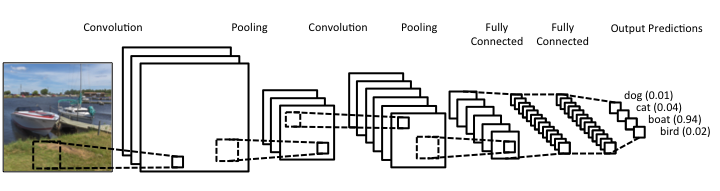
\includegraphics[width=1\textwidth]{Figures/cnn.png}
  \caption{ Overview over a sample Convolution Neural Network, From left to right the input image is processed by convolutional layers, pooling layers and last by fully connected layers, which output a prediction}
\end{figure}
Convolutional neural networks or CNNs are particularly important for deep reinforcement learning on video games. CNN's are what make it possible to directly use the rendering output of the game as the environment's observations. They are very similar to regular neural networks in that they still have interconnected layers with learned weights, have a loss function on the last fully connected layer, and still express a single differentiable function from input to output. The biggest difference to a regular neural network is that a CNN explicitly assumes that all inputs are images in the form of raw pixels, and has specific architecture to deal with them.

The original architecture for CNNs is the LeNet architecture \citep{leCun}, proposed in 1998. 
While there have been developed many new architectures since, like AlexNet\citep{alexnet}, GoogleNet \citep{googlenet}, or ResNet \citep{DBLP:journals/corr/HeZRS15}, which improve greatly on it's effectiveness, most of these architecture still make use of the same or at least similar building blocks to create the neural network.   
These components are

\begin{enumerate}
\item Convolution
\item Activation Function
\item Pooling
\item Fully Connected Layers
\end{enumerate}

During the convolution step a series of filters is applied to the image. In addition to the neuron weights, the convolution filter values are learned by the CNN as well. The size, number, and stride of these filters is specified before training though and can be treated as hyperparameters. After training each of these filters represents one feature, that has been learned by the network.
The activation function, most notably a linear Rectifier(RelU), is applied after each convolution step. This is done in order to bring non-linearity into an otherwise linear system. This is important, as the real world can rarely be described in completely linear terms.

Pooling Layers drastically reduce the size of the convolved images by grouping nearby pixels together and taking for example their maximum, minimum or average value as the pixel value for the resulting image. This increases training speed, but more importantly leads to translation invariance in regards to the input.

Components 1. till 3. can be chained together multiple times before flattening their output into a single feature vector and then following up with one or multiple fully connected layers. These fully connected layers can either be normal neural network layers or more specialized layers like for example RNN layers or the LSTM layers described in the following section.


\subsection{Long Short-Term Memory Networks}
\label{sec:lstm}
LSTM units \citep{lstm,DBLP:journals/neco/GersSC00} are a form of recurrent neural network layer, that is especially adept at discerning temporal dependencies between subsequent inputs. Since temporal dependencies tend to be quite important when interacting with an environment like in reinforcement learning, LSTM layers can be an excellent choice for function approximation. 

Nevertheless, they require the training samples generated by the reinforcement learning algorithms to be processed in the correct temporal order. As the A3C algorithm is an inherently asynchronous algorithm, that can not guarantee the order in which the samples are added to the training queue, LSTMs were not used in this project. While the ACKTR and A2C algorithms are synchronous, and the A2C algorithm even comes with an optional LSTM policy, this policy was not used and instead all of the algorithms use the same basic CNN policy. 

\section{Asynchronous Advantage Actor-Critic (A3C)}
\label{sec:a3ctheory}
\begin{figure}[htb]
  \centering
      \includegraphics[width=1\textwidth]{Figures/A3C_Overview.pdf}
  \caption{ Overview of the general A3C Architecture. Multiple workers interact with their own environments in parallel and trade their learned information with one global network }
  \label{fig:a3cover}
\end{figure}

The A3C algorithm is a somewhat recent reinforcement learning algorithm released by Google's DeepMind team \citep{DBLP:journals/corr/a3c}. It became very popular very fast, as it made Deep Q Networks, which were incredibly popular before, practically obsolete. It performs not only better and more robustly, but from own experience it is also easier to implement.

As the name implies it is an Actor-Critic reinforcement learning method as described in section \ref{sec:accritic}. But, instead of one actor-critic pair working on one environment, A3C makes use of multiple Workers, that each have their own Neural Network parameters and interact with their own environment as illustrated by Figure \ref{fig:a3cover}. The samples generated by these workers are then played back asynchronously into one global network. This is preferred over the single environment approach, because, in addition to the performance benefit of parallel processing, all of these Workers are independent from each other resulting in much more diverse samples.

This global network has one input, the current state $s$ and two distinct outputs: a softmax activated probability distribution $P$ over all actions $a$ acting as the policy 
$$\pi_\theta(s)$$
and an estimate of the value function for the input state.

The "Advantage" part of the algorithm's name comes from the use of the advantage value $A$ during the policy gradient step instead of the discounted reward $R$. The advantage estimate helps the agent to not only establish how good a given action is, but also how much better it turned out than expected.
The advantage value can be calculated using:
$$A = Q(s, a) - v(s)$$ 
As A3C does not approximate $Q(s, a)$ directly, it is replaced by the discounted reward $r$.
This reward $r$ is calculated as an n-step discounted return, utilizing a forward view. This means, that updates to the network parameters can not be applied immediately and instead have to be processed in batches in order to calculate this n-step return. While this introduces policy lag, this was found to be easier than using a backward view with eligibility traces in some cases.
For exploration purposes entropy should be added to policy $p$ as well, as otherwise a convergence to local minimums is likely. The loss function to be optimised therefore has 3 components and is defined as: 
$$L_{total} = L_{\pi} + L_{v} + L_{entropy}$$
The policy loss $L_{\pi}$ describes the total reward that an agent can achieve averaged over all starting states, and is calculated as
$$L_\pi = E[A(s, a) * log \pi(s, a)]$$
This is the expected advantage value over the probability distribution of policy $\pi$. For batch processing this policy loss is additionally averaged over all samples.

The value loss $L_v$ utilizes the fact, that the true value function is estimated in accordance with the Bellman Equation. 
$$V(s_0) = r_0 + \gamma r_1 + \gamma^2 r_2 + ... + \gamma^n V(s_n)$$
With an n-step return the loss is the difference, between the current estimation of rewards of a state, and the estimation after n steps.
$$L_v = r_0 + \gamma r_1 + \gamma^2 r_2 + ... + \gamma^n V(s_n) - V(s_0)$$
Again, this loss is averaged over all samples in a batch.

Maximizing the entropy pushes the policy away from a fully deterministic policy. The entropy for a single sample can be defined as
$$H(\pi(s)) = \sum\limits_{a} \pi(s)_a \cdot log \pi(s)_a$$
with $\pi(s)_a$ being the probability of taking action $a$ while in state $s$.
To get the  full $L_{entropy}$ one again averages over all samples and then negates the result, as the loss function is minimized and the entropy has to be maximized.
$$L_{entropy} = \sum\limits{i=1}^{k H(\pi(s_i))}$$

The optimization of this loss function could be done by Stochastic Gradient Descent as shown in section \ref{sec:sgd}, but RMSPROP \citep{rmsprop} has been shown to be the most robust \citep{DBLP:journals/corr/a3c}.

One slightly different version of the A3C algorithm is the A2C algorithm that was released in conjunction with the ACKTR algorithm by OpenAI\citep{openaiblog-a2c}. A2C is used for testing in this project as well and is closely related to the A3C algorithm. Essentially it is simply a synchronized variant of the same algorithm, hence the name "Advantage Actor-Critic". Tests done by the OpenAI team show, that the asynchronicity of A3C does not result in tangible performance benefits\citep{openaiblog-a2c}.

\section{Actor-Critic Kronecker-Factored Trust Region (ACKTR)}
\label{sec:acktrtheory}
ACKTR, proposed by a group of researchers from both University of Toronto and New York University in late 2017\citep{DBLP:journals/corr/abs-1708-05144} is an even more advanced and state of the art algorithm than A3C. The authors posit, that sample efficiency is the primary metric of concern for reinforcement learning algorithms. In both simulated and even more so real world environments getting training samples and stepping through the environment is much slower than the actual processing of the algorithm. For that reason the authors propose an algorithm that manages to learn complex problems much faster than other algorithms with being around 25\% slower to compute but being much more sample efficient.

Most reinforcement learning algorithms use relatively simplistic optimization techniques like stochastic gradient descent, that are rather inefficient. ACKTR however aims to utilize more sophisticated optimization strategies, while employing and combining ideas from multiple different reinforcement learning algorithms.

Similar to A3C and A2C algorithms for example ACKTR is an actor-critic algorithm that uses multiple environment workers to reduce training time and increase sample diversity. Yet, the optimization is an extension of the optimization of the natural policy gradient algorithm.

The problem with the natural policy gradient is, that the natural gradient can not be directly computed and has to be estimated. Trust Region Policy Optimization(TRPO) \citep{DBLP:journals/corr/SchulmanLMJA15} is one of the algorithms that does that, but TRPO is sample inefficient and does not lend itself to be used with large models.

The key idea of the ACKTR algorithm is to calculate this gradient by using Kronecker-factored approximated curvature(K-FAC)\citep{DBLP:journals/corr/MartensG15}.
Gradient updates using K-FAC only take marginally longer to compute than an SGD update, but utilizing a natural gradient makes this algorithm much more sample efficient.

\section{Reinforcement Learning in StarCraft}
The primary paper building the basis for this thesis is StarCraft II: A New Challenge for Reinforcement Learning \citep{DBLP:journals/corr/dmsc2}. This paper introduces the PySC2 framework and offers evaluations for basic scenarios that were gained using some of DeepMinds own Neural Networks. These scenarios are largely abstract and very simple however, and do not reflect the actual competitive game of StarCraft II. This thesis aims to improve that aspect.

DeepMind implemented the A3c algorithm either using the AtariNet, which DeepMind used to successfully learn a multitude of Atari Games or FullyConvNet, a fully convolutional Neural Net with no fully connected layers but optionally with LSTM layers. 

As both PySC2 and the StarCraft II Machine Learning API have been released there are only very few scientific articles that make use of them. There are however a considerable amount of papers on StarCraft II's predecessor, StarCraft: Broodwar. It's API, while not officially endorsed by Blizzard has been around for many years and has gathered a sizeable community.

While papers on StarCraft: Broodwar are not fully applicable to StarCraft II there are considerable similarities in the gameplay of these two games, making these papers at least somewhat related. 
Among these papers is \citep{broodwarRL}, which is the namesake of this thesis and the paper the idea for this thesis comes from. This paper explores the StarCraft:Broodwar API at the example of one small combat scenario utilizing Q-Learning and SARSA algorithms and evaluates their suitable in that context. It was able to achieve decent success in that specific scenario through the usage of highly abstracted actions, and a very limited action and observation space. The scenario in question is further discussed in section \ref{sec:failed}.

A very similar topic, unit micro-management, is discussed in the paper \citep{scai:unitmicro}, and a more general view on combat in Real-Time-Strategy(RTS) games can be found in \citep{scai:gamecombat}. There are also a considerable amount of papers on other aspects of StarCraft reinforcement learning, that do not directly relate to combat scenarios. \citep{scai:bo} for example concerns itself with the planning of build orders for optimal economic growth.

\section{Non RL StarCraft AI(Bots)}
Before reinforcement learning became relevant for StarCraft AI there was already a sizeable community around writing regular AI bots. While they are only peripherally related, they can give insights to interesting scenarios and problems for StarCraft Bots, while also being a useful benchmark. \\Although not available in the form of scientific articles, the most popular hard-coded bots are automaton 2000 and Ursadak. Both of these Bots leverage tens of thousands of actions per minute as their main advantage. Automaton 2000 for example executes approximately 100 actions per minute(APM) per single unit that it controls. No human, and likely also no reinforcement algorithm can come close to that number, especially with larger unit groups. Sometimes they even employ borderline cheating for even more impressive results. Figure \ref{fig:aut} shows an example of that. 

\begin{figure}[htb]
  \centering
      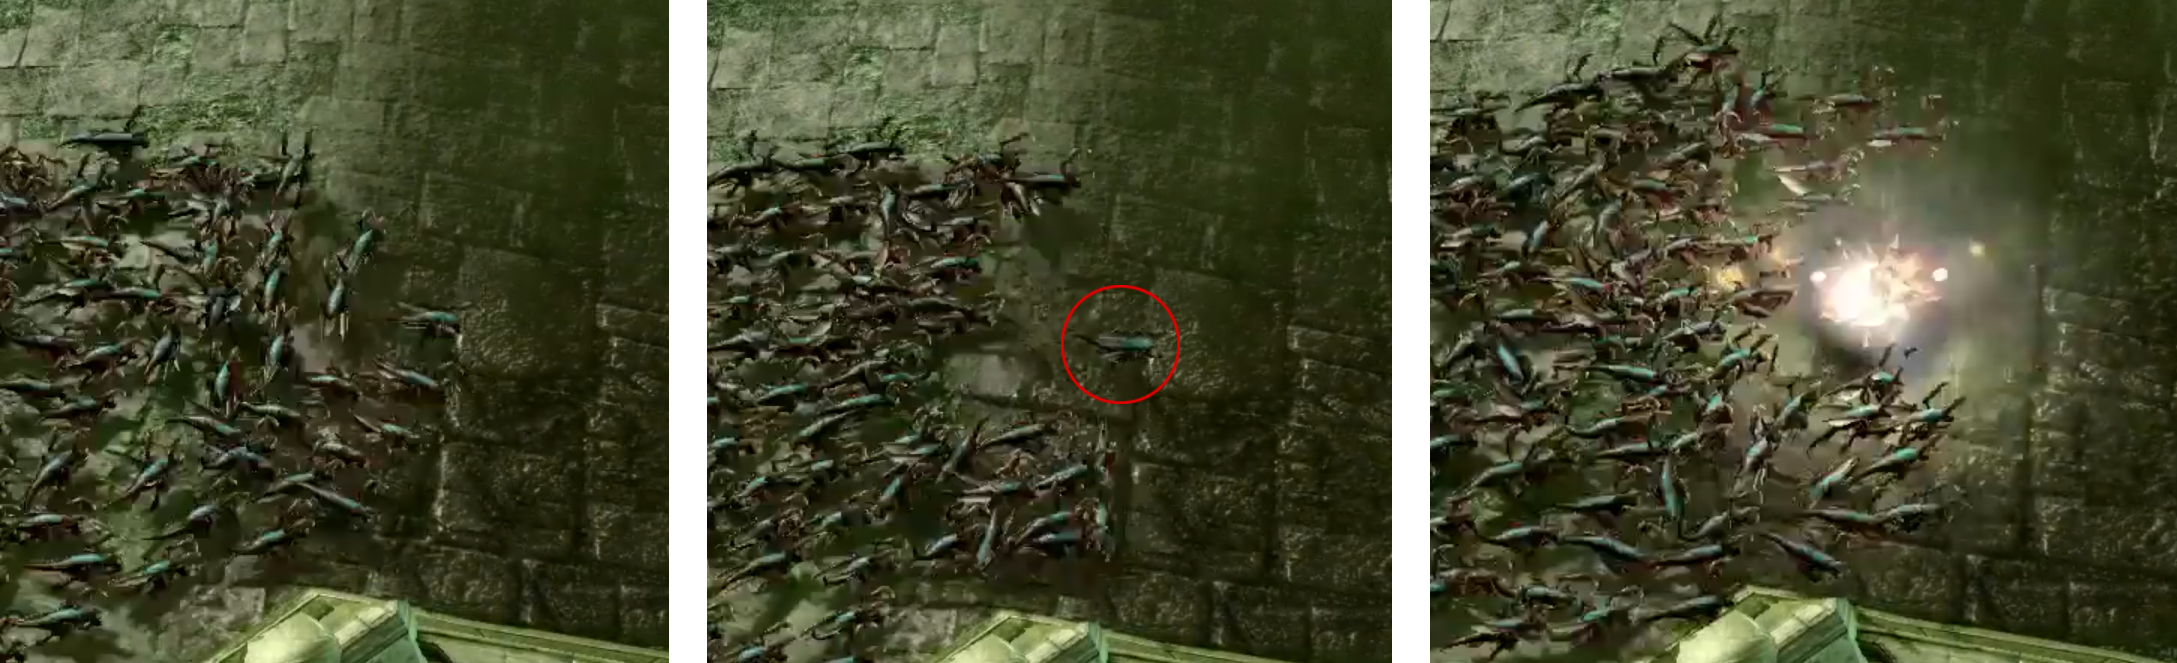
\includegraphics[width=1\textwidth]{Figures/aut2000.png}
  \caption{ Example of advanced techniques used by microbot AUtomaton 2000. With knowledge of which unit an area of effect attack is going to land it can split its army in order to minimize the damage incurred.}
 \label{fig:aut}
\end{figure}

Automaton manages to figure out which of its units is targeted next by enemy fire, information that should not be available and at least is not available to human players. With its high APM it can use this information for pulling away units nearby the targeted unit in the event of an area of effect attack, thus preventing almost all damage of the attack. In the video this Figure is taken from, 100 Zerglings are pitted against 20 Tanks, tanks being AoE(Arrea of Effect) attacking units specifically designed for defeating large groups of Zerglings. In this test and without the microbot, all Zerglings are defeated without destroying more than 2 tanks. With microbot's active micromanagement however, all Tanks are defeated, after which about a dozen of Zerglings are still left alive. 

This shows how potent this combination of high APM and usually not available or hard to obtain information is. In contrast to Automaton 2000, Ursadak is not only a microbot, that concerns itself solely with the micromanagement of units, and instead is a fully featured bot, that is able to play the complete game of StarCraft II as the terran race. While there are many more bots and especially microbots for StarCraft II, these are 2 of the more popular ones, having been featured on prominent StarCraft II tournaments for showcasings. There even are full AI only tournaments where Bots battle each other either in specialized scenarios, or the actual games of StarCraft/StarCraft II \citep{scai:comps}.




 
% Chapter 1

\chapter{Starcraft II} % Main chapter title

\label{chap_sc2} % For referencing the chapter elsewhere, use \ref{Chapter1} 

%----------------------------------------------------------------------------------------
\section{Gameplay Basics}
Both Starcraft II and its Predecessor are Real Time Strategy(RTS) games set in the future. They are 2 of the most successful video games of their genre, with millions of players and active competitive scenes that award millions in tournament prizes each year. 

In StarCraft (II) the players take on the roles of the commanders of three different factions: Terrans, Zerg and Protoss.
While there is a single player campaign, the by far most played game mode is the competitive multi player 1 vs 1 ladder.
In this game mode the player starts with his races' main building and a group of workers.
His goal is to mine the 2 available resources Minerals and Gas with his workers and use these resources to build a base, by constructing different types of buildings and create an army using the unique unit types that are available to each race. While building and expanding his base and resource income the players use their units to attack their opponents' base or defend from their opponents' attacks. The game is over, when one player either gives up or has no more buildings on the map. This game mode is played on a number of different maps that offer distinct strategic possibilities through various base layouts, attack paths etc.

As a strategy game there are of course many different strategic choices to make.
These include when and how to build and expand your base, what unit composition to build your army with, when and where to attack and so on.
Much more than strategy, Starcraft II emphasizes the Real-Time aspect of RTS though. The main problem a Starcraft II player faces is how to to manage all the individual aspects of the game, like base building, managing the economy, scouting, micromanaging your army etc. simultaneously and as fast as possible. Even professional players, players that can often reach 300 Actions per Minute(APM) or more, can not multi-task efficiently enough to manage all these tasks perfectly. Such high APMs are achieved through the heavy use of hotkeys for unit and building groups, unit abilities and commands, and more.
In general, the game is controlled using Mouse and Keyboard, where the Keyboard is used mainly for around 30 different hotkeys and the mouse is used to move the screen around the map, select units or buildings and confirm orders needing a target mouse position.

In addition to multitasking another important challenge in Starcraft II is limited information. Due to a "Fog of War" that spans the entire map each player has only visibility in a small radius around each building and unit he owns. That means the players need to constantly scout the map and their opponent to get the information they need to make the correct Strategic choices.
There is also an inbuilt AI available in different difficulties that players can play against. This AI is hardcoded using traditional programming however and does not make use of machine learning. It is also very weak and should, even in the hardest difficulties that resort to cheating, prove almost no challenge to a decent Starcraft II player.

\begin{figure}[htb]
  \centering
      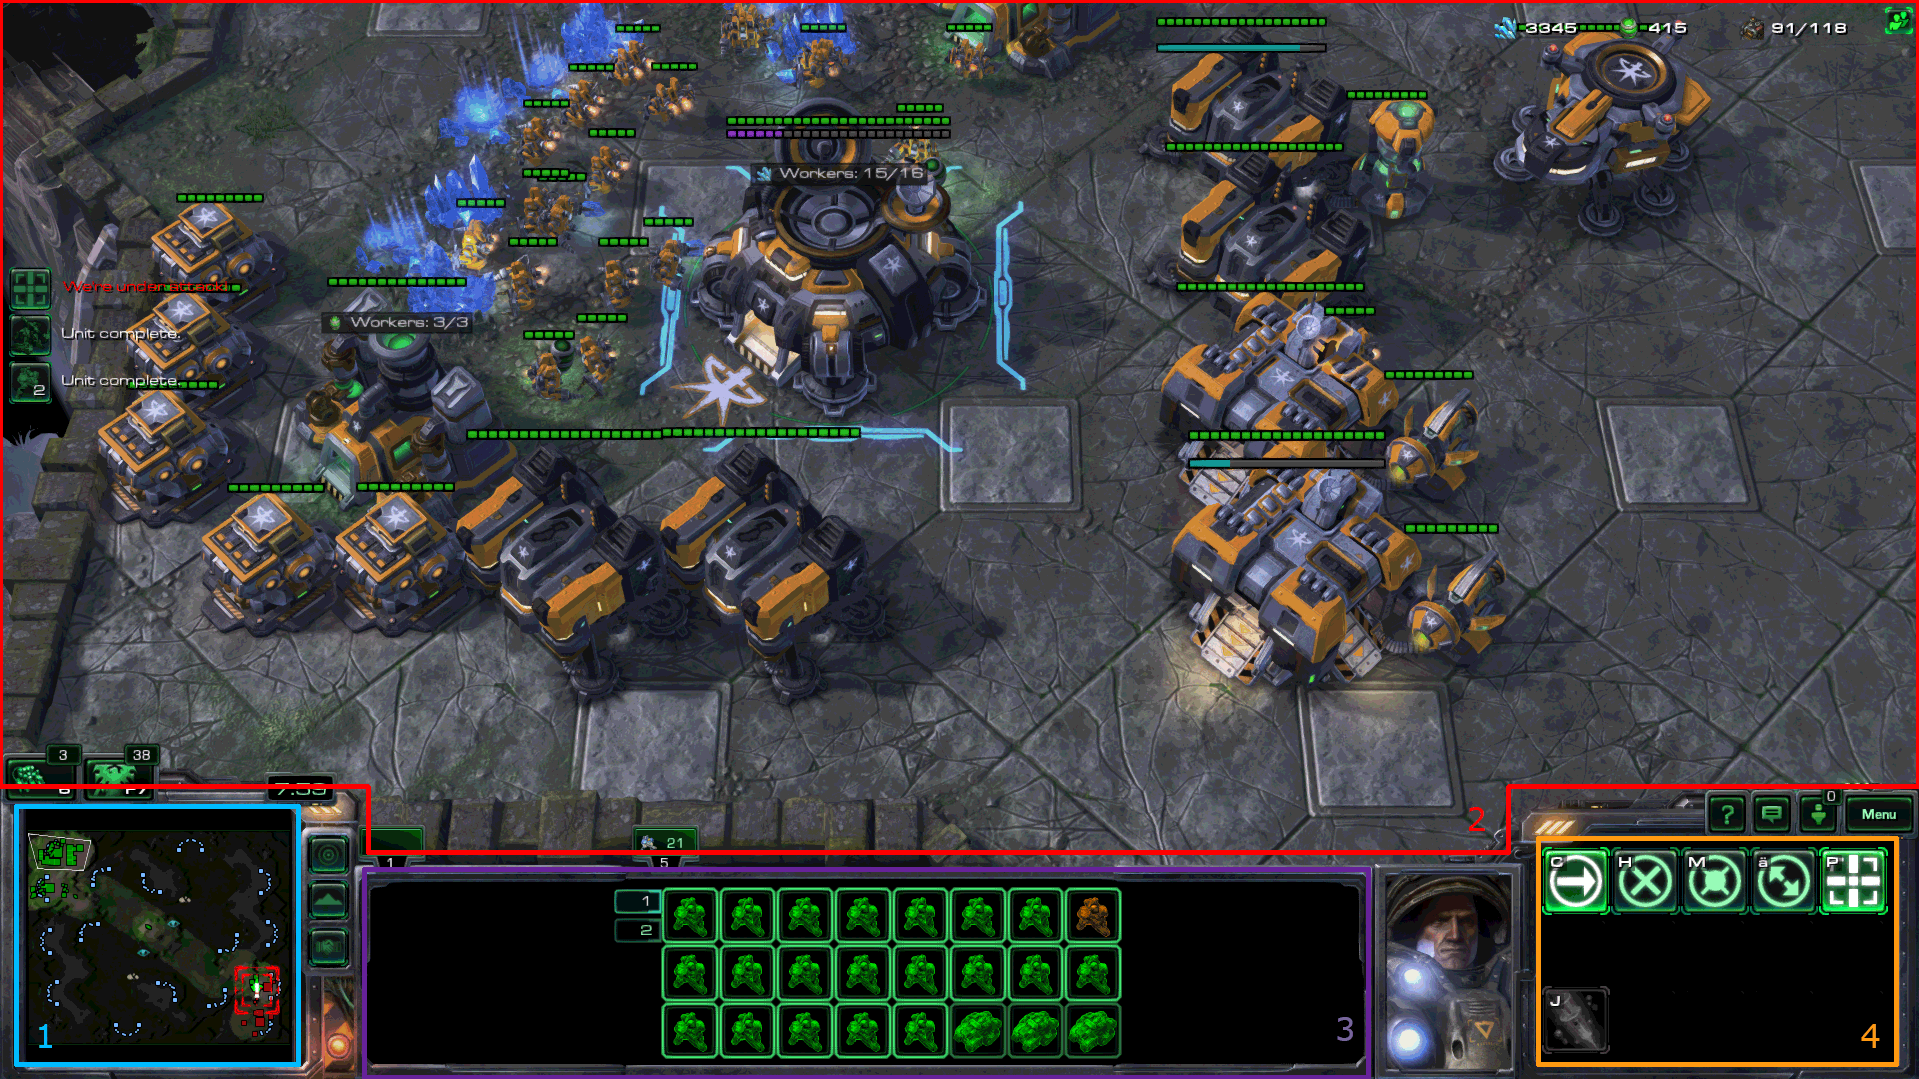
\includegraphics[width=1\textwidth]{Figures/gameview_bordered.png}
  \caption{The StarCraft II Ingame User Interface: 1 - Minimap view of the entire Map with white trapezoid showing current screen section, 2 - Main Game View, 3 - overview of currently selected unit(s), 4 - Command Palette of first unit type in selected units}
  \label{fig:gameview}
\end{figure}

Figure \ref{fig:gameview} show the default User Interface for a Terran player. The red bordered part of the screen is the main game view, that shows the actual game. Green bars over the units and denote their current hitpoints and change color depending on how much damage a unit has taken. Bordered in Teal is the minimap, which shows a minified view of the entire map with the white trapezoid being the section currently shown in the main game view. Friendly Units on the minimap are depicted in green, neutral units in yellow and enemy units in red. The purple section contains information about the currently selected units. Each square represents one unit and their color mirrors the color of their healthbar. The orange bordered section contains the command palette of the selected units or buildings, showing all actions that can be executed. Temporarily unavailable actions are greyed out. If multiple types of units are selected like in this screenshot, only the command palette for the first type of units is shown. That means that only their special abilities can be executed by a simple click or hotkey, using abilities of other unit types requires additional switching of the active unit type.


\section{Starcraft II as a Reinforcement Learning Environment}
The StarCraft games are well known as being very difficult to play both mechanically, meaning multitasking and just the general control of your mouse and keyboard, and strategically. The games have an incredibly high skill ceiling with even professional StarCraft players still making mistakes almost every game even after decades of competitive play and daily practise. The mechanical aspect of the game is where a computer should have a big advantage over human players as humans are physically limited in their APM. Strategy is something that one can expect an algorithm to struggle with much more, because it is a very creative and abstract aspect of the game. Both the mechanics and the strategy contribute to the high degree of  depth and complexity in the game. 

One tool that makes StarCraft II especially suited as a reinforcement learning environment is it's very powerful Map Editor. 
The StarCraft II Map Editor has played a big role in the success of Blizzard's Starcraft and also Warcraft video game franchises of Blizzard. It allows not only to create new maps for standard game modes, but gives so much freedom and access to game data and scripts, that it is very easy to create entirely new game modes that are entirely different. So much so, that sometimes the base game is barely recognizable anymore, because the game might not even be an RTS type game mode anymore. The most popular Genres of custom modes, also called "Fun Maps" or "UMS(Use Map Settings)"
 include Role Playing Games(RPGs), Co-Op shooters, Tower Defense, Survival, and many more.
 
Taking into account custom maps and game modes makes the number of possible scenarios that can be explored in StarCraft II using reinforcement learning almost infinite. Both this and the complexity of the game itself make for an, in my opinion, very interesting reinforcement learning environment. And, as demonstrated by the failure of the Deepmind Team to beat even the worst inbuilt AI using reinforcement learning \citep{DBLP:journals/corr/dmsc2}, it is an environment that will likely continue to present interesting challenges for AI Research in the foreseeable future.
 
% Chapter 1

\chapter{Starcraft II Machine Learning API} % Main chapter title

\label{chap_api} % For referencing the chapter elsewhere, use \ref{Chapter1} 


%----------------------------------------------------------------------------------------

\section{Environment}
The PySC2 Environment used in this thesis is a python layer on top of the Starcraft II C++ API.
Both of these APIs are relatively new and are still constantly being developed, with new features and actions being added as they evolve. Also, at least the PySC2 API, is still getting big overall changes, that sometimes can even break existing programs relying on an older interface.
PySC2 has been developed specifically for the exploration of reinforcement learning algorithms by a Team of DeepMind developers in collaboration with Blizzard.

\begin{figure}[htb]
  \centering
      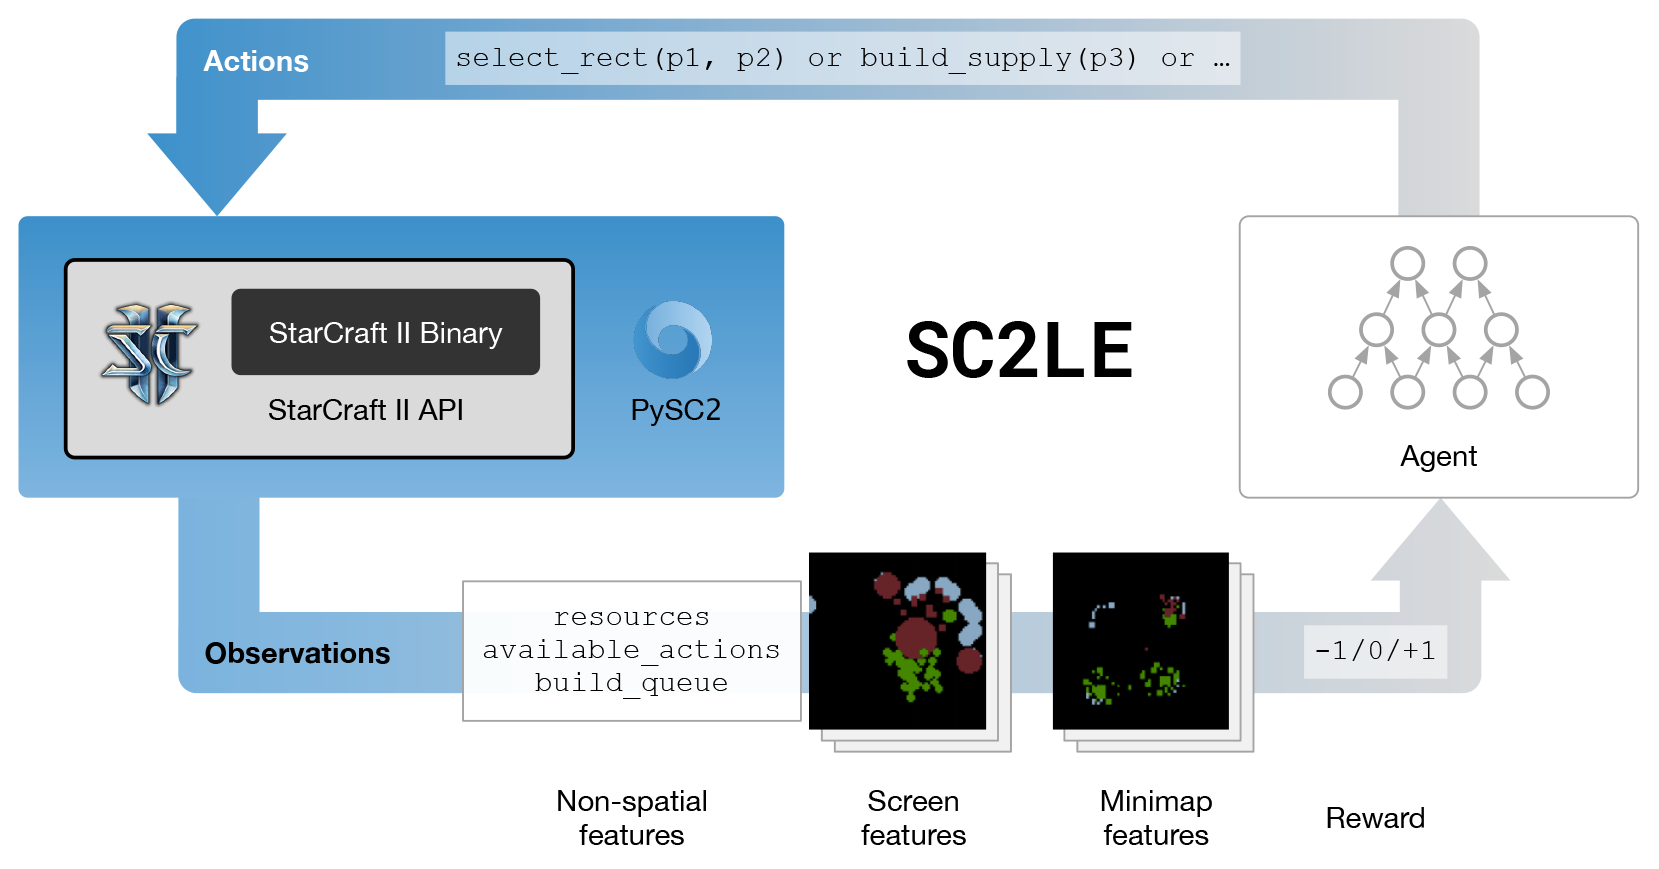
\includegraphics[width=1\textwidth]{Figures/sc2le/sc2le_overview.png}
  \caption{An overview over how an agent interacts with the PySC2 environment. The environment delivers observations in the form of spatial(screen, minimap) information and discrete information. The agent then takes an action in the environment and the cycle continues\citep{DBLP:journals/corr/dmsc2} }
  \label{fig:pysc2_overview}
\end{figure}

Figure \ref{fig:pysc2_overview} shows how the communication between PySC2 and an agent works. PySC2 functions as a wrapper to the StarCraft II machine learning API, which in turn is a wrapper on top of the actual StarCraft II game engine. For each iterative step of an episode the agent can acquire observations for the current state from PySC2 in the form of different types of features. The agent then chooses PySC2 actions on the basis of these observations, which are then executed by PySC2 leading to a new state and thus new observations. This cycle continues until an episode is over.    



\begin{figure}[htb]
  \centering
      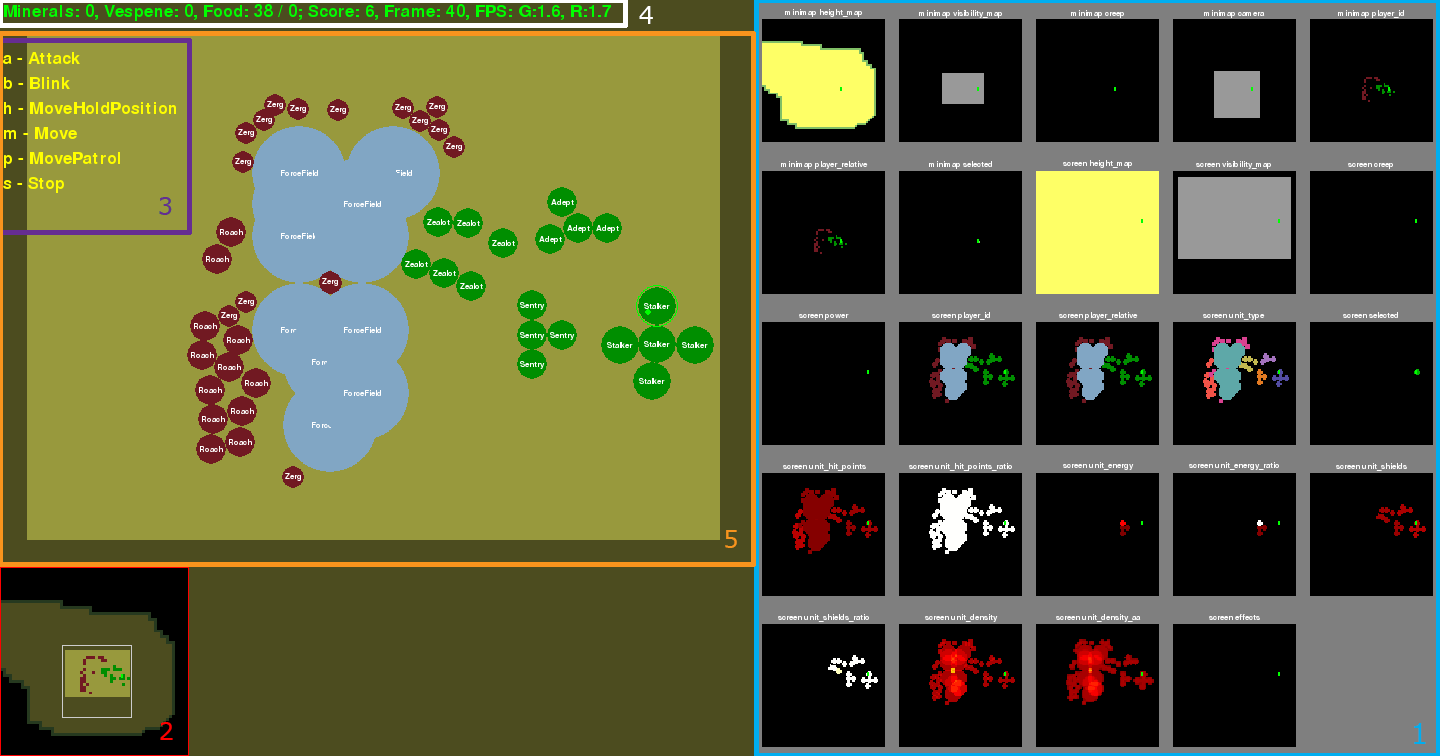
\includegraphics[width=1\textwidth]{Figures/pysc2_borders.png}
  \caption{PySC2 rendered debugging view: 1 - current state of feature layers, 2 - Minimap rendering, 3 - List of available commands, 4 - List of some of the discrete values, 5 - Approximate Game State Render}
  \label{fig:pysc2_render}
\end{figure}
Figure \ref{fig:pysc2_render} shows the debugging view that is provided by the pysc2 framework. This view is particularly important for users of the headless linux client, as the headless client does not offer rendering on it's own as opposed to the Windows and Mac clients.

The right half of this view contains image representations of all feature layers available within PySC2. Section \ref{sec:pysc2_features} discusses those features in greater detail. Altough some of the feature layers in this debug view seem to be multi-colored, this is done only for easier human interpretation. The actual feature layers are all single channel images. Bordered in orange and red are pysc2's depictions of a simplified game view and minimap respectively. On the left side in purple is a list of hotkey - action pairs, that are currently available to player 1. These actions are not stictly StarCraft II actions but specifically PySC2 actions. The top row of information bordered in white is a list of discrete values that PySC2 offers.


\newpage
\subsection{Framework/Engine Parameters}
\label{sec:engparam}
In addition to the specifics of the scenarios created in the Map Editor there are a few parameters for the PySC2 Framework and StarCraft II client, that shape the overall reinforcement learning environment.
Some of the most important are listed here. 

\begin{itemize}  
\item map name - The name of the Map that will be run.
\item screen resolution and minimap resolution - The resolution at which the screen and minimap input layers are rendered by the PySC2 framework.
\item render - A Boolean whether to show a debug view (cf. Figure \ref{fig:pysc2_render}), showing all feature layers and a game view.
\item step multiplier - How many game steps should be taken for every agent step. 
\item score index - Which type of scoring to use. -1 denotes a simple Win/Loss score on a per episode basis. Values >= 0 denote scoring categories within the game with 0 being the cummulative Score.
\item difficulty - the level of AI the agent will play against. 
\item save\_replay - whether StarCraft II should save a .sc2replay file, that can be played back later (can only save roughly 2 million game steps)
\end{itemize}

The screen and minimap resolutions and the step multiplier are particularly important for the performance of reinforcement learning algorithms.
The step multiplier gives control over how often the agent is allowed to act. The game logic itself is calculated at 24 frames per second, meaning that an agent can take a maximum of 24 actions per second. Yet, for most applications this is much too fine-grained and results in too long episodes. The default value of eight game steps per agent has the agent take three actions per second. This is equivalent to a decent to good human player. Of course, if the goal is to beat professional players in complex scenarios increasing this value is unavoidable.

The rendering of the input layers is a very CPU intensive task and a major contributor to the slow performance of the PySC2 environment, which is why setting appropriate screen and minimap resolutions is important. Ideally they should be set as low as possible, while still accurately portraying the game world. The default value of 84 pixels for the screen resolution was used in this project.



\subsection{Features}
\label{sec:pysc2_features}
There are two ways in which PySC2 deals with observations/features. Most of the important features are organized in layers,
and layers in turn are organized in minimap layers and screen layers. Each layer is a very coarsely rendered image map of one specific type of information. The screen layers contain information for the currently active screen of the player, and the minimap layers contain information for the entire map. Using similar resolutions for both map types, which is the default, therefore results in very inaccurate minimap layers that can often miss information. This represents the actual game when it is played by a human though, as the minimap only takes up a very small area on the screen and is only supposed to contain very rough and general information.

As stated in a previous section, the number of layers is still increasing, but at the time of writing there are layers for most of the important types of low level information in the game already available. These include unit type, unit health/shields, unit player affiliation, player visibility, terrain elevation and more.
The second group of features are a set of discrete values, that are not related to screen or minimap coordinates and therefore dont lend themselves well for usage in an image map. Available as discrete values are for example the current resources(minerals, gas, and food) of the player, the current score and saved unit group hotkeys.
The feature layers used specifically in the project for this thesis are

\begin{itemize}
\item player\_relative - Used by all scenarios, it contains pixels with one of five values: 0(No unit), 1(Friendly unit), 2(allied Unit), 3(neutral unit), 4(Enemy unit)
\item creep - values of 0 or 1 depending on whether the terrain is coated with creep or not
\item selected - Values of 0 or 1 depending on whether a unit on the pixel is currently selected by player 1
\item height\_map - values of 0 to ~180 according to terrain elevation, 0 being flat ground
\item unit\_type - values of 0(No Unit) to ~400, representing the id specifying the type of unit on a pixel
\item unit\_hit\_points and unit\_hit\_points\_ratio - How much current health a unit on a pixel has left. The layer unit\_hit\_points contains absolute hit point values, whereas unit\_hit\_points\_ratio contains percentage values normalized to a 0 to 255 range
\item unit\_energy and unit\_energy\_ratio - How much ability energy a unit on a pixel has currently left. As with the hit points layers unit\_energy contains absolute values and unit\_energy\_ratio contains percentages
\end{itemize}
As can be seen, most of these layers have different value ranges and are not normalized to a desired 0 to 255 spectrum that would lend itself well for CNN's. While for some layers like the "creep" and "selected" layers the normalization is trivial, other layers like unit\_type can not easily be normalized, as they contain more than 256 values and floating point values should be avoided.


\subsection{Actions}
Actions in the PySC2 environment work somewhat differently than could be expected in a reinforcement learning environment. Instead of simply having an array of actions, all actions in PySC2 require a number of additional arguments. Most notably many actions need screen coordinates, or information on whether the actions is supposed to be executed directly, or put into an action queue in order to be executed later. 

The actions available in PySC2 are very low level and close to the actions that a human would take, with some simplifications. For example, most actions executed by humans need both a keyboard shortcut(or click on ability symbol) and a mouse click on screen, while PySC2 combines these actions into one. This helps considerably with the limited APM a reinforcement learning algorithm can employ and makes a great deal of sense, as each of these components on their own do not make a successful action.

\begin{figure}[htb]
  \centering
      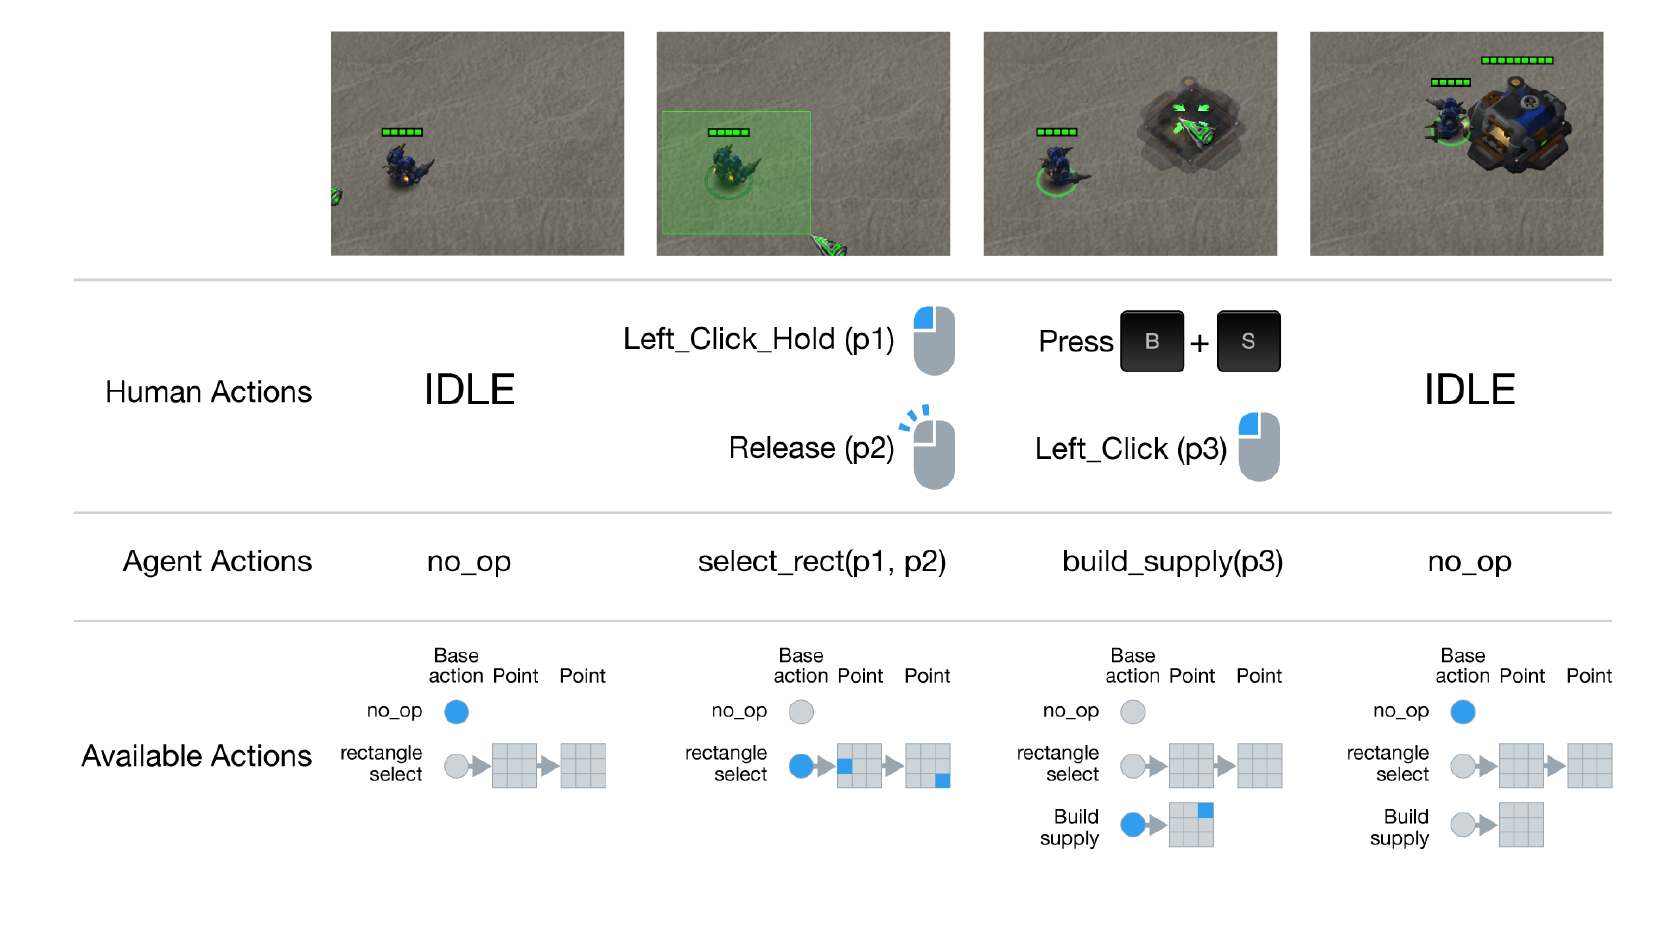
\includegraphics[width=1\textwidth]{Figures/sc2le/sc2le_actions.png}
  \caption{From left to right: a progression of actions and comparison between human actions and the corresponding pysc2 actions \citep{DBLP:journals/corr/dmsc2} }
  \label{fig:pysc2_actions}
\end{figure}
Figure \ref{fig:pysc2_actions} illustrates a sequence of actions a unit could take and how they relate to PySC2 actions. The sequence starts with an idle state, after which the human selects the unit using a rectangle selection and then orders it to build a supply depot. For the actual order to build the supply one can see that even 3 human actions have been combined into a single PySC2 action.


A list of all available actions and their respective arguments can be viewed by executing
\begin{lstlisting}[language=Python]
python -m pysc2.bin.valid_actions
\end{lstlisting}
after installing pysc2. Not all of these actions are available at all times however, as many of these actions depend on having a specific unit or building currently selected.
The actions utilized in the scenarios for this thesis are:
\begin{itemize}
\item No\_op - Have the agent execute no action at all, needs no additional arguments. This is useful in case the current state is preferable over all states that can be achieved by taking an actual action.  
\item Select\_Army - Selects all units belonging to the player on the entire map
\item Move\_Screen - Orders all selected units to move to the specified screen coordinate, without attacking enemy units until the location is reached
\item Attack\_Screen - Similar to Move\_Screen, but ordered units will attack all enemy units they encounter until reaching their destination
\newpage
\item Select\_Point - Selects the unit present at the specified screen coordinate, deselecting all previously selected units. If a friendly unit is selected, it can also be added to the current selection of units instead through the use of the 'shift' modifier in game, or an additional argument in PySc2. In contrast to the real game, enemy units can not be selected at all in PySC2 however. Selecting the background, and in PySC2's case selecting enemy units results in deselecting everything.
\item Effect\_ForceField\_Screen - Orders one of the selected sentry units with enough energy left, to spawn a forcefield at the specified screen coordinate. Will fail if no sentry unit has enough energy. If no sentries are in range of the specified point, one of them will automatically move closer and spawn a forcefield once in range.
\item Effect\_Blink\_Screen - Orders all selected Stalker units to Blink to the specified screen location. Similar to the Force Field ability of the sentry all Stalkers move close enough to the point in order to execute the Blink ability. 
\item Guardian\_Shield\_Quick - Orders one of the selected sentries with enough energy to erect a shield around itself and nearby friendly units by executing the Guardian Shield ability
\end{itemize}

One of the most important actions for human players, \lstinline{select_rect} has been intentionally left out in this project. This is due to the fact, that it is the only available action that not only uses one set of coordinates as parameters, but needs two, one for the upper left and one for the lower right point of the rectangle. This necessitates a different neural network model and increases complexity by a considerable amount(At a resolution of 84 the \lstinline{select_rect} action alone would make for an action space of $84^4$ ). This rectangle selection is commonly used in order to select groups of units. The Rl algorithm instead relies solely on the \lstinline{select_point} method.



\section{Classic Starcraft vs Starcraft II}
In addition to the Starcraft II API there is also a machine learning API for the classic Starcraft: Broodwar.
As both of these games are very similar in their gameplay elements this section illustrates some of the differences of their respective APIs and conclude with why the Starcraft II API was chosen for this thesis.

In contrast to the Starcraft II API input layers, the Starcraft: Broodwar API exposes the features of the environment in an object oriented way. This means, that all players, units, etc. are available as nested objects with discrete values. If, for example, one wants to get all the units of a player one would only have to call getUnits() on the player object and get a list of unit objects with discrete values for position, health, etc.. So while CNNs are almost required for writing bots using the Starcraft II API they are not very useful in the Starcraft: Broodwar API. Not only the features are seperated and bound to these objects though, the actions have to be called on the objects themselves aswell. Hence, ordering a unit to attack would involve simply calling the attack() method on the unit object. 

While this structure of features and actions might seem simpler, it is very unorthodox when considering standard reinforcement learning algorithms and techniques. The Starcraft: Broodwar seems to have been written as a general API for developing Bots with many different technologies and not specifically with reinforcement learning in mind. 

The biggest advantage, that the Starcraft: Broodwar API has to offer for the use in my thesis is that it has been in developement for a much longer time of approximately 3 Years. Accordingly, a community has formed around this API with numerous academic papers being written and examples and tutorials for bots readily available. There are even regular tournaments for StarCraft: Broodwar bots in which teams, mostly universities, let their bots battle against each other. The most notable example is the SSCAIT, which is both a tournament and a ladder \citep{sscait}.

This is opposed to the StarCraft II API, which is very new and therefore has not yet developed such a community.
Also, the StarCraft: Broodwar API offers a full documentation whereas with the StarCraft II a lot of time has to be spend directly looking into the code of the API.

These advantages where however not enough to convince me to use the StarCraft: Broodwar API.
In the end the StarCraft II API was chosen, and specifically PySC2, because it is state of the art, actively being developed, and because it is specifically designed for the use in with reinforcement learning algorithms.


 
% Chapter 1

\chapter{Project} % Main chapter title

\label{chap_prac} % For referencing the chapter elsewhere, use \ref{Chapter1}

%----------------------------------------------------------------------------------------

This chapter will discuss the accompanying project to this thesis in it's entirety. First, section \ref{sec:idea} will describe again the general idea of this project, and section \ref{sec:fworks} will list some of the external tools that were used to implement this project. Afterwards section \ref{sec:mapedit} will cover how the test scenarios for this project were build and some of the tools of the StarCraft II Map editor that are available for this task.
Then, section \ref{sec:scenarios} will go into detail about the specific scenarios that were tested, and the strategies that were expected to be learned. Next, the overall architecture of the project and some of the general modules are depicted in section \ref{sec:rlfwork}. The following sections \ref{sec:ac3impl} and \ref{sec:baselinesproj} will detail how the A3c algorithm and the Open AI Baselines algorithms (ACKTR, A2C) respectively are implemented. Section \ref{sec:polmodel} will then describe the neural network architecture, that has been used for large parts of this project. The reinforcement learning algorithms implemented were further modified and extended in order to perform better in the StarCraft II environment and these extensions are detailed in section \ref{sec:extensions}. Finally, section \ref{sec:challenges} will cover some of the challenges encountered over the course of this thesis.


\section{Idea and Goals}
\label{sec:idea}
The idea of this project is to explore the relatively recent and as yet very unexplored StarCraft II Machine Learning Environment for the testing of Reinforcement Learning algorithms. The PySC2 Framework, a python layer on top of StarCraft II's C++ API, in particular, is the basis for this exploration. In order to examine StarCraft II as a reinforcement learning environment in its entirety, all different components were inspected. This includes the creation of test scenarios through the use of the StarCraft II Galaxy Map Editor, the integration and interfacing of PySC2 with industry standard reinforcement learning algorithms and an evaluation as to how well current rl algorithms are able to work with StarCraft II and whether they are able to learn meaningful policies in small (combat) scenarios that reflect the actual main game mode of competitive 1v1 as closely as possible.

Additionally a goal was to create tools and components over the course of this thesis, that are not only useful in this project, but can further be used and extended by other people working on reinforcement learning in StarCraft II. Most notably this means the environment wrappers, that have been developed for easier scenario definition, finer tuning of it's parameters and difficulty, and more straightforward interfacing of PySC2 with various algorithms. These tools and test scenarios were tested both with a custom implementation of the A3C algorithm and with two of the algorithms provided in the OpenAI Baselines Repository.

\section{Frameworks and external Software}
\label{sec:fworks}
This project was built on the basis of a number of different frameworks, libraries and external software which are introduced in this section.

To run the StarCraft II environment an actual StarCraft II Client is necessary. Windows and OS X users need to use the same client that one would also use to play this game normally, which requires a full download and installation. For Linux specifically a headless StarCraft II client was developed, which does not allow you to play the game normally, but is only a few gigabytes in size. More importantly, in contrast to the "real" clients of Windows and OS X, the headless build  does not need to render the game world to the screen in each frame of the game, making the headless build run two to three times faster in my tests.

In addition to the StarCraft II client, the official StarCraft II Map Editor was used to create the test scenarios for this project. The map editor is introduced in more detail in section \ref{sec:mapedit}.

As a framework to interface with the StarCraft II client the PySC2 python framework is used, which was already introduced in Chapter \ref{chap_api}.

For the machine learning code in this project a combination of Tensorflow and Keras is employed.
Keras makes it very easy and intuitive to define neural network and specifically cnn models, and Tensorflow handles the optimization and other training steps. As Keras can utilize Tensorflow as a backend, those two libraries work in tandem without a problem.

As already mentioned, in addition to the A3C implementation, some of the OpenAI Baselines algorithms were adapted for this project in order to test them on the StarCraft II Environment. The OpenAI Baselines project features 8 high-quality and performance optimized reinforcement learning algorithms, that were implemented by the OpenAI team in order to help the research community to develop and test new ideas regarding reinforcement learning. Out of these, two were picked in particular, A2C and ACKTR.

For the implementation of the environment wrappers detailed in section \ref{sec:wrappers} the OpenAI Gym Toolkit was used. The OpenAI Gym is a general purpose toolkit for evaluating reinforcement learning algorithms. It provides not only a set of pre-built environments with a common, easy to use API, it also provides the means to create new environments that feature the same API.
Not the gym environments themselves were used in this project, but the environment wrappers implement some of the gym classes or interfaces, in order to recreate their interfaces.

For deployment and external library management multiple strategies were used over the course of this project.
For local development purposes a native pip environment was used, on the test machines in the university an anaconda environment was used, and for maximum portability and for training on the GPU cluster of the university a docker image was created as described in section \ref{sec:docker}.

\section{Starcraft II Map Creation}

\label{sec:mapedit}
The PySC2 Framework is not restricted to special RL maps or Scenarios and runs the same with any
.sc2map file. This means one can use the full capabilities of the very powerful SC2 Map Editor in order to create the environments, or even train agents on the already existing standard maps. In the following sections some of the tools available in the map editor will be described and how they were used to create the RL Scenarios in this project.
\subsection{General Tools}
\begin{figure}[htb]

  \centering
      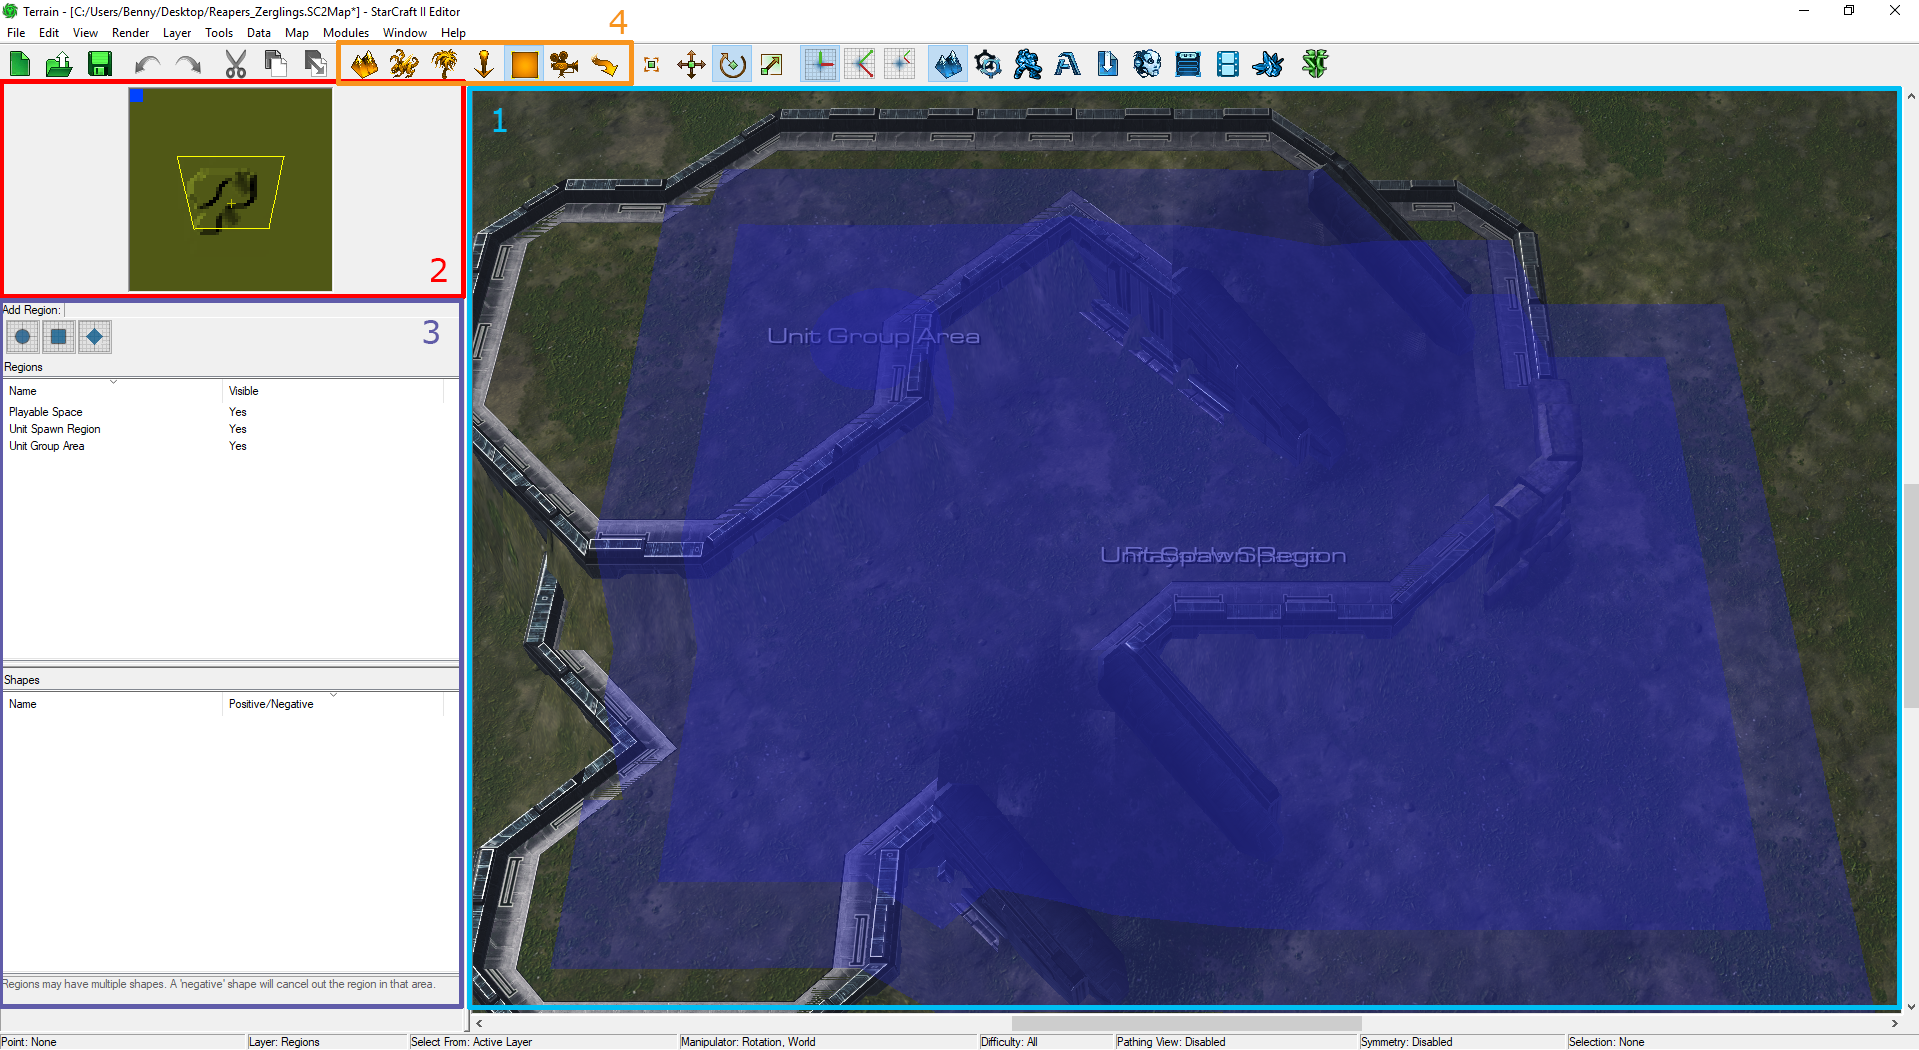
\includegraphics[width=1\textwidth]{Figures/Editor_bordered.png}
  \caption{The StarCraft II Map Editor User Interface}
  \label{fig:editor-general}
\end{figure}
Figure \ref{fig:editor-general} shows the user interface upon opening the StarCraft II Map Editor.
The cyan bordered window is the main view, that controls very similar to a 3D modelling program. It shows the entire map with a camera that can be moved and rotated, and additional information depending on the active view type chosen with the buttons bordered in orange. There are different layers available for viewing and manipulating different components like terrain, textures, units, scenery, or, active in the screenshot, game regions. Bordered with red is the minimap view of the map that gives a full 2D representation of the map, and bordered in purple are the available options for the active tool. Most tools work similar to a 2D Brush with which the surface of the map is painted.


\subsection{Triggers}
\begin{figure}[htb]
  \centering
      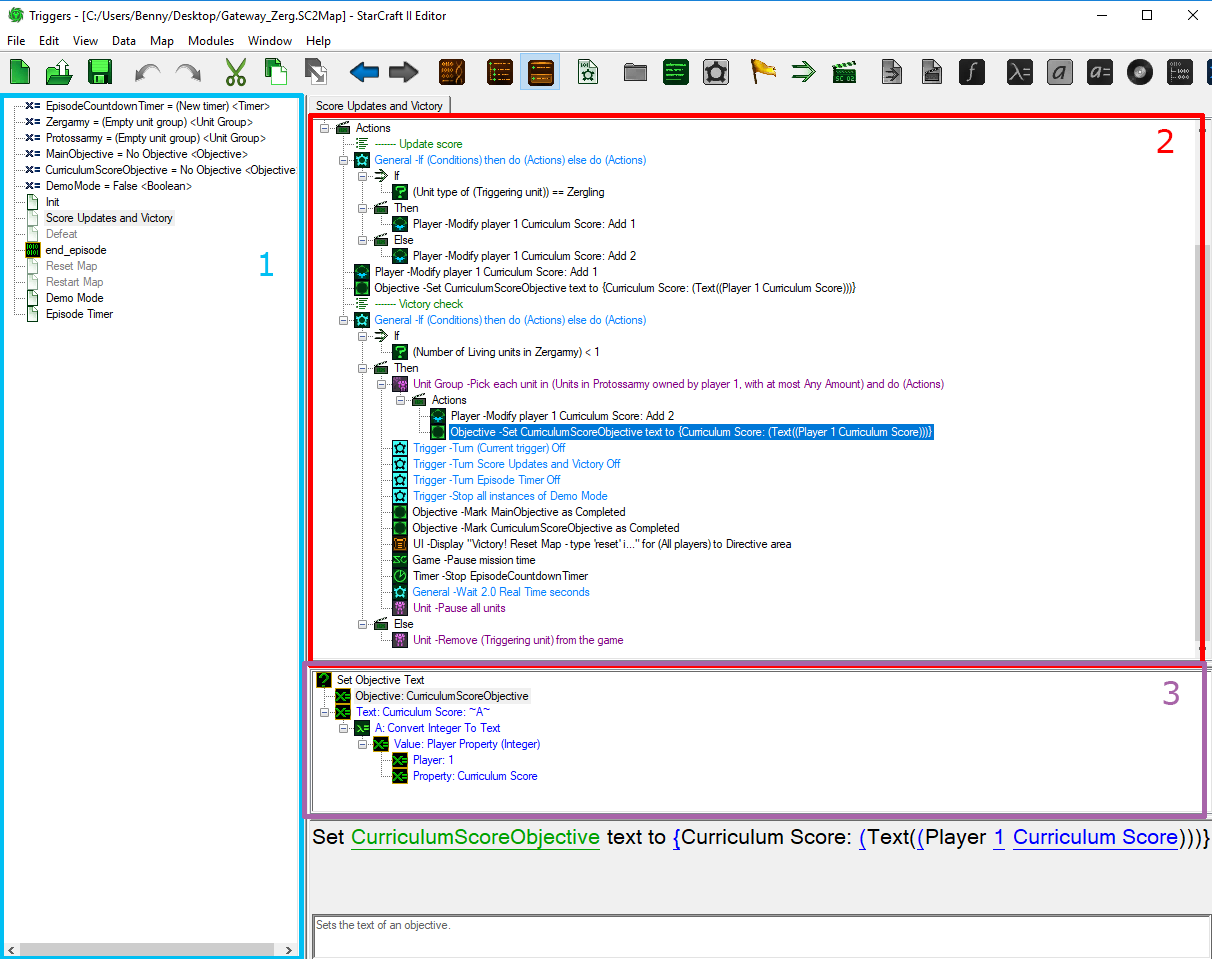
\includegraphics[width=1\textwidth]{Figures/Triggers_bordered.png}
  \caption{The StarCraft II Map Editor Trigger Module Interface: 1 - Overview of all Map Triggers and Global Variables, 2 - Trigger blocks of currently viewed trigger, 3 - Options of currently selected trigger block}
\end{figure}
The "Triggers" Module of the StarCraft II Map Editor is where the actual game logic of the map is created. It functions similar to a programming language, and many familiar concepts like for and while loops and conditionals can be found in this module, but instead of writing actual code, triggers work with predefined elements and functions that can simply be plugged into each other. There is also the option to write custom code using the galaxy code scripting language, but as the predefined functions available are very extensive this was not necessary in this project.

Trigger blocks can be divided into three main categories: Events, Conditions, and Actions.
Events are what causes a trigger to run. Some examples are "If any unit dies" or a periodic event like "Every x in-game seconds". Conditions are the familiar if, for, while etc. statements that handle control flow in a trigger, and actions are all other, regular statements.

Each trigger inherently has four categories to place trigger blocks in. Events, Local variables, Conditions and Actions. Only the Events category is strictly required to have one or multiple elements placed in it, and these decide, when the trigger is activated. The Conditional category only accepts trigger blocks of type condition. These conditions are tested when one or more events in the Events category fire to further determine whether to run this trigger. The Action category then holds all Trigger blocks, that are run in order after all conditions in the conditional category are met. The Local Variables category simply allows the creation and initialization of private variables that will only be accessible inside of this trigger.

\subsubsection{Galaxy Code and Trigger Debugging}
Before execution all trigger blocks are converted into StarCraft II's own scripting language Galaxy Code. The StarCraft II Map Editor also comes with a comprehensive debugging suite, that deals with Galaxy Code directly, and not with triggers. As the translation of trigger blocks into Galaxy Code is not always straightforward and there is substantial amounts of boilerplate code for every map, debugging can be considerable more challenging than the actual trigger blocks might indicate.


\subsubsection{Example Trigger Code}
While each scenario requires somewhat unique triggers, there is considerable overlap in the basic setup. This section will go through one example of all the triggers necessary for such a scenario with pointers to some of the differences between the scenarios.

The first Trigger that is common between all scenarios is the Init Trigger, that is automatically run after the map is first initialized.
It starts off with a group of trigger blocks that set up the camera and the playable space of the map. Since these scenarios feature only a small play area of a single screen, the playable area is restricted to this region. Doing that prevents units from moving outside of this region, and commands that are targeted outside this region are instead targeted to the closest point within this region.

Next, the camera of player 1, which will be controlled by the algorithm, is centered on this area and then locked in place, to make sure the player/algorithm can instantly begin the scenario without the need for screen panning, and cannot accidentally pan the screen during play. Lastly, the fog of war is removed to ensure visibility of the entire area, even uphill and if friendly units would not ordinarily give vision.

\begin{figure}[htb]
  \centering
      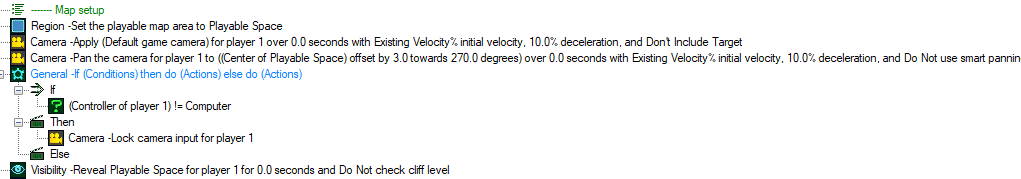
\includegraphics[width=1\textwidth]{Figures/Triggers/trigger_init_scenario.png}
  \caption{ Init Trigger: Camera and Play area setup }
\end{figure}

The next group of blocks inside the Init trigger sets up the units and upgrades needed for the specific scenario. This is substantially different for each scenario. This example uses two spawn regions, Left and Right which either spawn enemy or friendly units. Which region spawns which type of unit is chosen at random. This is done in order to give the environment some more randomness.

\begin{figure}[htb]
  \centering
      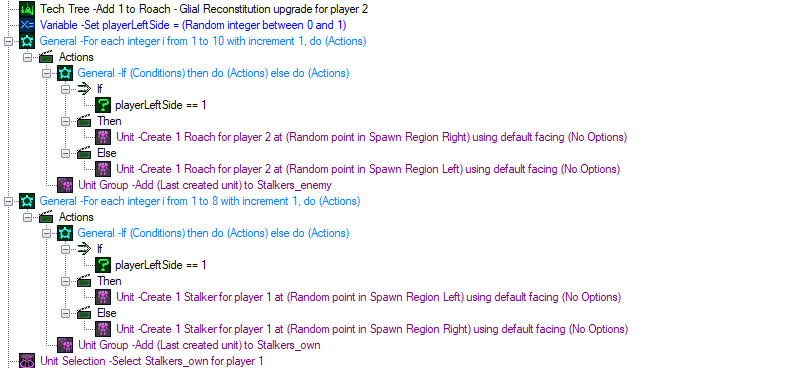
\includegraphics[width=1\textwidth]{Figures/Triggers/trigger_init_units.png}
  \caption{ Init Trigger: spawning of units }
\end{figure}

A different approach is chosen for example by the Reapers vs Zergling scenario. In that scenario no specific spawn regions are set, and instead all units of a group are spawned on a single point taken randomly from an area roughly the size of the playable area. Before spawning, it is ensured, that the two spawn points are not too close together, as that would interfere with the scenario.

The last part of the Init Trigger then sets the score, objective and an episode timer, that determines when the episode automatically ends. An episode timer is incorporated even in scenarios that are not time based simply in order to set a maximum episode length and prevent infinitely long episodes.

\begin{figure}[htb]
  \centering
      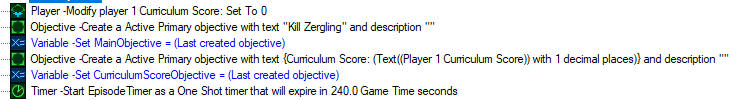
\includegraphics[width=1\textwidth]{Figures/Triggers/trigger_init_timer.png}
  \caption{ Init Trigger: Score variable and Episode Timer }
\end{figure}

The next trigger that is common between all scenarios is the Victory Trigger, that is responsible
for updating the score and checking whether a victory condition is met. This trigger usually activates using the "Any Unit dies" Event. A conditional then tests, what player the dying unit belonged to and, if multiple unit types are used for this scenario, which unit type it is. After that is determined the score is updated accordingly.

\begin{figure}[htb]
  \centering
      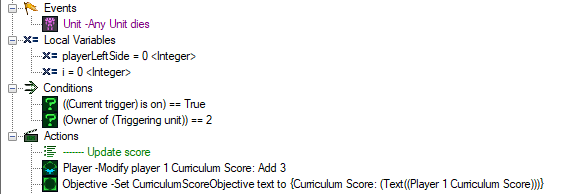
\includegraphics[width=1\textwidth]{Figures/Triggers/trigger_score_update.png}
  \caption{ Victory Trigger: Updating the score }
\end{figure}

The second part of the trigger then uses a conditional to check whether victory has been achieved yet. Most of the time that is the case if all enemy units have been defeated. Is Victory achieved, this trigger effectively pauses the game by stopping all active triggers, timers, units and the mission time. Additionally the objectives are set to completed, which signals pysc2 that an episode is completed and "reset" should be written to chat to activate the Reset Trigger, which resets the environment for a new episode. Depending on the scenario the defeat is handled either with a very similar trigger to that of the victory trigger or, in simple cases as a subconditional inside of the victory trigger.

\begin{figure}[htb]
  \centering
      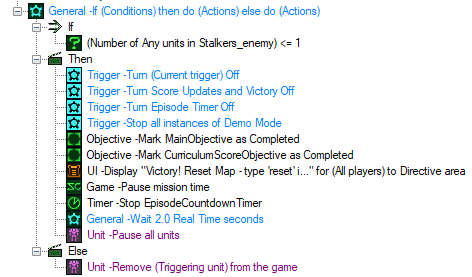
\includegraphics[width=0.8\textwidth]{Figures/Triggers/trigger_score_victory.png}
  \caption{ Victory Trigger: Checking the victory condition }
\end{figure}

The Reset trigger first of all stops all episode relevant timers and triggers. Although this should have already be done by victory or defeat triggers, this is repeated here. This is mainly for mid-episode resets, for example for debugging purposes. Additionally, all units are entirely removed from the game.

\begin{figure}[htb]
  \centering
      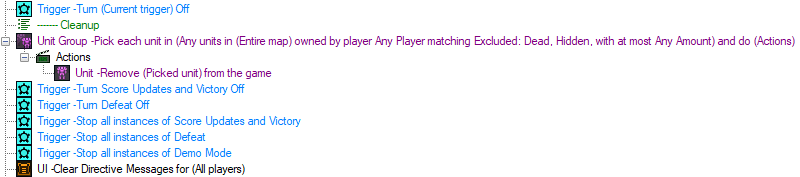
\includegraphics[width=1\textwidth]{Figures/Triggers/trigger_reset_stopall.png}
  \caption{ Reset Trigger: Checking the victory condition }
\end{figure}

After that follows the resetting of all global variables used during the episode and the re spawning of units.
Unfortunately there is no easy way to simplify this. Therefore the code is very similar to the code used in the Init Trigger. Unit upgrades do not have to be reapplied here, as they are valid until the map is fully closed.

\begin{figure}[htb]
  \centering
      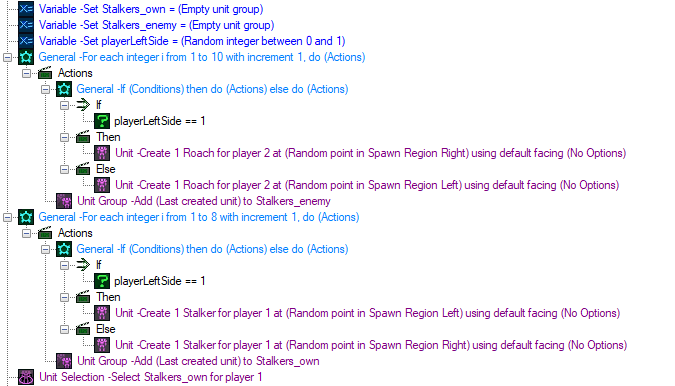
\includegraphics[width=0.8\textwidth]{Figures/Triggers/trigger_reset_resetvars.png}
  \caption{ Reset Trigger: Resetting variables }
\end{figure}

Lastly, the reset trigger re activates all triggers and timers needed for the episode and if applicable gives orders to the units that will not be controlled by player 1.

\begin{figure}[htb]
  \centering
      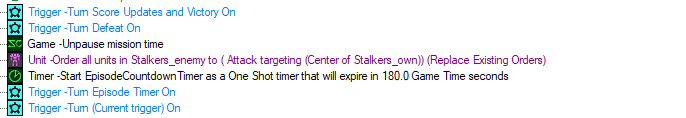
\includegraphics[width=0.8\textwidth]{Figures/Triggers/trigger_reset_turnon.png}
  \caption{ Reset Trigger: reactivating triggers }
\end{figure}

The last trigger that all scenarios share is the Restart trigger. This is a very simple trigger only needed for debugging, or when the maximum number of steps allowed for a map is reached during training. A maximum number of steps is enforced mainly to prevent memory problems.
It simply reinitialises the map, which effectively restarts the entire environment. 
This reinitialization is very slow however, and should therefore not be used in place of the reset trigger, and only if necessary.
After reloading the map the Init Trigger is executed again, and the scenario starts fresh.

\begin{figure}[htb]
  \centering
      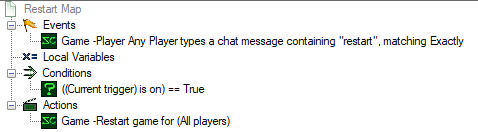
\includegraphics[width=0.6\textwidth]{Figures/Triggers/trigger_reset_full.png}
  \caption{ Restart Trigger }
\end{figure}



\subsection{Altering Game Data}
The "Game Data" Module allows the adjustment of many different game variables. Here one can change unit and building properties, terrain characteristics and even parameters of the unit behavioural AI. In this project this module was mainly used as a means to tune the difficulty of a scenario. For the "Find Ultralisk" and "Find Ultralisk With Creep" in particular it was important to keep them as easy as possible while still maintaining an interesting challenge.
To that effect multiple variables of the friendly unit were altered:
\begin{itemize}
\item Movement Speed - The Movement Speed was slightly increased in order to decrease the amount of steps needed towards the enemy unit.
\item Weapon Range - To counteract the previous change somewhat the range was decreased. This means that while it overall takes less steps to reach the target, it has to be reached more accurately.
\item AI Target Leash Acquiring Range + AI Target Leash Reaquiring Range - Both of these variables relate to the unit AI that every unit has built into it, regardless of whether it is controlled by a human or AI. The unit AI handles mostly pathfinding and one of the features of this unit AI is that if a unit is close to but not in range of an enemy unit it will "leash" to it. meaning that it will automatically move to attack it and all further attack move commands that do not target a specific unit will be voided. While useful in the normal game this feature would heavily distort the outcomes of the tests. For that reason these two ranges were set to 0 effectively disabling this feature.
\end{itemize}

\subsection{RL Specific}
For a map to be properly usable with PySC2 there are a few behaviours that have to be implemented.
The first one is the reward system. Without it, the only reward available in PySC2 is either a 1 or a 0 depending on whether the agent won or lost the game. Giving more nuanced rewards during an episode is done by manipulating the cumulative score. In StarCraft II's multi-player the cumulative score is a loose indicator of how well a player did, aggregating points for gathered and spent resources, army value etc.. Using the map editor however it can be arbitrarily set using triggers, allowing for various reward policies to be implemented. This cumulative score is send directly to the PySC2 environment with each step as the reward.

The second behaviour is the reset and restart handling. Resets are supposed to happen after each episode and revert the environment back to the state at the start. PySC2 sends the reset signal by having the agent type "reset" in the in-game chat. An event trigger has to listen to this in-game message and by hand reset each part of the environment. Similarly the restart signal is sent by typing "restart". 

\section{Scenarios}
\label{sec:scenarios}
Instead of using the "Mini Games" provided with PySC2 I wanted to build my own scenarios, both to build scenarios that are more in line with the specific topic of this thesis and more importantly to have more control over what exactly the challenges in the scenarios are.
Furthermore, most of these "Mini Games" are very artificially constructed and only have a very peripheral relation to the actual game of StarCraft II. While some of the scenarios in this project are abstract as well, three scenarios were created, that reflect actual combat scenarios that occur very frequently in competitive play.

What all of these scenarios have in common, is that they use an arena style map that is at most as big as one screen's field of view. This eliminates the need for screen panning, which would add an enormous amount of complexity to the scenarios.
Also, all of these scenarios pit the reinforcement learning agent against either a static environment, with hard coded enemy unit behaviour, or the built in AI.
The next sections will give a brief description of each scenario and what the agent was expected to learn from the environment. Also there are videos on the accompanying usb drive of each scenario being solved by one of the reinforcement learning algorithms, and also by a human should their strategies differ greatly. The strategies depicted in these videos are further discussed in chapter \ref{chap_eval}

\subsection{Find Ultralisk}
\begin{figure}[htb]
  \centering
      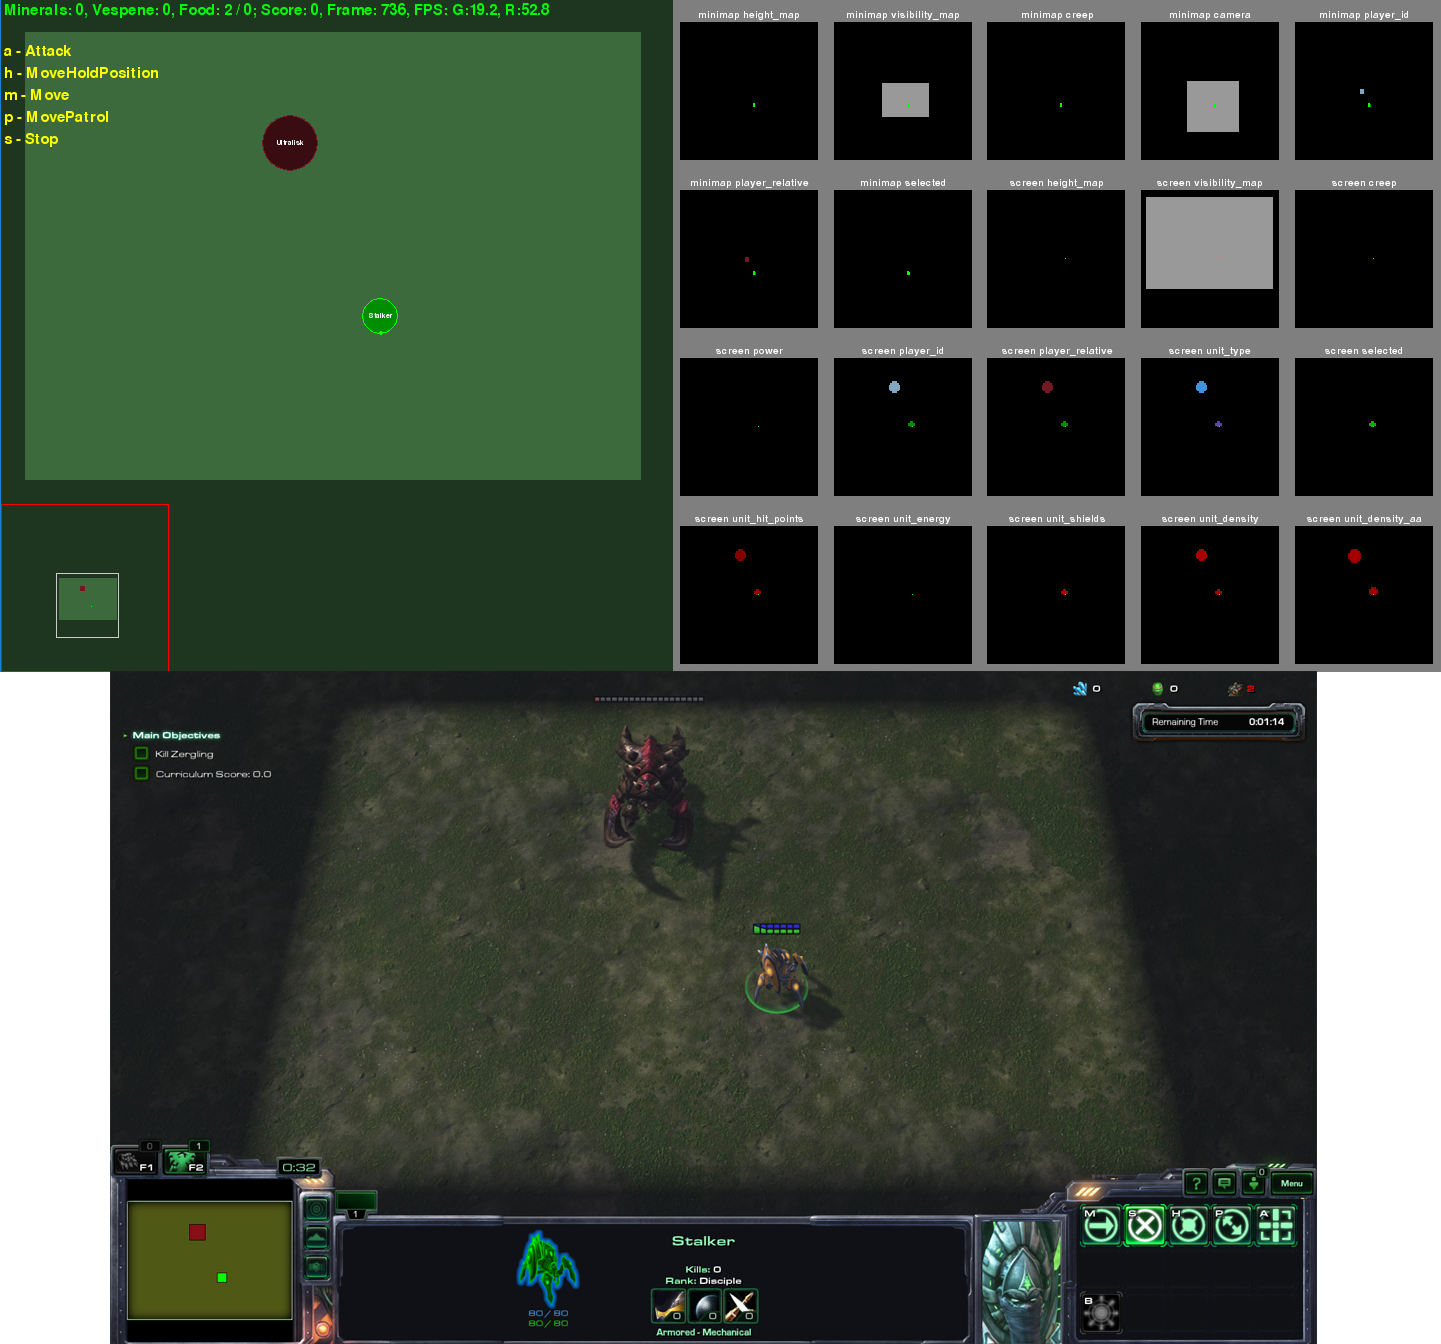
\includegraphics[width=0.8\textwidth]{Figures/FindUltralisk.png}
  \caption{PYSC2 debugging view(top) and ingame view(bottom) of the FindUltralisk Scenario. Important Feature Layer: screen\_player\_relative }
\end{figure}
The Find Ultralisk scenario can be considered a "Hello World" scenario. It was created with the intention of being as easy as possible. As a result, this scenario is mainly used to verify whether a reinforcement learning algorithm actually works. Essentially it is very similar to the "MoveToBeacon" Mini Game, that is provided with PySC2, but is a combat scenario variant of it. This scenario features one ranged unit controlled by the RL agent, one static enemy melee unit and an otherwise empty map. The Ultralisk was chosen as the enemy unit, as it is very big, and should therefore be especially easy to detect for the CNN.

Both units get spawned at random positions within the arena which are at least 7 units of distance apart from each other at the start of each episode.
The objective for the agent is to move it's unit in range to the Ultralisk and attack it. After one attack the Ultralisk dies which awards the Agent with 1 reward score.
After that, a new Ultralisk instantly spawns at a random point, again at least a distance of 7 away from the current position of the agents unit. This continues, until the scenario ends after 240 timesteps. Thus, the faster the agent manages to kill the Ultralisks, by moving towards them in the most direct and efficient way possible, the higher the episodic reward.

Using the environment wrappers depicted in section \ref{sec:wrappers}, two versions of this scenario were created. The simplified version makes use of only four actions for moving the unit up, down, left, or right. The environment wrapper then translates these actions into an attack\_screen action with screen coordinates that are shifted a distance of 5 from the current unit position in the respective directions.
In order to get by with only these four actions the unit has to be preselected in each episode, which is done through the map editor.
The advanced version directly uses the attack\_screen command with screen coordinates chosen by the neural net, and for additional complexity the no\_op command, which simply does nothing, and the select\_army command, selecting all units a player owns.

\subsection{Find Ultralisk With Creep} 
\begin{figure}[htb]
  \centering
      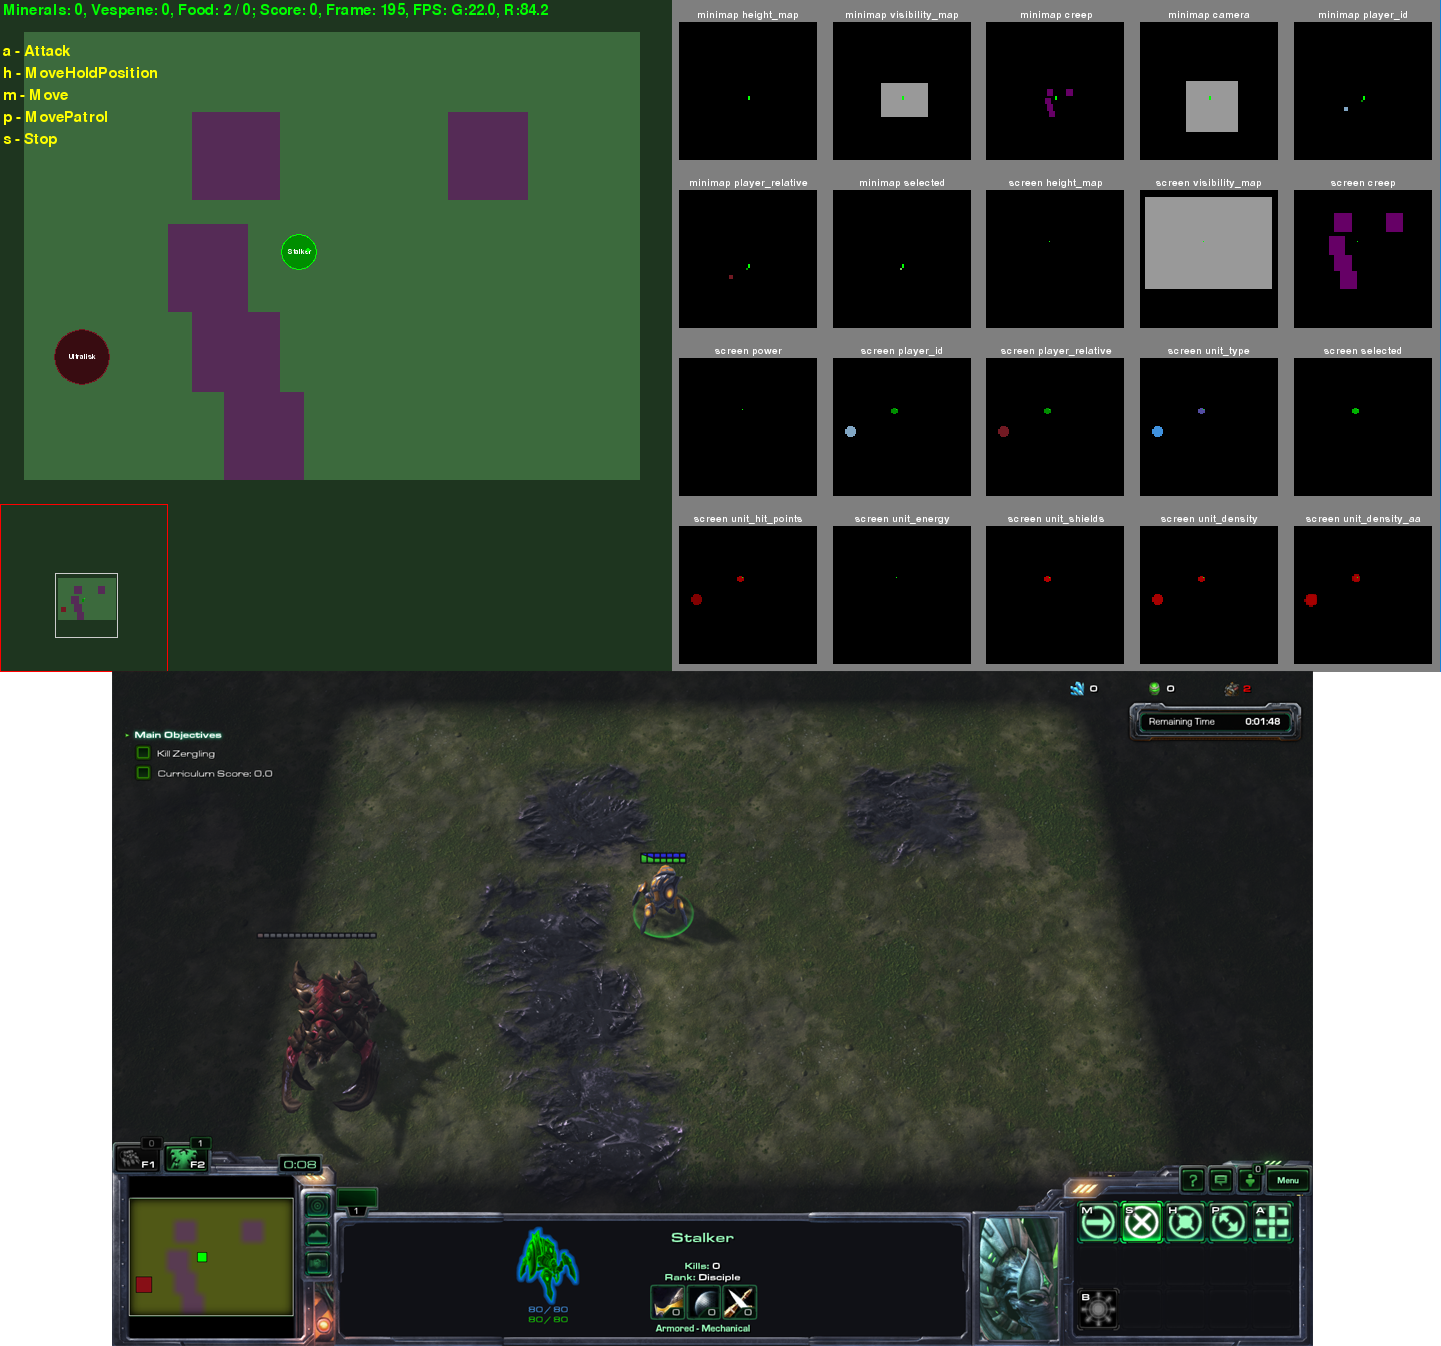
\includegraphics[width=0.8\textwidth]{Figures/FindUltraliskWithCreep.png}
  \caption{PYSC2 debugging view(top) and ingame view(bottom) of the Find Ultralisk With Creep Scenario. Important Feature Layers: screenplayer\_relative, screencreep }
\end{figure}

This scenario is a modification of the "Find Ultralisk" scenario described in the last section. Everything stays largely the same the only addition being "creep" surfaces. These surfaces are spread randomly across the arena and do not change locations until an episode is over. While largely harmless in the real StarCraft II game, in this Scenario these surfaces instantly kill the agents unit if it steps on them. This immediately ends the current episode and deducts 1 reward point. Accordingly the agents primary priority should be to stay alive, with actually killing Ultralisks and gaining rewards becoming only the second priority. This scenario also has the same simplified and more challenging variants as the Find Ultralisk scenario.

\subsection{Blink Stalkers vs Roaches}
\begin{figure}[htb]
  \centering
      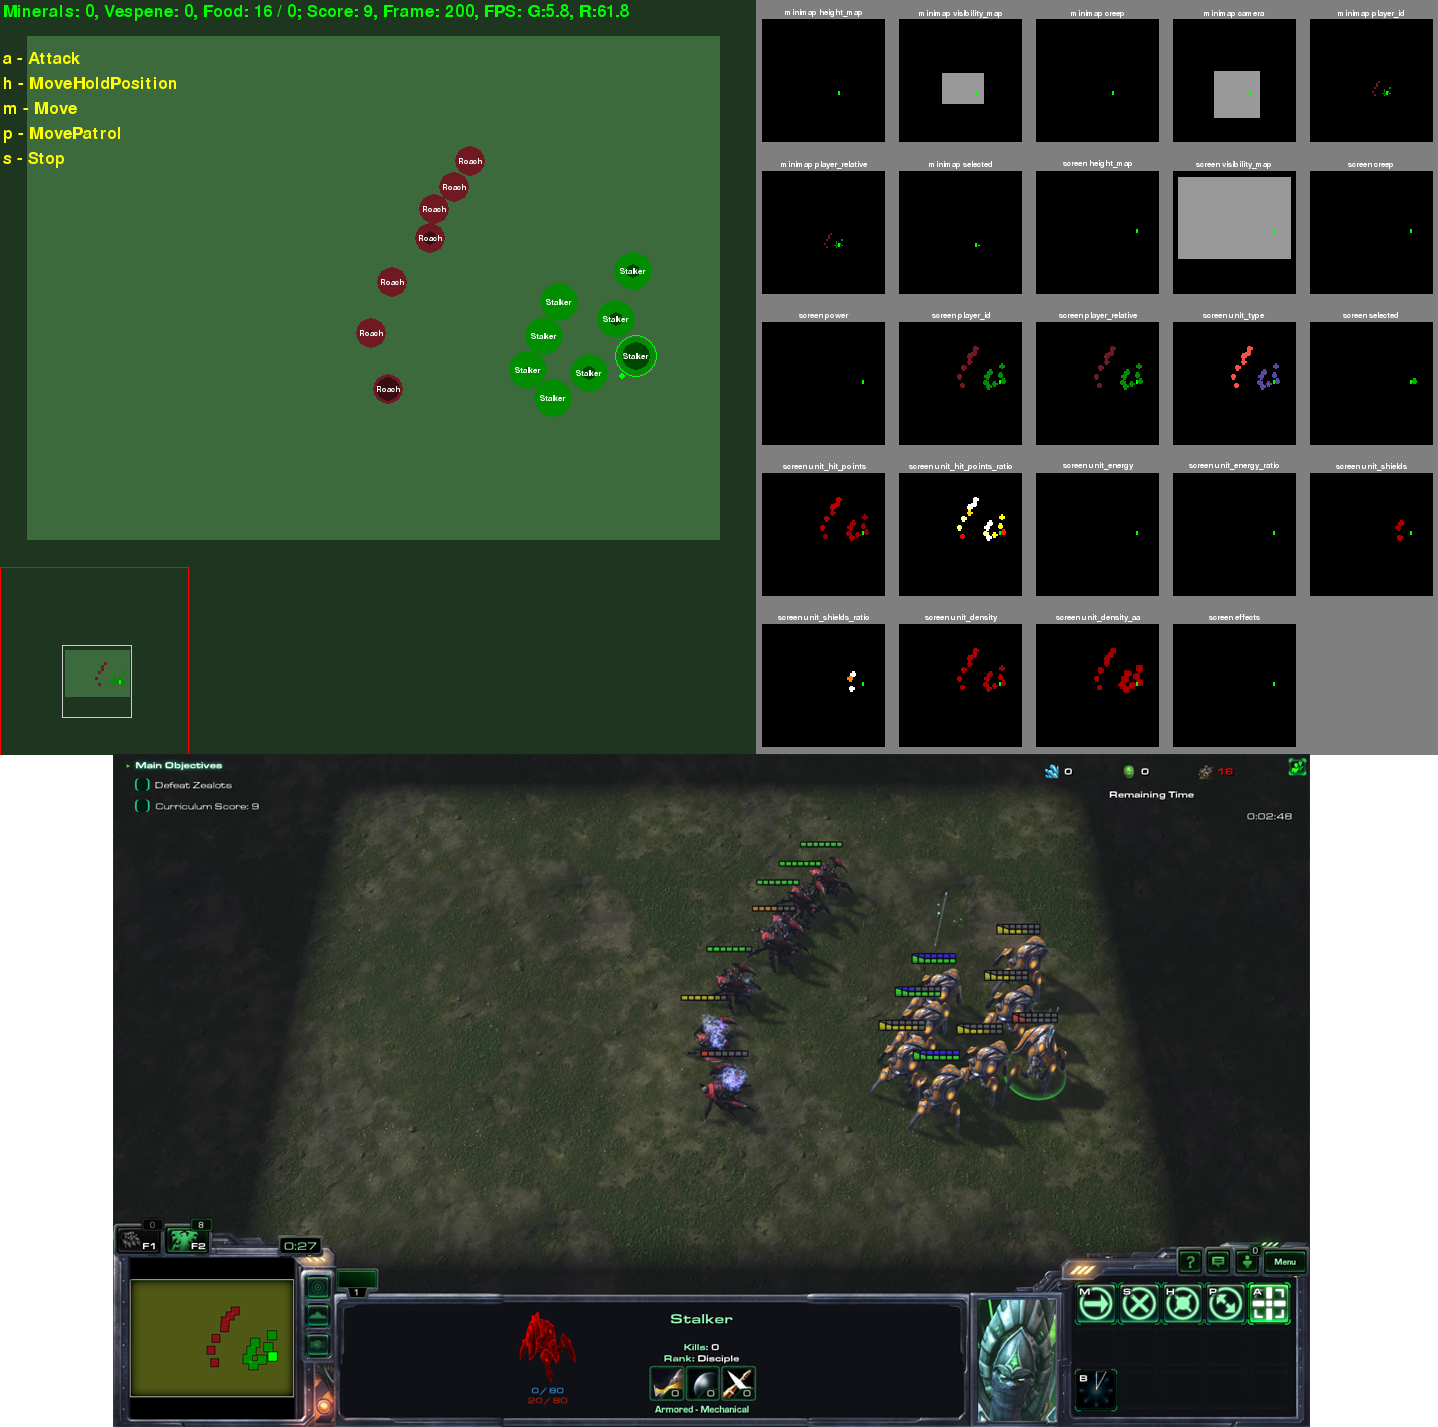
\includegraphics[width=0.8\textwidth]{Figures/StalkersRoaches.png}
  \caption{PYSC2 debugging view(top) and ingame view(bottom) of the Blink Stalkers vs Roaches Scenario. Important Feature Layers: screenplayer\_relative, screenselected, screenunit\_hit\_points, screenunit\_hit\_points\_ratio }
\end{figure}

"Blink Stalkers vs Roaches" is the first scenario that is taken directly from the competitive 1vs1 mode of StarCraft II. In this scenario two similar, but imbalanced armies fight each other. The army that will be controlled by StarCraft II's builtin AI contains 10 Roaches, a Roach being a basic ranged unit. The army controlled by the RL algorithm contains 8 Stalkers, a similar ranged unit that has slightly longer range and also has a "Blink" ability unlockable via research.
This scenario arises quite often in Protoss vs Zerg match-ups, as Roaches and Stalkers are 2 of the most integral units of their respective races.

"Blink" is an ability that allows a Stalker to instantly teleport to a location nearby. Using the "Blink" ability a Stalker army can become much more efficient. The strategy that works best is to always teleport Stalkers that only have little health left to the back of your army. If done correctly, the teleported Stalker should still be close enough to the enemy that it walks back into the fight on its own, but far enough away, that enemy units no longer attack it. Because the built in AI does not intentionally focus on low health enemies, teleported Stalkers can stay much longer in the fight even though they are close to being destroyed. The numbers of units for both sides were chosen such that if the RL algorithm does not learn this strategy it will lose the battle every time, and if it executes this strategy perfectly it should win every time without losing any Stalkers of its own.

For this scenario there is an immediate reward of 1 point every time an enemy Stalker dies, and also an additional end of episode reward of 2 for each Stalker belonging to the RL algorithm that is still alive.

The feature layers used for this scenario are player\_relative, selected, and hit\_points.
Available as actions are the "Blink" action and the "Select Point" action, both requiring screen coordinates as parameters. For this scenario there is no easy variant.

\subsection{Gateway Army vs Zerglings}
\begin{figure}[htb]
  \centering
      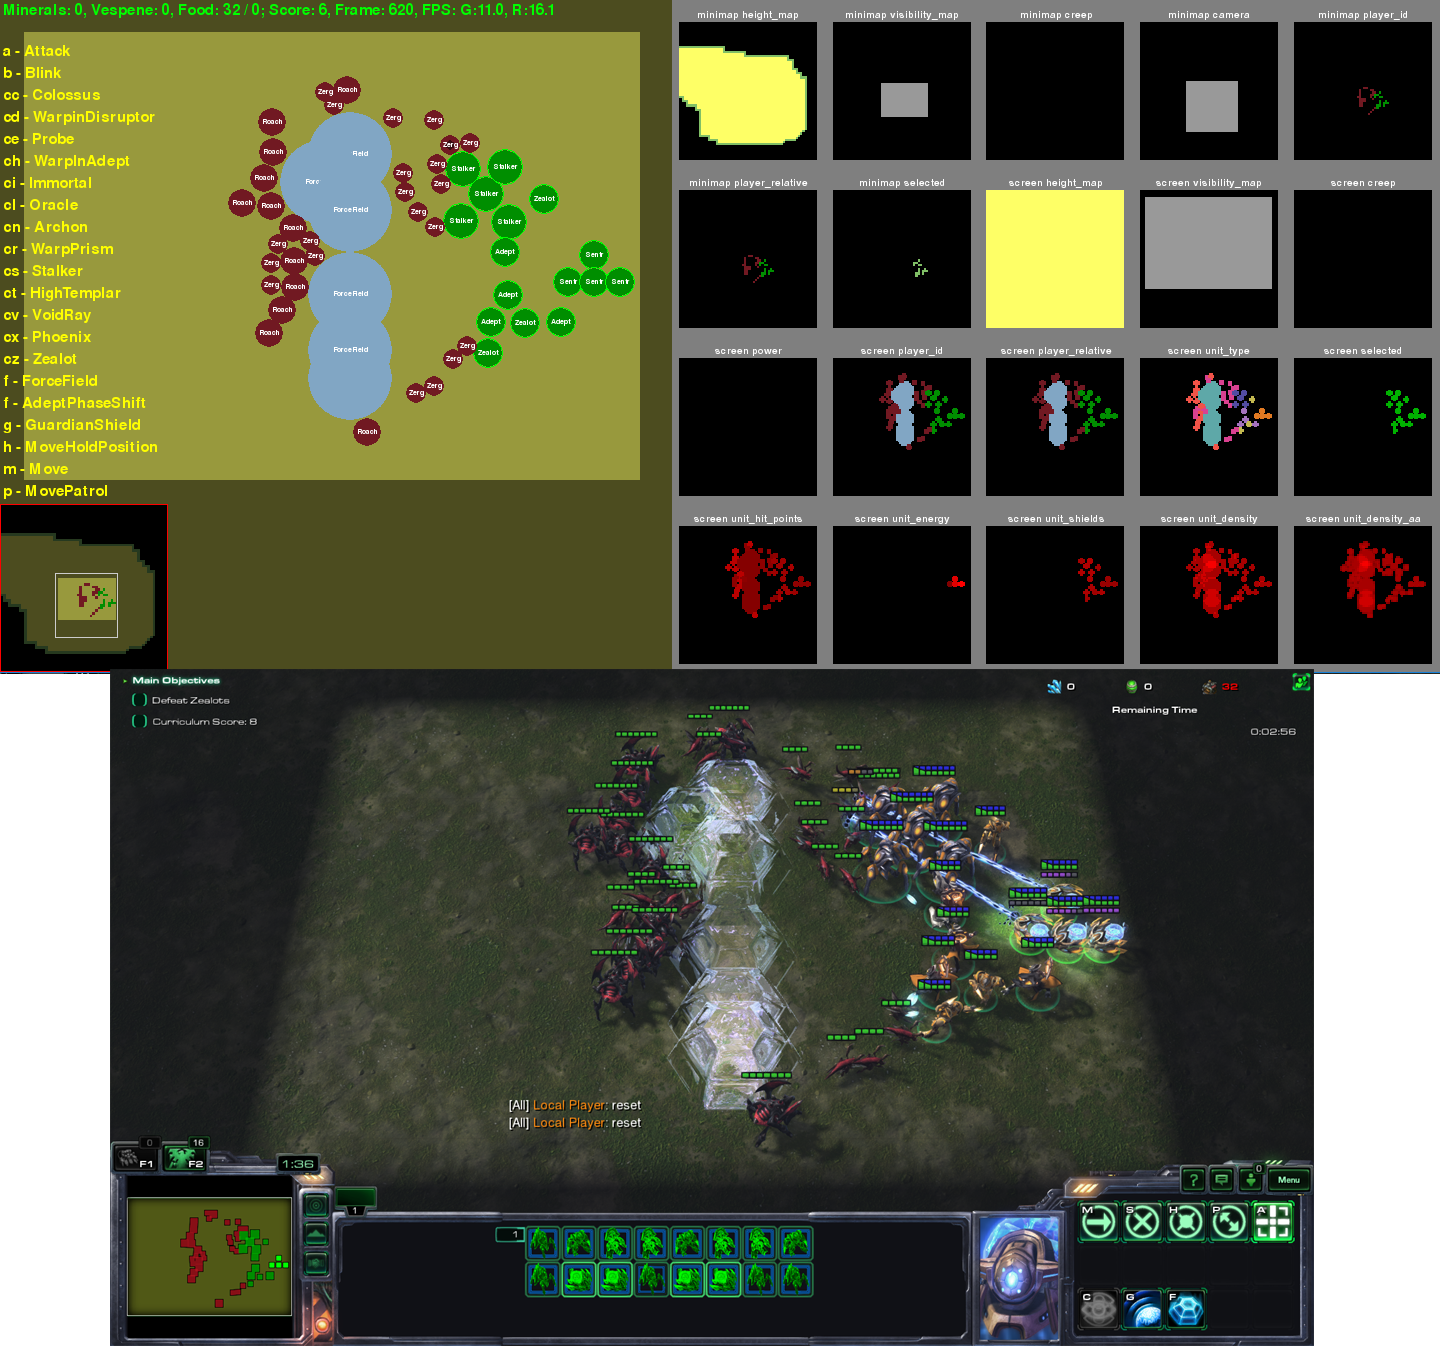
\includegraphics[width=0.8\textwidth]{Figures/GatewayZerg2.png}
  \caption{PYSC2 debugging view(top) and ingame view(bottom) of the Gateway vs Zerg Scenario during the fight, after some Forcefields and Guardian Shields were used. Forcefields show up as neutral units and can be seen influencing the battlefield, while Guardian Shields can not be seen any of the input layers, which is either a Bug or missing feature and makes their use by the AI questionable. }
\end{figure}

This scenario is again a very common combat scenario from the competitive mode of StarCraft II.
It pits a standard Protoss Gateway army consisting of Zealots, Stalkers, Sentries and Adepts controlled by the RL algorithm against a tier 1 Zerg army of Zerglings and Roaches. 

The most important unit for this scenario is the sentry. It has two abilities: Forcefield and Guardian Shield. Forcefield is an ability that costs 50 energy of the Sentry's 200 maximum energy to create a forcefield on a specified location that lasts for 11 seconds and that both enemy and friendly units can not pass through. Using multiple Forcefields it is possible to effectively cut the enemy army in half, so that you can fight them separately, which is much easier and more effective. Guardian Shield costs 75 mana and constructs a shield around the sentry and nearby units that reduces all incoming ranged damage by two. Management of those two abilities is paramount to the success in this Scenario.

As input layers player\_relative, hit\_points, and unit\_type were used. The actions for this scenario are attack\_screen, forcefield, which both require screen coordinates and also guardian\_shield.


\subsection{Reapers vs Zerglings}
\begin{figure}[htb]
  \centering
      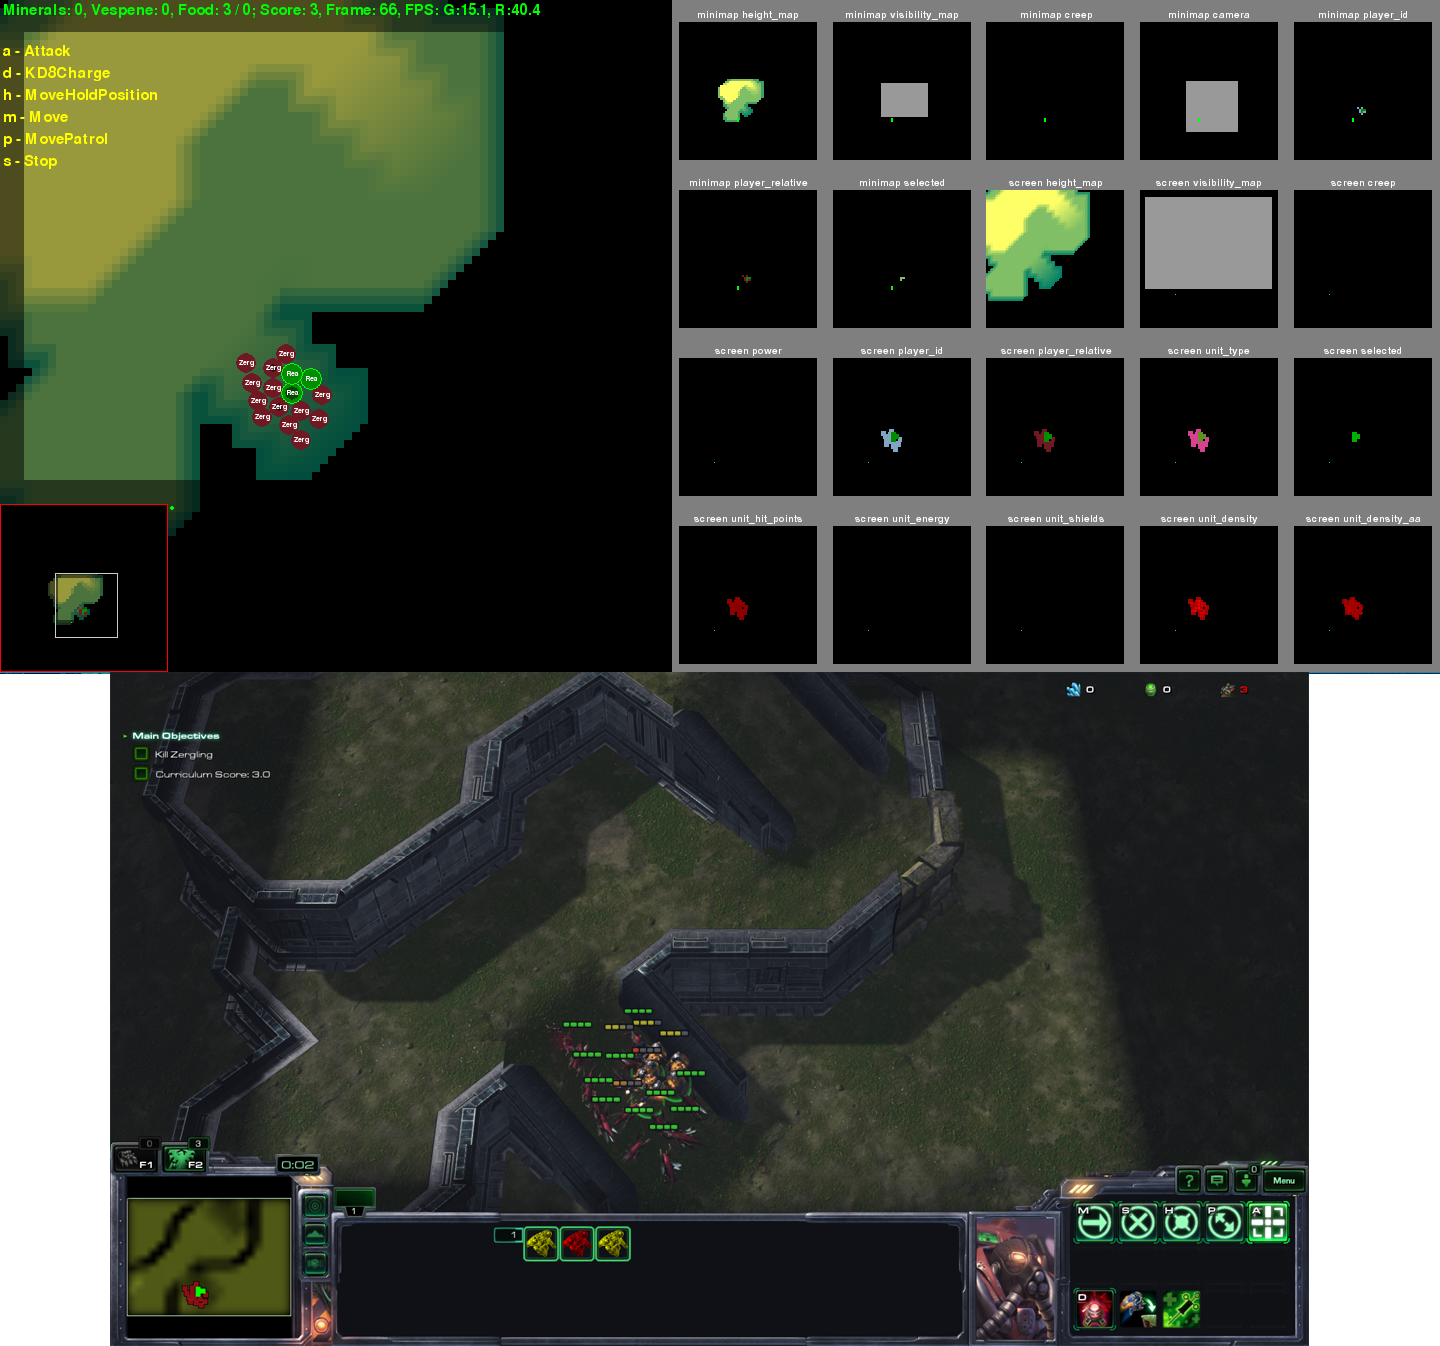
\includegraphics[width=0.8\textwidth]{Figures/Reapers_zergling.png}
  \caption{PYSC2 debugging view(top) and in game view(bottom) of the Reapers vs Zerglings Scenario }
\end{figure}
This scenario features a small version of a very popular opening in the Terran vs Zerg matchup.
It is also the first scenario to feature terrain with different levels of height, that the algorithm can use to it's advantage. The Reaper is a very unique ranged unit with the passive jetpack ability, that allows it to jump up and down cliffs. Zerglings being a melee unit cannot attack enemies above or below them so their only option to get to and attack the agents units is to use the ramps that connect the different levels of height in the terrain.

The input layers for this scenario are player\_relative, hit\_points and height\_map. The actions are move\_screen and attack\_screen both requiring screen coordinates as parameters. For this scenario there is an easy variant, that uses only eight actions: four variants for the directions up, left, right and down for each of the 2 actions.


\subsection{Failed Attempt: Vulture vs. Firebats}
\label{sec:failed}
The first attempt at a reinforcement learning scenario was to recreate a similar scenario as in the paper \citep{broodwarRL}.
In this scenario the RL algorithm controls a single fast moving ranged unit which fights a group of slower moving and lower range or melee units. The best strategy here is to kite the enemy group by shooting and fleeing in an alternating manner. This keeps the agents unit out of the range of the enemy units and with ideal execution it is possible to defeat all enemies without ever getting hit.

Like in the aforementioned paper this was supposed to be solved in a very simplified manner using only two actions, attacking and fleeing. These actions were implemented much more simplistically however. In this project the attack action simply executes an attack move command on the coordinates of the closest enemy, while the fleeing action calculates a vector that is opposite to the attack vector. Should the escape vector lie outside of the playable area it is rotated until it is fully inside. The programming of these two actions was kept intentionally very simple, because they have to be calculated in every step. This sacrifices some accuracy in favour of faster computation and training. Nevertheless this was one of the major problems with this scenario. The hard coded actions simply were either too slow or too inaccurate to be suitable for training with. The other problem was, that it is not possible to determine the state (moving, attacking, etc.) of a single unit at any given time using the StarCraft II API. For the kiting strategy required in this scenario, this would be invaluable information. \citep{broodwarRL} alleviated this challenge somewhat by setting the time between agent steps to how long one attack action would take. 

While also possible in this project it was felt, that all scenarios should share as much common ground as possible and this was too arbitrary of a modification to make and would not necessarily give valuable comparisons to other scenarios. Because this Scenario was supposed to be the easiest, and entry scenario for this project and these challenges presented themselves as non-trivial this scenario was ultimately abandoned and replaced by the much simpler and straightfoward Find Ultralisk scenario.   

\subsection{Summary}
\begin{landscape}
\begin{table}[htb]
\centering
%\resizebox{\textwidth}{!}{%
\begin{tabular}{p{2cm}p{3cm}p{3cm}p{3cm}p{2cm}p{1.5cm}p{1.5cm}p{2cm}p{2cm}}
%\begin{tabular}{@{}lllllllll@{}}
\toprule
Scenario               & Available Actions                                                         & Available Actions (Simplified) & State Layers                                                                             & Estimated Difficulty (0 - 10) & Min Reward  & Max Reward & Novice Human score & Expert Human score \\ \midrule
Find Ultralisk          & 7056 (Move\_Screen)                                                       & 4 (Up, Down, Left, Right)     & 1 (Player\_Relative)                                                                     & 0           & 0           & $\sim$50   & 45                     & 48                       \\  \addlinespace[0.35em]
Find Ultralisk With Creep & 7056 (Move\_Screen)                                                       & 4 (Up, Down, Left, Right)     & 2 (Player\_Relative, Terrain\_Creep)                                                     & 3     & 0           & $\sim$45   & 37                     & 42                       \\ \addlinespace[0.35em]
Reapers Zerglings       & 14112 (Move\_Screen, Attack\_Screen) + 2 (No\_op, Select\_Army)           & 8 (Attack UDLR, Move UDLR)    & 3 (Player\_Relative, Unit\_Health, Height\_Map)                                          & 6         & 0           & 19         & 17.5                   & 19                       \\ \addlinespace[0.35em]
Gateway Zerg            & 14112 (Forcefield\_Screen, Attack\_Screen) + 2 (No\_op, Guardian\_Shield) &                               & 6 (Player\_Relative, Hit\_Points, Hit\_Points\_Ratio, Unit\_Type, Energy, Energy\_Ratio) & 7            & $\sim$42(0) & 120        & 63                     & 99                       \\ \addlinespace[0.35em]
Stalkers Roaches        & 14112 (Blink\_Screen, Attack\_Screen) + 1 (No\_op)                        &                               & 5 (Player\_Relative, Hit\_Points, Selected, Unit\_Type, Hit\_Points\_Ratio)              & 10       & -10         & 100        & 60                     & 90                       \\ \bottomrule
\end{tabular}%
%}
\caption{Summary of key data points comparing the different scenarios}
\label{table:scen_summ}
\end{table}
\end{landscape}

This table \ref{table:scen_summ} gives a summary and comparison of some of the key data pertaining to all the scenarios previously discussed. The numbers in the available actions column assume a vertical and horizontal feature layer resolution of 84 pixels. The minimum and maximum rewards for a scenario can not be determined accurately in all cases. For the Find Ultralisk and Find Ultralisk With Creep scenarios for example, the maximum reward is somewhat dependent on the randomness of the spawns especially on the placement of creep patches which in rare cases restrict rewards almost entirely. Even in normal cases a deviation of ~3 points is likely for these two scenarios. 

For the Gateway vs Zerg scenario 0 and 120 are only theoretically the lowest and highest rewards resulting from killing no enemy units at all and eliminating all enemy units without losing a single unit respectively. Both of these are likely not actually achievable in game though. 42 is given as a secondary minimum reward for this scenario, as this is the lowest reward I was able to achieve when trying to purposefully sabotaging the win. 

The human baselines are average reward values over five runs with 1 practice run beforehand of one player, who has barely played StarCraft II at all (Novice) and a Master-ranked 1v1 player (Advanced), Master rank being the second highest rank after grandmaster and containing the 2\% best players of each continent. As these scenarios are simple enough, that even a novice player should be able to earn very high scores with a little practise these baselines were recorded only on a very sample size of the first few tries that the respective players had on these scenarios. 

\section{RL Framework}
\label{sec:rlfwork}
The following sections will discuss the general architecture of this project, how to run this project and all modules not directly pertaining to one of the reinforcement learning algorithms. Figure \ref{fig:proj} illustrates the project's architecture.
The train module handles the general setup and start of the reinforcement learning algorithms, the util module contains the helper module and the environment wrappers, that interface between the PySC2 environment and the reinforcement learning algorithms and the plot\_baselines module is a standalone module used for plotting the results of the training runs. There is also the semi standalone scenarios module, that is required by PySC2 to load the actual .sc2map files.


\begin{figure}[htb]
  \centering
      \includegraphics[width=1\textwidth]{Figures/Project_Overview.pdf}
  \caption{ Overview of the Project Architecture and module structure. The Train and plot\_baselines modules are the entry points for this project, with the train module starting one of the currently three available algorithms A3C, A2C and ACKTR and using one of the environment wrappers provided by the util.environments module}
  \label{fig:proj}
\end{figure}



\subsection{Setup}

The setup needed in order to run this project varies considerably depending on which method of providing the necessary dependencies is used. In all cases one needs to install one of the StarCraft II Clients available either on the Blizzard website for Mac/Windows builds, or the StarCraft II maschine learning API github repository for the linux client. PySC2 expects SC2 to be installed either in the home directory of the user or a custom location can be specified with the SC2PATH environment variable. 

If the tensorflow/keras code is desired to be executed on the GPU, which is highly recommended, one also needs to install current graphics drivers, the CUDA library and CUDNN. These can be supplied from either the systems' package manager or install files, or by anaconda. In the docker image they are already installed. Lastly, the python module dependencies are needed, all but one of which can be supplied by the python package manager pip.

The only non-pip module required is the OpenAI Baselines module available on Github. One thing to note is that at the time of writing the installation script provided with the baselines module breaks existing tensorflow-gpu installations and replaces them with the CPU only version. For this reason it is necessary to reinstall tensorflow-gpu afterwards. Finally, the .sc2map files located in the Maps folder of this project need to be copied into the \lstinline{Maps/rl_scenarios} directory of the StarCraft II installation.


\subsubsection{Docker}
\label{sec:docker}
In order to deploy and run this project on different machines as easily as possible a docker image was created. This became necessary in particular for running the project on the Datexis GPU cluster of the university, as the required libraries to build some of the python modules were not available on the fedora machine.

The Docker image is based on the tensorflow-gpu image, which in turn is based on one of the nvidia-docker images. On top of this tensorflow image installed are some additional programs like git and pip, and the required python modules. In addition the cudnn version was updated to version 6. In order to keep the image as small and portable as possible, the StarCraft II Client and the projects git repository are not included in the docker image and have to be downloaded separately.

Actually running this docker image involves first starting it as a daemon with the directory containing both the project code and the StarCraft II folder as a shared folder. This can be done using the command 

\begin{lstlisting}[language=bash]
nvidia-docker run -d --rm --name bwinter-tensorflow -v /data/home/$USER:/data/local/home/$USER bwinter-tensorflow:latest
\end{lstlisting}

Afterwards one can connect to the running image by executing a bash shell on it:
\begin{lstlisting}[language=bash]
nvidia-docker exec -it bwinter-tensorflow bash
\end{lstlisting}

When connected to the image one can navigate to the shared project directory and run it as normal.
\subsection{Usage}
There are two main entry points for this project: train.py and plot\_baselines.py.
The train.py module handles not only training, but also testing and validation of all algorithms, Baselines and A3C, used in this project. There are a couple of run option available in addition to the engine parameters mentioned in section \ref{sec:engparam}:
\begin{itemize}
\item map - Name of the map to be run
\item algorithm - path of the algorithm to be run. Has the format modulepath.Class.
\item run\_time - specifies either seconds(A3C) or number of steps(Baselines) that the algorithm should run for
\item threads - number of environments to run in parallel
\item save\_model - folder to save trained models in. No models saved if left empty
\item load\_model - model file to be loaded. only required for validation
\item render - whether to render the PySC2 debug window. Only recommend when running single environment (sim\_proc)
\item validate - whether to run validations instead of training. During validation the  model is not improved.
\item action\_args - whether to run environments with action coordinate arguments or simplified action lists.
\item lr - learning rate to be used
\item gamma - discount factor
\end{itemize}

A standard command for training could then for example be

\begin{lstlisting}[language=bash]
	python train.py --map FindUltralisk
    	--algorithm baselines_mod.acktr.acktr.Acktr
    	--run_time 80000000 --save_model models/fu
        --lr 0.0005 --action_args > logs/last.log 2>&1 &
\end{lstlisting}

The plot\_baselines.py module only has one parameter: dir. This parameter specifies the directory in which the environment logfiles can be found.

\begin{lstlisting}
python plot_baselines.py --dir logs/res_fu_acktr
\end{lstlisting}

\subsection{Train Module}
The train.py module is responsible for defining and initializing absl command line parameters, setting up logging, loading maps, and importing and running the specified algorithm class. It is designed as abstract as possible, in order to provide one single entry point for all algorithms for both training and validation. 

On running this module, it first creates an environment wrapper using the specified map parameter. This is separate from the environments that are actually run during training and is only created for the purpose of providing it's observation\_space and action\_space parameters to the algorithm in case the algorithm needs this information before creating it's own environments. After that, the class specified by the algorithm parameter is instantiated using the \lstinline{import_module} and \lstinline{getattr} methods. Lastly, it executes the run method of the instantiated object.


\subsection{Plot Baselines Module}
\label{sec:plotbase}
The Plot Baselines module uses matplotlib in order to plot the episode logs created by OpenAI's JsonOutputLogger. In the logfiles created by this logger each line, except for the first, is one JSON Object representing one episode, with three  properties:
\begin{itemize}
\item $t$ - the time in seconds the algorithm has run until the end of this episode
\item $l$ - the length of the episode in steps
\item $r$ - the reward at the end of the episode
\end{itemize}

\begin{figure}[htb]
  \centering
      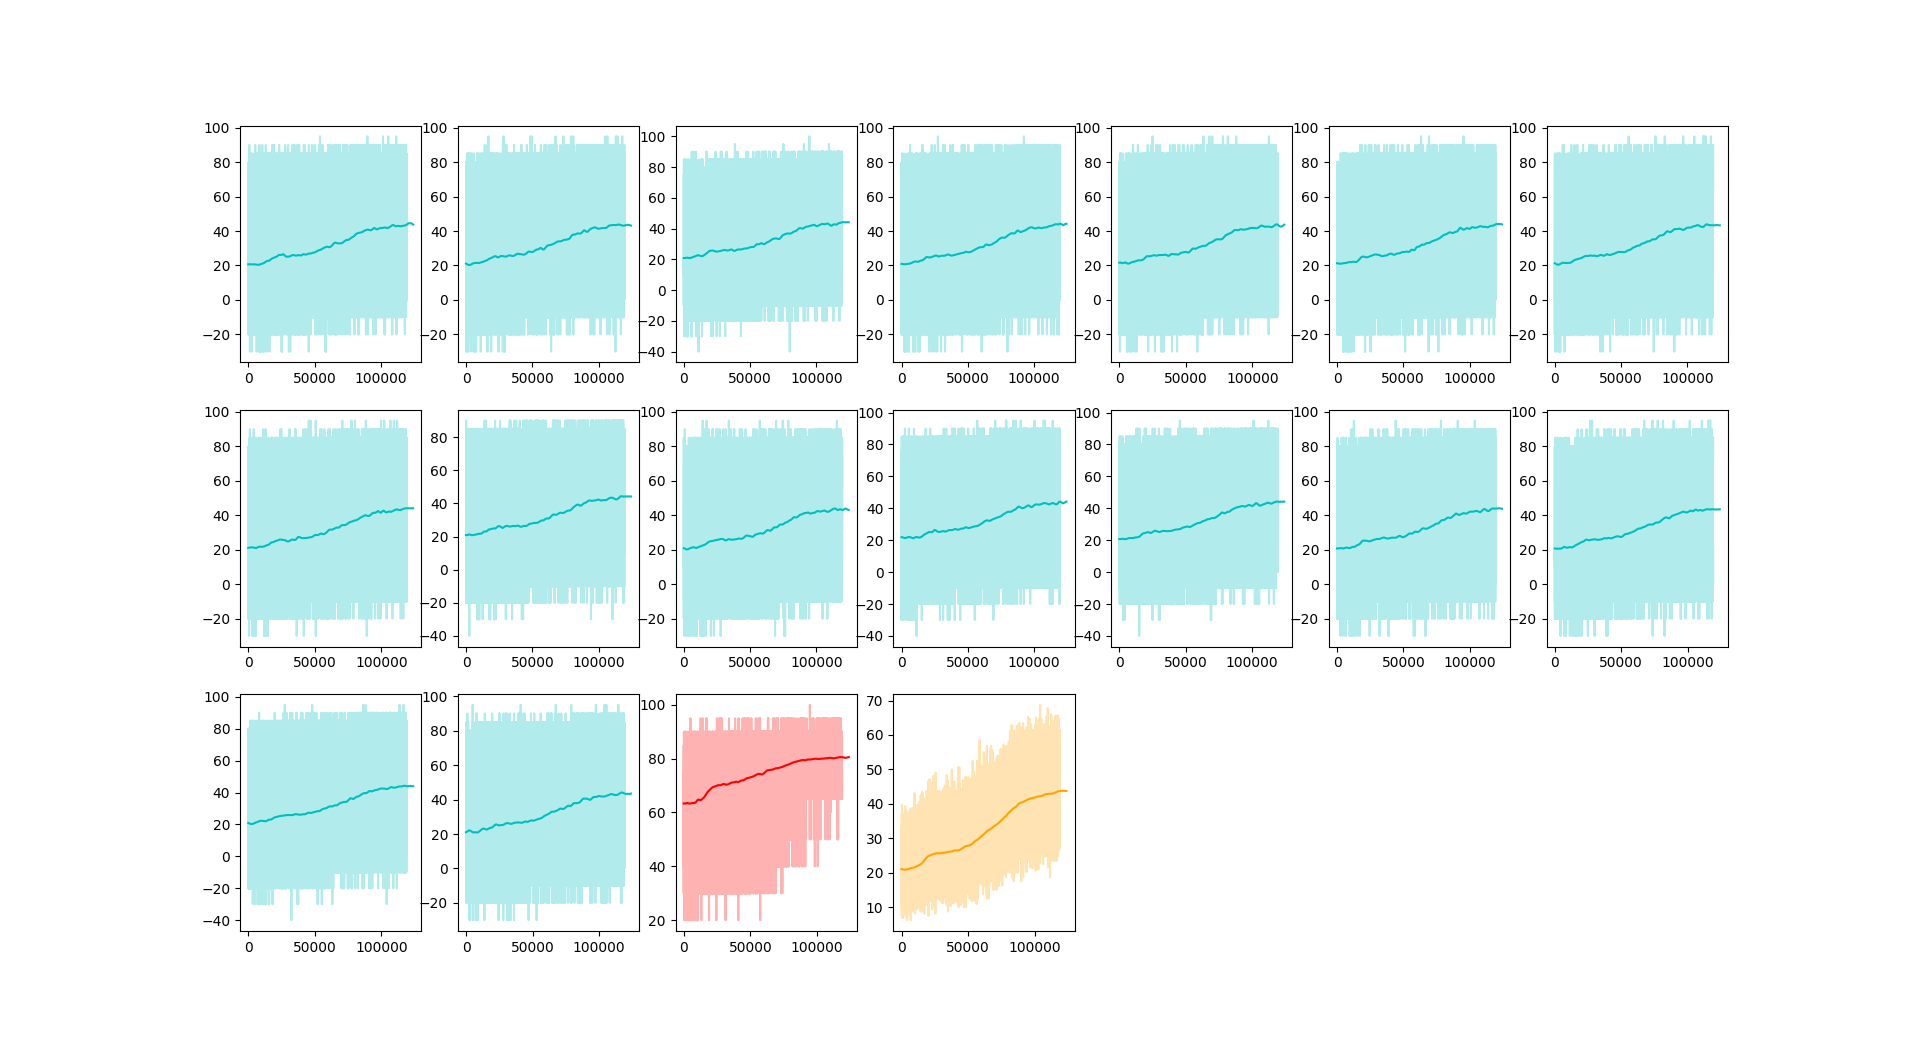
\includegraphics[width=1\textwidth]{Figures/plot_example_preview.png}
  \caption{Example output of the \lstinline{plot_baselines} module. Output was generated from 16 environments(blue) and also contains a plot maximizing rewards over all environments(red) and a plot measuring the mean over all environments(orange) }
	\label{fig:plot_example}
\end{figure}

Figure \ref{fig:plot_example} shows an example output of this module. Generated are plots for each individual environment/log file of a run in blue. From the data for these plots two additional plots are created: one plot representing the mean reward over all environments for each episode, and one plot representing the maximum reward that was achieved across all environments for each episode. Each sub plot contains both the actually achieved or calculated values in the background with low opacity, and a smoothed version of the graph, which is calculated using numpy's convolve function and a window of a few thousand values. This smoothed graph gives a rough trend curve, making it easier to discern how much reward was achieved on average over a certain period of time. 

Averaging twice, once across environments and once across timesteps might make results seem worse than they actually are however, because this really emphasises consistency of results more so than actually getting the highest possible rewards. This is the reason that in addition to the graph of mean rewards the graph of maximum values is shown as well. As Figure \ref{fig:plot_example} shows, the rewards achieved by the individual environments tend to be substantially similar, which is somewhat expected, because their decisions come from the same neural network. For this reason only the max and mean plots are shown as evaluations in the Evaluation chapter and not individual environment results. 

\subsection{Environment Wrappers}
\label{sec:wrappers}
The environment wrappers are a very important component of this project. They are also not only useful in this project, but instead are designed to be used independently as well. These wrappers fulfill two primary functions. Firstly they provide a unified and familiar interface to the actual game environment. The interface is modelled after and actually extends the OpenAI Gym Environment base class. This approach was chosen, because the OpenAI gyms are the industry standard for reinforcement learning environments and should be well known to anybody working with RL algorithms. Even many environments that are not OpenAi gyms follow a very similar pattern.\\
The pysc2 environment however has a number of key differences which make it a little bit more difficult to adapt different RL algorithms for it. Using these wrappers however it becomes straightforward to apply, for example, the OpenAI Baselines algorithms to StarCraft II scenarios as was done in this project. The adaptation of other algorithms to PySc2 should be simpler with these wrappers also.

The second function of these wrappers is to add an additional layer of control over the environment.
Instead of exposing the full complexity of the PySc2 environment, with millions of possible actions and a multitude of feature layers and discrete features, utilizing these wrappers one can choose exactly which features to expose and which actions to allow. This permits more precise tuning of the difficulty of the scenarios. \\
In the case of the simplified variants of the scenarios these wrappers do not even expose the standard PySc2 actions at all and instead follow somewhat of a hybrid approach, mixing conventional programming with reinforcement learning. In these environments a number of high level and more abstract actions were implemented that are more or less specific for one scenario and only these high level actions can then be used by the reinforcement learning algorithms.

The actual implementation of these environment wrappers and how they integrate into the rest of the system has undergone many changes and overhauls over the course of this thesis, as they are binding everything together making them especially important for this project.
In the beginning the goal was to keep the wrappers as general-purpose as possible, with each wrapper working for as many different scenarios as possible. However, the way the scenarios developed and especially how restricted they are regarding their input layers and available actions this turned out to not be appropriate. In contrast the current implementation requires one environment specifically for each map, but in return the individual wrappers have become much simpler and smaller.

All environments extend the Base Environment class BaseEnv, that now contains most of the functionality needed by the wrappers.
The BaseEnv wrapper extends the OpenAi Gym class and therefore needs to implement the methods

\begin{itemize}
\item \lstinline{_step()}
\item \lstinline{_reset()}
\item \lstinline{render()}
\end{itemize}
and also the properties of
\begin{itemize}
\item \lstinline{action_space}
\item \lstinline{observation_space}
\end{itemize}

The \lstinline{render} method can be simply left empty though, as PySc2 handles it's own rendering and does not require a stepwise rendering call. The \lstinline{_step()} method needs to advance the environment taking the action specified by the action parameter and returns the tuple: \lstinline{(s_, r, done, info)}, where

\begin{itemize}
\item \lstinline{s_} is the new state of the environment, after the taking the action a
\item \lstinline{r} is the new reward
\item \lstinline{done} is a boolean, representing whether the current episode is over
\item \lstinline{info} is an arbitrary python dictionary, that may contain information not directly impacting the environment
\end{itemize}

This \lstinline{_step} function is the same for all wrappers and is not individually implemented.

The actual environment step is done by the PySc2 environment which requires a PySC2 FunctionCall object. However, this step function returns a complex timestep object, that is not usable in this state. Before this state can be used by a reinforcement learning algorithm it still needs to be transformed, which is done by the instance method \lstinline{get_state}, which in turn uses the static \lstinline{get_input_layers} method of the helpers module. The \lstinline{get_input_layers} method goes through all available screen input layers of the current state(minimap layers were largely ignored in this project, as the scenarios only use one screen) and reshapes and concatenates all layers found in the private \lstinline{_input_layers} variable, that has to be set by each wrapper individually and only contains dummy data for the base environment. This approach of representing the state was chosen in order to be able to restrict the observations for each scenario to only exactly the information that is needed to solve it. The other option would have been to always concatenate all layers for every scenario. Unfortunately this would leave a lot of irrelevant information for each specific scenario, complicating and slowing down the learning process.

The \lstinline{_reset} method simply calls the reset method of the PySc2 environment and afterwards returns the state again using the \lstinline{get_state} method. While this is all that is necessary for \lstinline{_reset} to work it may be advisable to completely rebuild the environment every approximately 8000 Episodes depending on the complexity of the map. This is because memory usage of the StarCraft II engine increases considerably the longer a map is running. Likely this is because StarCraft II needs to keep a record of all actions and unit information since map start in order to reconstruct and save replays of the map. Rebuilding the environment is done by deleting the \lstinline{_env} variable and setting it to a newly created environment. Although PySC2 already automatically reloads the map after a maximum amount of steps memory problems can manifest even before that, which is why such a rebuild is implemented here aswell.

The \lstinline{action_space} and \lstinline{observation_space} properties return a gym.spaces.discrete value and gym.spaces.Box respectively. These gym types are used instead of returning an integer and a numpy shape tuple, as they offer additional functionality and a different interface, that are used by OpenAI Baselines algorithms.

In addition to these methods and properties required to extend the gym environment class there is one more method that all environment wrappers need to implement individually, the \lstinline{get_sc2_action} method. This method gets the action chosen by the neural network as a parameter and has returns a PySc2 FunctionCall object that represents the actual StarCraft II action that the agent will take. This is implemented on a per wrapper basis, because this lets the wrappers handle the same actions slightly differently if need be.

To properly extend the BasEnv class only three things need to be implemented.
The first is a list of available actions ids. The ids should be the same used in \\pysc2.actions.FUNCTIONS. 
In simplified variants of scenarios
Action ids may be duplicated in this list, as each action in this case is attached to one of the directions up, down, left or right but still refers to the same underlying PySC2 function, only with other parameters attached.

The second one is a list of input layers, the combination of which should represent the state of the environment. The layers should be specified by ids set in pysc2.features.SCREEN\_FEATURES.
This is very similar to \lstinline{_actions}

Lastly the \lstinline{get_sc2_action} method has to be implemented.
For the simplified environment versions this method makes use of the current state observation and the \lstinline{get_shifted_position} method of the helper module for determining the next location to move to or attack towards. It then returns a PySC2 FunctionCall object that can be used, to take a step in the PySC2 environment. The type of action is chosen according to the index provided by the \lstinline{action} parameter in the \lstinline{_actions} list.

One unique environment is the sim\_proc\_env or Simulated Process Environment. It is not in fact a wrapper for a specific map or scenario and instead is an optional wrapper for all other environment wrappers. This additional wrapper is needed for validation and rendering purposes regarding the OpenAI baselines algorithms. It uses the same interface as and therefore "simulates" the SubprocVecEnv that is normally used when running the baselines algorithms. The SubprocVecEnv is a multiprocessing environment built for running multiple environments in parallel. When debugging, rendering, and validating this environment is problematic, which is why it is substituted by the sim\_proc\_env. Running the baselines algorithms on the other environment wrappers directly is not possible, as the algorithms do batch processing and expect to interface with multiple environments at all times.

Apart from the actual environment wrappers each StarCraft II map also needs to get attached to an object that extends pysc2.lib.Map, as these Maps objects is how PySC2 loads the .sc2map file into the game client. These objects include some parameters that can also be set globally for PySC2 but most importantly the filename and location of the map. The load\_scenarios function of the maps.scenarios module creates global Map types according to an array of Mapnames.

\subsection{Helper Module}
The helper module contains static functions that are useful globally in this project and do not really fit into a specific class.

One of the most important functions is the \lstinline{get_env_wrapper} function. \lstinline{get_env_wrapper} is called every time a pysc2 environment needs to be build, whether during initialization or when rebuilding an environment, and returns the correct wrapper for the map specified by the commandline parameter.
In order for this to work a naming convention has to be adhered to: map files in the \lstinline{StarCraftII\Maps} directory and the wrapper class have the same name and are written in upper camel case, while the module containing the wrapper class located in the \lstinline{util.environments} module is written in snake case. The function first imports the necessary module and class and then returns the object created by the class's constructor.

Also used for all scenarios is the \lstinline{get_input_layers} function. This function is used by all wrappers in their respective \lstinline{get_state} methods and by extension \lstinline{observation_space} properties. It requires the current pysc2 timestep and a list of layer ids, that should be part of the observation/state of the environment. The method creates the state, that is sent to the neural network by extracting the specified layers from the PySC2 timestep object and concatenating them into one 3 dimensional matrix. Each layer basically functions as one channel in a 2D image that is processed by the Convolutional Network.  

In addition to these functions, that are used in all scnearios, the helpers module contains a few functions only utilized by some environments.
One example is the \lstinline{get_shifted_position} function. It takes the current pysc2 timestep, a direction and a distance in map units as parameters and returns screen coordinates, that are the result of shifting the current position of friendly units in a certain direction by the specified distance. This is used for all of the simplified variants of the environment wrappers, where for example Move Screen or Attack Screen commands are converted into grid movement.

\section{A3C Algorithm}
\label{sec:ac3impl}
\subsection{Architecture}
The implementation of the A3C algorithm used in this project is adapted from the implementation at \citep{a3ccartpole}.
This implementation is somewhat different from the one proposed in the original paper. In fact, it is closer to the GA3C implementation \citep{DBLP:journals/corr/BabaeizadehFTCK16}, and depending on which parallel processing architecture is chosen even to A2C.
\newpage
This A3C implementation features five components/classes:
\begin{itemize}
\item a3c - class for initialization and running of the algorithm
\item Brain - class holding the global neural network model and graph
\item Agent - class choosing actions and putting samples into the training queue
\item Environment - class handling the RL environment
\item Optimizer - class transferring data from the queue to the GPU and training the network
\end{itemize}
that are described in more detail in the following sections.
The biggest difference to the standard implementation of A3C is that instead of having individual network parameters for each worker thread, there is only one global neural network with one set of parameters. This architecture is depicted in Figure \ref{fig:a3c_over}. 

 \begin{figure}[htb]
  \centering
      \includegraphics[width=1\textwidth]{Figures/A3C_Project_Overview.pdf}
  \caption{ Overview of the A3C Architecture used in this Project. Shows the interaction between the different high level component classes of Environment, Optimizer and Brain}
 \label{fig:a3c_over}
\end{figure}

The advantage of this version of the A3C algorithm is that it manages to utilize the GPU more effectively, by using multiple optimizer threads that only have the job of feeding samples to the GPU. One disadvantage is that for performance reasons this architecture requires a relatively large batch size, meaning that training samples are not processed immediately. This introduces considerable policy lag, where the network chooses actions always slightly behind the current policy as given by the available training samples. Also, special neural network layers like LSTM, that process a chain of samples in order to process time series do not work any more, as samples are put into the network by all agents completely asynchronously abstracting from all temporal information that connects the samples.

\subsection{A3c.py}
The A3c module is what is started by the train module and initializes all other objects and modules required for running the A3C algorithm. It also oversees the starting and stopping of the parallel processing environment. The A3C class features only it's constructor and a run function as methods, as is required by the train.py module.
The constructor creates all the environments and optimizers, the global neural network in the form of the Brain class and the gamma parameter used in the n step return.

Environments and Optimizers are only created here when the validation flag is not set, as during validation no optimizers are needed, and a single validation environment is created elsewhere.
The \lstinline{none_state} created in the constructor is an empty placeholder state that will later be used during the optimization step.

The run method starts all threads, and then sleeps until the time specified by the \lstinline{run_time} Flag is over, with occasional breaks for logging and saving intermediate models, and then stops and joins all threads.
For a validation run the code is somewhat similar, but it uses only one environment, no optimizers and no logging.

\subsection{Brain}
\label{sec:brain}
The Brain contains the neural network code and represents the global network used by all environments and agents. During initialization a new Keras Model and tensorflow graph are created. The Keras model uses the functional approach to model creation in order to make use of multiple in- and outputs. More information about the actual neural network can be found in section \ref{sec:polmodel}. 

The method creating the tensorflow graph definition starts off with defining placeholders for the inputs and outputs of the neural network and loss functions. It then gets \lstinline{p} and \lstinline{v} values from the model using the State placeholder \lstinline{s_t}, \lstinline{p} being the softmax activated action array and \lstinline{v} being the value function result for this state.

Next, the loss function is constructed. As described in section \ref{sec:a3ctheory} it has three distinct components: the policy loss, the value loss and the entropy, that can each be weighted in order to put stronger or weaker emphasis on these components. RMSProp has been chosen as an optimizer here as well.

After that follows the set of functions that are exposed to environments, agents and optimizers for the use of this "Brain". First are the predict functions used to choose actions and/or query the current estimate of the value function.
Using tensorflow's default graph they simply call the predict function of the keras model and return the variables that are needed.

Also, the brain offers the optimize method, used by the optimizer threads in order to train the neural network. This is done in batches. To that effect, the size of the training sample queue is checked and if it is smaller than the batch size the thread simply yields. Otherwise the queue is emptied and transformed into vertically stacked numpy arrays or vectors, each containing all values for one of the elements in the tuple $(s,a,r,s\_,s\_mask)$. 

The rewards up until this point have been only the immediate discounted rewards of
$$r = r_0 + \gamma r_1 + \gamma^2 r_2 + ... + \gamma^{n-1}r_n$$
without the estimated value of the state afterwards $\gamma^nv(s_n)$. This component is added here by querying the keras model for the current value function estimation.

In order to do this efficiently through the use of matrix multiplication the $s\_mask$ vector is needed. It is a mask containing information on whether the states were terminal, or not. If a state is terminal the value function component of the discounted reward should not be added, which can be achieved by simply multiplying the predicted value function with the mask vector.
\begin{lstlisting}[language=Python]
r = r + shared.gamma_n * v * s_mask
\end{lstlisting}

After computing the rewards the network's optimizer's minimize function is run, with these vectors fed to the network using a feed dictionary.

\subsection{Environment}
The environment class extends the threading class, contains an agent and an environment wrapper and is responsible for running the training episodes. It does this continuously after calling it's run method until a stop signal is sent.

Each episode starts by resetting the PySC2 environment through it's wrapper, after which it runs indefinitely until either the environment returns information that the episode is over, or the thread is stopped. In each step of an episode the environment is yielding for a short duration specified by the \lstinline{thread_delay} flag. While this is not always used, this enables the possibility of efficiently using more environments and optimizers than CPU threads are available.

After that, an action is chosen by the agent and then this action is used to perform the next step in the environment. If the episode is over, the successor state \lstinline{s_} is set to None, after which the agent initiates training of the neural network with the use of the current state \lstinline{s}, the chosen action {a}, the current reward \lstinline{r} and the next state \lstinline{s_}. Lastly, the current state is set to the successor state and the next step begins.

\subsection{Agent}
The agent class is responsible for choosing actions as well as keeping a sample memory in order to calculate an n-step-return reward. As it's parallelism is already granted by being created inside the environment class, the agent does not need to be a separate thread.  

Upon calling the act method an action is chosen according to the current state $s$.
To achieve this, the neural network first predicts action probabilities according to the state. Afterwards one of these actions is chosen at random with respect to the probability vector returned by the neural network. A different approach could be to always choose the most probable action through
\lstinline{a = np.argmax(p)}. While this would be useful for a perfectly trained neural network this would largely prevent exploration. If the network only chooses the actions it deems best, it is completely closed off to state spaces that lie outside of it's current view and which might be much better. Without such exploration the network is almost sure to converge on a very suboptimal local maximum.

The original code this A3C implementation is adapted from implemented an additional method of exploration, $\epsilon$-greedy. With $\epsilon$-greedy, $\epsilon$ percentage of actions were chosen completely at random not taking into account the neural networks' predictions at all. The value of epsilon was then linearly decayed over the course of training. This was removed in this project however, as having two different methods of exploration active at the same time did not seem to provide any benefit.

The train method both adds the training samples produced by the agent in conjunction with the environment to the memory array used to calculate the n-step-return rewards and removes samples from the memory in order to add them to the actual training queue, that is transferred to the neural network by the way of the optimize method described in section \ref{sec:brain}. All samples are stored in the memory, but not every call of the train method also adds a sample to the network's training queue. Samples are only added to the queue if either more than n samples are in memory, with n being the size of the n-step return, in which case only the earliest memory sample is added, or if an episode is finished, in which case the entire memory is dumped into the training queue.

The n-step return is not calculated individually for each sample, but instead kept as a property of the agent and is calculated in a rolling manner, with each new sample adjusting the reward. At the end of each episode this rolling reward is reset. 

\subsection{Optimizer}
The optimizer class extends the threading class as well and is the simplest of all the classes with less than 20 lines of code. After initiating its run method it simply repeatedly calls the optimize method of the Brain object, until a stop signal is received.

\section{OpenAI Baselines}
\label{sec:baselinesproj}
\begin{figure}[htb]
  \centering
      \includegraphics[width=0.7\textwidth]{Figures/Baselines_Overview.pdf}
  \caption{ Overview of the OpenAI Baselines Architecture and how it integrates into this project. While high level control of the algorithm and its Network Policy in addition to the environment wrappers reside inside this project, they interact with the Runner, Model and parallel processing environment from inside the OpenAI Baselines module.}
  \label{fig:openoverview}
\end{figure}

While the environment wrappers do most of the work to integrate the OpenAI Baselines algorithms into this project some modifications were made to the actual baselines algorithms. As each baselines algorithm has to be adapted individually this project focused specifically on the A2C and ACKTR algorithms.

At first the modifications were done on a copy of the entire baselines module, that was integrated into the projects git repository entirely. The current state is however, that only the few necessarily modified files are part of the project and the baselines module still has to be installed separately. This architecture is illustrated by Figure \ref{fig:openoverview}. There are three major components that had to be modified.

The first component are the run scripts contained in the individual run\_atari.py files. These were built into a class that also contains the \lstinline{learn} function of acktr\_disc.py and a2c.py. With their modifications they fulfill roughly the same role of initiating and running the high level operations of their algorithms, as the ac3.py does for the A3C algorithm.

The second component is the policy model. Even though it is fully written in tensorflow and not keras, the abstract utility functions offered by the baselines project made it easy to reconstruct the same model that is used for A3C.

The last modification was to finish the implementation of features to load and validate a previously trained model. While there were already save and load functions attached to the model they were not used in the code. Also there was no option to run only a single, non sub\_proc environment, which is very useful for validation purposes. 
Lastly the actual training of the model was disabled if the validation Flag was set in order to not skew results.
For rendering purposes during validation an additional per step delay was added as well, as to limit execution to only a few steps per second, making it easier to watch for humans.

\section{Policy Model}
\label{sec:polmodel}
While quite a few configurations of CNN's were tried over the course of this project the main one in use for many of the evaluations is the structure proposed by DeepMind in their Atari-Net and that is also mentioned in \citep{sc2}.

It features two convolutional layers with a RelU activation function and no pooling layer in between.
The input size of the first convolution layer is directly determined by the \lstinline{observation_space} property of the respective environment wrappers.
Using pooling layers for these scenarios specifically is not necessary, and might even be a hindrance since the translation invariance that it brings with it does not translate well into the game world where the specific coordinates might matter a great deal. When learning scenarios that utilize a bigger game world of more than one screen, like for example the competitive Player vs Player maps this translation invariance will likely become much more useful.

Following after the convolution steps is one fully connected layer, which then feeds the outputs for the action and the value function. This configuration has been working very well for all scenarios with one small caveat. If there is single single Zergling on the Map the network has much more difficulty determining its position than with groups of Zerglings or other units. The Zergling is the smallest unit in the game of StarCraft II with the next biggest units being twice its size, and is also a unit that is rarely on its own, meaning that this is a very rare and isolated problem.




\section{Extensions to the RL Implementation}
\label{sec:extensions}
In order to help the reinforcement learning algorithms to perform optimally in the StarCraft II environment some extensions were made to the core algorithms, which are described in the following subsections. Section \ref{sec:multistate} covers how the environment observations are formed and can be used as the networks input, with the addition of a state history, recording the latest time steps. Section \ref{sec:spatial} will then discuss options for modelling the vast action space of StarCraft II efficiently and lastly \ref{sec:replearn} will describe an attempt to make use of StarCraft II replays as training experiences and building a semi-supervised version of A3C.

\subsection{Multi Input States}
\label{sec:multistate}
One important aspect of reinforcement learning is defining what information each state $s$ contains and how it is presented to the reinforcement learning algorithm.
In the PySC2 environment this decision lies primarily with the choosing of screen and minimap input layers.
Each of those layers represents a single channel image with the dimensions $(X, X, 1)$ with $X$ being either the screen resolution or the minimap resolution parameter set during start-up. Non quadratic screen aspect ratios are not permitted by PySC2 as of now. As having differing screen and minimap resolutions is very reasonable, two input layers are needed for the neural network model. Alternatively, padding on the smaller of the two can be used to equalize their size.

Multiple input layers can then be combined by treating the state of the game as a multi-channel image, with dimensions $(X,X,Z)$ where X is the image resolution and Z is the number of input layers representing the state $s$. Each layer is then one channel of the input image.

Not all game information is found in those input layers however. The vector of discrete information available in PySC2, for example, needs to be an extra model input as well. This input should not lead into the convolution steps of the model though, and should instead directly connect into the Fully Connected layers, effectively merging with the flattened convolution outputs.

The last extension regarding the state of the environment would be to include a history of timesteps to incorporate temporal information into the state. 
Using a history of timesteps to define the state of the Environment, as was successful for example while learning the Atari games \citep{DBLP:journals/nature/MnihKSRVBGRFOPB15}, can not only improve training results in general, by giving the algorithm a backwards view on what it had previously done, but can also be strictly necessery in the case of MDPs with limited information. The state for a game of StarCraft II for example can not be fully described by the current state, mainly because the fog of war obscures most of the map and the player has to extrapolate what the opponent could be doing from previously gained information, but also because the direction and speed of moving units can not be determined by a single time slice. While this is not necessary for the specific scenarios that were tested in this project, it should still be somwhat of an improvement.

The implementation for this is very straightforward. In order to use this history across all environments it is implemented within the base environment \lstinline{base_env} class. The history is stored as a simple array with the length of the specified history size parameter. It is initialised and reinitialised at the start of each episode in a way that each element of the array is the first state of the episode. This is done to keep the dimensions of the state the same, although in the first few states no full history is available yet. A different option would be to fill it with empty states instead, but there should be negligible difference. In each subsequent step, a new step is added to this history, and the oldest timestep is removed. 

The only other modification that had to be made was to the \lstinline{get_state} method of the same class and the corresponding \lstinline{get_input_layers} method of the helpers module. The \lstinline{get_input_layers} module now has the entire history as a parameter instead of the current timestep and concatenates all layers accordingly. As the \lstinline{get_state} method is also used to calculate and expose the \lstinline{observation_space} property, which is used to determine the input dimensions for the Neural Networks both in the OpenAI baselines and in the A3C algorithms, no further code modifications were necesssary.  

The biggest disadvantage to using this history size is that it slows down training speed dramatically. Using 4 timesteps for example the steps that can be gone through per second is almost halved. For this reason one has to carefully weigh the improvements that this feature brings with it against the slower training speeds. 

One additional slight disadvantage is a higher memory consumption. Since much of the memory usage of this program is tied up in the environment state, especially in regards to the training queue for the A3C algorithm, increasing the size of a single state results in an increase of the programs memory with almost the same factor. with history sizes above 5 this can lead to memory shortages very quickly and makes it a requirement to utilize more optimizers and smaller batch sizes, that keep the training queue as small as possible. This is true in particular, because the optimization itself is slower, as more data has to be transferred to and be processed by the GPU. As training samples are directly processed in a step wise fashion by the OpenAI Baselines algorithms this is less of an issue for them. 

Instead of using Keras' Conv2D layers for representing the environment with concatenated history timesteps, there is also another option available: In addition to the 2D Convolution Layer Conv2D Keras also offers a 3D Convolution Layer Conv3D. Using that, the state $s$ could be represented with dimensions $(X, X, Z, T)$
With T being the number timesteps including the current one, that should be part of state $s$. This was not tested however.

\subsection{Spatial Information Policies}
\label{sec:spatial}
So far only the implementation of high level actions, that do not reflect actual StarCraft II or PySC2 actions were discussed. This section discusses multiple options for letting the policy model handle PySC2 actions directly. One unique problem of the StarCraft II environment is, that in every step there are many complex actions available, which is caused by many actions requiring spatial information in the form of screen or minimap coordinates.

The naive approach would be to simply flatten all action and parameter combinations into one action list and treat them as any other reinforcement learning problem. This is not very feasible however, as this can easily result in hundreds of millions of actions depending on the screen and minimap resolutions. For the default resolutions of 84 for screen and 64 for minimap for example there exist 101938719 Unique actions.

DeepMind's paper \citep{DBLP:journals/corr/dmsc2} proposes two better approaches one of which was implemented in this project. Both of them are depicted in Figure \ref{fig:pysc2_state}.
The approach not implemented here is to use a Fully Convolutional Policy, as used in DeepMind's FullyConv neural net. In contrast to a regular CNN Policy the FullyConv net does not discard the spatial information gained during the convolution steps by adding flattening and fully connected layers. Instead, the convolutions are carried till the end with stepwise padding in order to maintain the input resolution. In the end this spatial information is directly carried over into the spatial actions.

The last approach is to separate the spatial parameters from the actions themselves and let the neural network learn them independently. This means, that the model now has two additional outputs for the potential x and y coordinate of an action. For actions that do not require spatial information these outputs are simply ignored. Of course this separation does not inherently reduce the complexity of the problem, as multiplying the number of actions with the possible x and y coordinates still results in the same number of possible actions. The advantage is however, that the correlation of values is clearer in this approach. 

\begin{figure}[htb]
  \centering
      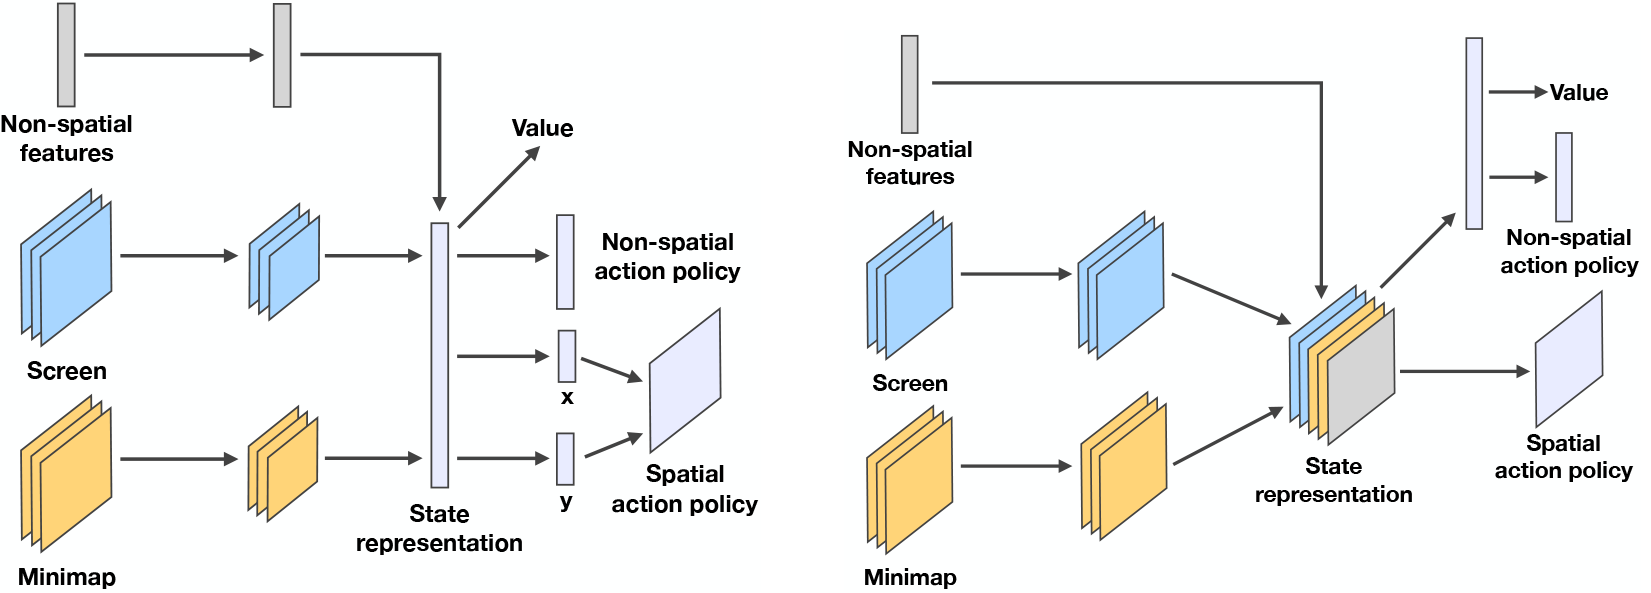
\includegraphics[width=1\textwidth]{Figures/sc2le/sc2le_state.png}
  \caption{The Policy model for separation of spatial action parameters from the actions themselves(Left) and the policy model for the fully convolutional approach(Right). Both approaches use a CNN to process the minimap and screen features, but while the state is flattened for the first approach, the state and resulting actions stay convolutional for the entire procedure for the second approach \citep{DBLP:journals/corr/dmsc2} }
  \label{fig:pysc2_state}
\end{figure}


In order to implement this method of incorporating additional action information into the policy considerable modifications have to be made both to the A3C implementation, and the OpenAI Baselines algorithms. For the OpenAI Baselines algorithms this was done mostly in the python modules already adapted for this project residing in the \lstinline{baselines_mod} module. The first modification to be made is to the neural network policy, adding two additional outputs. Both of these connect to the same fully connected layer as the value function and action outputs and also use softmax activation. Only the CNN policy was modified, as other available policies for acktr and a2c were not tested in this project.

The other difference is in the loss function, which now incorporates not only the action loss but also the parameter loss. For the A3c algorithm both the policy loss and the entropy is modified, with the new policy loss being:
$$J(\pi) = -A(s, a) * (\alpha * log P(a) + \beta * log P(x) + \delta * log P(y)$$
with $\alpha$, $\beta$ and $\gamma$ being three new hyperparameters, that determine the importance of choosing the correct action versus choosing the correct parameters. For simplicities sake these were not accurately tuned over the course of this project and instead set to 1, 0.5 and 0.5 respectively. These values were chosen. because choosing the correct action was deemed considerably more important in the specific scenarios of this project, and there should be made no difference between the importance of x and y parameters.

\subsection{Learning from Replays}
\label{sec:replearn}
One of the challenges with very complex environments like StarCraft II with incredibly huge state spaces and accordingly manifold state transitions is that it can be difficult for an environment to even encounter advantageous states in order to learn from them. This is exacerbated by the fact, that episodes in the StarCraft II consist of hundreds of steps even in small mini-games and tens or hundreds of thousands of steps in the actual game where very precise action is required to gain any reward at all and tangible rewards can lie hundreds of steps in the future. 

One attempt to deal with that challenge that was made in this project is to use pre-recorded replays in order to augment the training samples that are generated by the environment. This is done in a similar manner as experience replay was used to augment training of, for example, the DQN algorithm \citep{DBLP:journals/corr/abs-1712-01275}.
Instead of replaying experiences that the agents have already encountered however, human replay samples can be used for augmentation. Still, the training experiences of the human players are viewed and processed from a first person view, which means that the experiences represent exactly the features and actions the algorithm could and would see. 
This is in contrast to learning from a third person view, which would also be a possibility using the PySC2 framework and is a research topic discussed for example in \citep{DBLP:journals/corr/StadieAS17}. 

For the scenarios utilized in this project third person imitation learning would not be very useful, as all players and also third party spectators have roughly the same view on the environment. Nevertheless, for learning the entire game of StarCraft II this is a technology that could prove very useful. In a competitive 1v1 game the agent could learn from both players at the same time, by posing as the third person spectator with the full view of the entire game, instead of just learning from the actions of a single player in first person view.

This introduction of pre-existing data into the reinforcement learning process most closely relates to the research topic of semi-supervised learning, e.g. \citep{DBLP:journals/corr/FinnYFAL16}, \citep{DBLP:journals/corr/schgan}. It is not entirely the same however. Semi-supervised learning mostly concerns itself with incorporating a gold standard, i.e. labelled training data. This does not apply to what was tried in this project, but some of the same concepts apply.   

Learning from human replays has the advantage, that the policy can be improved by being shown very specific state spaces which are desirable. The challenge for the algorithm then somewhat shifts from searching for states which give maximum reward to searching for a set of state transitions, which lead to such a state that is already known. There are possible disadvantages to this approach as well, though. Adding too many human training samples or samples without enough variety for example could potentially discourage exploration and lead to over-fitting of the neural network weights, which could result in the algorithm converging on suboptimal local maxima. Additionally exposing the algorithm to the human strategy of solving a scenario might prevent it from finding it's own different and possibly better overall strategy. For this reason, this augmentation process should only really be used if one can be sure, that the recorded replays contain the most optimal way of solving a scenario.

The replays that were used for this augmentation were recorded by playing the scenario maps over and over from within StarCraft II. StarCraft II has the built in feature of saving games as .SC2Replay files which is taken advantage of here. These .SC2Replay files contain all necessary map information, all actions that were executed by all players and their results. This information can then be used by the SC2 Engine to reconstruct the game and review it in its entirety. Nevertheless, the way this information is stored is not very useful for usage in an RL algorithms. Therefore the first task is to convert this .SC2Replay data into a more convenient format.

This adds a new third entry point to this project, the convert\_replays module. The main objective of this module is to take all replays available for one specific scenario and output one easily readable file that can be plugged into the already existing algorithms as seamlessly as possible.
In order to achieve this, this module employs the replay playing functionalities provided by the PySC2 framework. Stepping through a replay in PySC2 is considerably similar to stepping through an active PySC2 Environment, but there are some key differences.

In order to get training samples that fit the experiences of the RL algorithms best, the same step multiplier of 8 game steps for each 1 environment step is used again here for replays. Similarly the same resolution for the rendering of input layers has to be used. During each step one observation/state is obtained from the SC2 engine, not by submitting an action like it would be with an active environment, but by simply querying the replay controller. Unfortunately this observation differs greatly from the observations obtained from an active environment and is in many areas even incomplete which is one of the difficulties that were encountered trying to implement this approach. The information that needs to be extracted in each step is essentially the same tuple of 
$(s, a, r, s\_)$
that is used in training. As this replay conversion is only implemented for versions of the algorithms that employ spatial information policies using screen coordinates, x and y coordinates for the action have to be retrieved as well. The choice to exclude the simplified version of the scenarios and with that the standard action list based versions of the algorithms was made because for one it is somewhat difficult to create human replays with their restrictive movement patterns and also it is not always possible to recreate the necessary abstract actions from an arbitrary replay.

The most straightforward information to retrieve is the action that player 1, the human player made. The actions property of the observation contains a list of all actions that were made since the last controller step. As the AI for scenarios is controlled strictly from within the map editor, this list only contains the human players actions. Additionally the human players creating the replays should restrict themselves to not act faster than the step multiplier chosen implies, which for a multiplier of 8 is 3 actions per second. This results in the actions property having either 0 actions in which case the current step is simply ignored or 1 action, which is then used for the training sample. As the algorithms do not learn on PySC2 action ids directly however, and instead on the ids provided by the respective environment wrappers, the wrappers' \lstinline{_actions} array needs to be queried for the index of the PySC2 action. In order to get the correct wrapper this means, that the module needs the map of the replay as a parameter. The x and y coordinates can also directly be obtained from the action object.

Next, the observation state is obtained. The input layers are stored somewhat similarly to an active environment but instead of numpy arrays they are stored as a byte buffer, with each pixel either being represented as a boolean, a char, or an integer, depending on the maximum value of the layer. For all byte sized layers numpy's \lstinline{frombuffer} method is used for conversion. Unfortunately, layers like the creep layer used in the Find Ultralisk With Creep scenario that contain only bit information are not stored in a way easily read by numpy. Instead of the byte sized booleans used in numpy they are stored as a bit array but still using the datatype bytes. For this conversion a custom function was implemented, that first converts the bytes into an array of unsigned integer bits and then converts each group of bits into it's actual integer representation. \\
The \lstinline{input_layers} property of the environment wrapper is used in order to determine which layers should be used, and to reproduce exactly the same state the wrapper would see if it was an active environment.

The reward can be obtained directly through the curriculum score property of the observation. The problem with using this score as a direct reward however would be, that the algorithms, both A3C and ACKTR/A2C, do not use direct rewards for training and instead use discounted rewards making use of an n-step-return. As the samples generated by this module are supposed to be independent from each other this calculation can not be done on the fly during training and is therefore calculated here. This n step return is calculated by using a standalone agent object from the A3C Algorithm. This Agent is not attached to an environment or a brain and is directly fed the replay samples, which it calculates the discounted rewards for and then puts the completed samples into the queue, similar to how it would do it during A3C training. Of course the rewards calculated in this way are only really usable in the A3C algorithm, and even then only if the same values for the gamma parameter and length of n-step-return are chosen during training. 

The OpenAI Baselines algorithms employ a slightly different strategy for their n-step-return, that is considerably harder to replicate. The main difficulty lies in the way, that that the baselines algorithms use the current value function as given by the neural network in their calculations for their discounted rewards. As the learning from replays feature was implemented very late into this thesis, there was not enough time to adapt it for the Baselines algorithms as well and therefore this functionality is currently only available for the A3C algorithm.

In order to calculate this discounted reward the agent needs one more piece of information: where the end of each episode is. Unfortunately, this information is not easy to obtain due to bugs or missing features in the StarCraft II Machine Learning Protocol. There are four main ways that should be able to detect whether an episode is over due to how they are built in the map editor:

\begin{itemize}
\item player\_result - The player result property should be filled, each time the main objective of a map is set to completed. While this is correctly detected while playing within pysc2, during replay view this property gets only filled at the end of the replay with a generic win or loss information
\item chat message - in order to reset the episode the framework writes "reset" into the chat. While there is a chat log property on the replay observation it stays empty no matter what is written in chat.
\item episode timer - if an episode is over the episode timer is either completed or paused. the replay observation does not contain timer information however.
\item UI - When an episode ends UI Panels are created by the map that indicate a win or loss and tell a possibly human player how to reset the episode. While there is some amount of UI information in the replay observation, these panels could not be found.
\end{itemize}
All of these 4 points are confirmed to be actually contained within the replay, as they can be readily inspected when watching the replay within StarCraft II. They are not handed over to PySC2 however which makes them unusable for this use case.

One option to solve this problem would be to strictly have one episode per replay file. This would make the recording of replays very tedious however, as the game would have to be restarted completely after each episode which can take up to a minute. The same goes for the replay conversion. For this reason the way of a suboptimal workaround was chosen. The best quick work around that could be found was to determine episode ends by reward changes. This workaround assumes, that if the reward of $s\_$ is 0 and the reward of $s$ is not, s was the last step in that episode. This of course does not work with scenarios in which the reward can reach 0 in the middle of an episode, as is the case with the Stalkers vs Roaches scenario. Thus, this workaround should be removed as soon as some other way to detect the end of episodes is provided by PySC2.

After all replay files have been processed in the manner previously described the entire queue object, that has now been filled by the agent, is pickled and saved to disk as a gzip file.

The second component to this task is then to add these created sample files to the agents generated experiences. As they were directly exported from the A3C agent this is very straightforward for the A3C algorithm. Two different strategies were attempted for integrating the samples into regular training. Both of them involve feeding augmented samples directly into the neural network via the optimize method of the Brain.

The first version uses a similar idea as some of the $\epsilon$-greedy exploration strategies, which slowly decay the exploration or in this case augmentation over time. Each time a regular sample is added to the training queue of the network there is a small chance a replay sample is added as well, and this chance gets smaller with each sample, converging on 0 towards the end of training. For further testing purposes this chance should be seen as a hyperparameter to be correctly tuned for the specific dataset and problem. 

The second idea was to basically kick-start the training process by introducing all of the replay samples at the beginning of training, before regular samples are added. This is more akin to utilizing pre-trained weights and more or less does one pass of supervised learning, before the actual reinforcement learning begins. 


\section{Challenges}
\label{sec:challenges}
This section will summarize some of the both general and specific challenges that arose over the course of this project. While some of these have already been hinted at in various sections this will give a more concise listing.

A considerable amount of the challenges that were faced stem from the fact that both the PySC2 Framework and the underlying SC2 machine learning API, and with that SC2 maschine learning in its entirety, are very new technologies. Both of these were released only days before the beginning of this thesis' timeframe, with the first commit in the sc2clientprotocol github repository even being almost 2 weeks after. The challenges this offers are as follows:
\begin{itemize}
\item Polishing - PySC2 in particular is not yet a fully fledged, finished product. It is still actively being developed and due to that it still has some missing features and a sometimes inconsistent API that is still undergoing changes that might break programs that use it
\item Documentation - Except for the Github README pages, that give a rough overview of the framework at best, there are no other sources of documentation available. This means, before using almost any component of this framework, one has to investigate the source code of the framework, or debug and inspect the arbitrary objects that are provided by the C++ API.
\newpage
\item Community - In contrast to for example the StarCraft: Broodwar machine learning API bwapi there has not yet developed a community around PySC2, both academic and non academic. Apart from DeepMind's introductory paper there are no scientific articles, and for a long time into this thesis there were no tutorials or repositories from other people that are using PySC2, to draw from for this project.  
\end{itemize}

These issues manifested especially during the implementation of the replay experience learning component discussed in section \ref{sec:replearn}. Replay viewing is a particularly underdocumented feature of PySC2. Therefore, in order to get any information out of these replays at all, a series of deeply nested objects with inconsistent architectures had to be analysed. The missing or misused properties already depicted in that section relate to these issues as well.

Processing of the replays presented a different set of challenges as well however. One of the challenges arose from StarCraft II's strict version requirements for Replays. Not only are they not backwards compatible at all even down to specific path and revision versions, PySC2 needs to know the specific version number and a hidden data Hash value of the build that was used to record the replay. Moreover, there are only very few linux builds available that are almost always behind the Windows/Mac builds and on the other hand the Windows/Mac builds do not allow downgrading. Additionally the data Hash for the current Linux build was not available in the \lstinline{buildinfo/versions.json} of the sc2clientprotocol repository at the time of writing this. As Maps themselves are not backwards compatible either, although only regarding to major versions, that meant that the linux builds could not be used at all while implementing the replay conversion. Even using the Windows client development had to be halted until a version with a data Hash available was released, after which all automatic updates were shut off to prevent future versioning problems.

A somewhat smaller issue encountered during implementation of the replay feature relates to the step multiplier. As already discussed in order to be able to choose the correct actions it is important, to not take more actions while recording the replay, than is indicated by the step multiplier. With a step multiplier greater than 1 the replay controller aggregates all actions that have happened since the last step. This makes it impossible to reconstruct which of these actions was decisive for this state transition and more often than not even a combination of those actions lead to this particular transition which is not a useful experience for the algorithms. \\
While recording it is not very easy to determine however when or how fast to act to keep in this limit, as playing too slow is not conducive either. This issue was solved by not recording the replays in the actual game of StarCraft II, but instead using the "play" feature of PySC2, which allows to also set the same step multiplier for playing the game. While this does not make it impossible to act to fast or too slowly, it makes it much easier to act correctly by giving the correct stream of observations. Nevertheless, the disadvantage is that only having 3 observations per second makes it considerably more difficult to perform adequately in some of the scenarios.

Apart from the implementation the training itself presented great challenges. Although the university made two and later even three quite powerful desktop computers available for use as training machines for this project, hardware and computational resources were still a very big limiting factor. Even small training sessions take multiple days, which makes proper tuning of hyperparameters not very viable. Even more so this was a problem during the development stages of this project, where bugs could sometimes only be found after waiting for hours of training, and in particular before the first time that rewards were able to be obtained at all, where one could never totally be sure whether no rewards were obtained because of a bug, bad hyperparameters, not enough training time, suboptimal network structure, problems with PySC2 or other reasons. This was made even worse by the ambitious attempt to explore the StarCraft II environment using not only a single algorithm, but three different ones. Even with significant overlap in their implementation they increased the complexity considerably, and choosing to stick with one algorithm from the beginning is one of the bigger changes I would make were I to do such a project in the future. In general this resource constraint slowed down development considerably and is the main cause of many tests and evaluations being omitted, that were previously planned. 

One other challenge not directly related to implementation was the sheer size of the body of knowledge necessary in order to understand the general concepts and algorithms of reinforcement learning. As not only reinforcement learning in particular but also machine learning in general were not part of the curriculum in the Medieninformatik Master most of the knowledge pertaining to these subjects had to be obtained during the course of this thesis.


\subsection{Parallel Processing}
Parallel Processing is a very important aspect of reinforcement learning. Not only do multiple simultaneous threads mean faster simulation, and through that more training data, but algorithms like ACKTR additionally benefit greatly from the diversity of samples that parallel environments bring with them as will be shown during Chapter \ref{chap_eval}.\\
Using Python as a programming language however poses an additional challenge when trying to implement a multithreaded algorithm. Python offers a multitude of different options for multithreaded programming each with different advantages and disadvantages.
In an effort to increase training performance some of these were tried for the A3C implementation in this project and this section will compare them.

The easiest and most straightforward way to implement multithreading is to use the "Threading" module. It features shared memory, that can be accessed without overhead and functions very similar to threading in other programming languages. The biggest problem with the "Threading" module is, that due to the Global Interpreter Lock(GIL) that the standard CPython interpreter employs, only one thread can be active on the CPU at any given time. This means, that for CPU intensive tasks the "Threading" module actually can bring no, or barely any, speedup compared to single core performance. \\
One way to get around that is to move as much CPU intensive code as possible into binary compiled modules written in C. Binary extension modules can run properly in parallel and python modules like for example NumPy and SciPy exploit that fact.

While substantial parts of this project do run outside of python, namely most of the keras/tensorflow code and also the simulation of the environment, which happens in a separate StarCraft II process, the GIL still slows down execution considerably. Most of this slow down comes from PySC2 itself, which does pre- and postprocessing for the data that is sent to and from the StarCraft II client. The original A3C code used in this project modified from \cite{a3ccartpole} made use of this suboptimal threading module. 

The second way to get around the Global Interpreter Lock is not use the "Threading" module, and instead use one or more of the "Multiprocessing" related modules.
Instead of working with threads that operate on the same memory, multiprocessing works with spawning different python processes that each have their own memory. Because these processes do not share the same memory the GIL is no longer a problem. Nonetheless for that same reason, implementing communication between processes is more difficult and brings more processing overhead with it.
In using the "Threading" module, objects can be accessed and passed around mostly the same as in a single threaded algorithm, except for variables that need to be manipulated by multiple threads, which requires the use of locks. This is not as simple in multiprocessing.

The first attempt at multiprocessing that was implemented in this project was made using a Manager, Proxy objects and shared memory variables. These modules offer an interface that is at least fairly similar to how objects can normally be accessed.

The second try was to not use the array attached to the brain object as a queue, and instead makes use of an actual multiprocessing.manager.queue that is attached directly to the manager process.

The last try was to forgo using a manager process completely and rather rely entirely on pipes and queues. As queues and especially pipes are the lowest level of communication available in the multiprocessing module they were expected to be the best performing.

Comparing the different multiprocessing strategies with the threading module showed however, that in this project multiprocessing barely brings any performance benefits. The main issue is likely, that A3C requires a lot of interprocess communication, resulting in a lot of messaging overhead. What could not be determined is, why the multiprocessing related approaches resulted in sometimes much higher GPU utilization, without any simulation speed increases.
These tests were run with 8, 16 and 32 parallel environments and 2 Optimizer threads on the 32 Core Datexis Cluster of the Beuth University.

\begin{table}[htb]
\centering
\begin{tabular}{@{}llll@{}}
\toprule
Parallel Processing Strategy & \begin{tabular}[c]{@{}l@{}}Performance\\ 8 threads\end{tabular} & \begin{tabular}[c]{@{}l@{}}Performance\\ 16 threads\end{tabular} & \begin{tabular}[c]{@{}l@{}}Performance\\ 32 threads\end{tabular} \\ \midrule
Threading                    & 317                                                                                & 551                                                                                 & 13                                                                                  \\
Multiprocessing              & 323                                                                                & 565                                                                                 & 2                                                                                   \\
Multiprocessing + Threading  & 321                                                                                & 567                                                                                 & 5                                                                                   \\
MP +Th + extra Queue         & 344                                                                                & 573                                                                                 & 3                                                                                   \\ 
Pipes + Queues               & 306                                                                                & 513                                                                                 & 2   \\ \bottomrule                                                                            
\end{tabular}
\caption{Comparison of computation speed of different parallel processing strategies for the A3C Algorithm. Performance is given in average Steps per Second}
\label{table:multip}
\end{table}
All tests depicted in table \ref{table:multip} ran for 1000 seconds and the values for steps per second and total episodes are the sums of all Environments.
The test making use of 32 environments even demonstrate that these multiprocessing solutions are substantially slower than the threading variant. Even the threading variant is very slow however, illustrating, that the problems with messaging overhead and GIL respectively get much worse, the more cores the work is distributed on. Moreover, increasing the number of environments above 16 introduces very sharp performance decrease due to hyperthreading. Hyperthreaded virtual cores seem to be considerably less efficient for this use case but incur the same messaging overhead.

16 environments seems to be the best number to use, as it is only marginally less efficient than doing 2 runs of 8 environments, but offers more sample diversity.
The synchronous multiprocessing environment implemented by some of the OpenAI Baselines algorithms like ACKTR and A2C is considerably more efficient, but still suffers from similar problems. It relies completely on multiprocessing pipes. Being fully synchronous however, their approach could not be fully adapted for the A3C implementation in this project. In the end the approach of mixing a Multiprocessing manager for the brain, threads for the optimizers and a separate manager queue was chosen, as it proved to offer the best performance as demonstrated by table \ref{table:multip}, even if only by a small amount.

\subsection{Hyperparameter Tuning}
The tuning of hyperparameters is a highly time and resource intensive task, but one that is very important for reinforcement learning. Algorithms like A3C in particular are very sensitive to those parameters and starting conditions. Unfortunately the only way to find optimal parameters is to brute force different combinations.
It is especially problematic for an environment like StarCraft II, that is very slow running and also very complex. For this reason, and the finite time frame of this project parameter tuning was mostly restricted to modifying the structure of the neural network and tuning the learning rate. After an initial phase of trying to tune all of the parameters it was found that for the most part reasonable default values apart from the learning rate can provide adequate results. A proper learning rate however seemed very important for getting any results at all. In general one can say that the lower the learning rate of an algorithm, the slower it is going to learn, but the higher the chance, that it will learn anything at all. For that reason when testing a new environment a relatively high learning rate of 0.005 was chosen for the first test, which was then decreased by a factor of 0.1 for each subsequent test, until the algorithm showed signs of atleast learning a small amount. After that,or failing to get results with that approach, smaller adjustments are made.


\subsection{Miscellaneous}
In this section some of the smaller issues are outlined, that did not warrant a section on their own.
One of the problems that prevented long training sessions for quite some time was a memory leak on both of the university computers made available for this project. This memoryleak caused increasingly fast memory increase, that plateaued after a couple of hours at around 3MB RAM per second. That meant, that tests longer than 8 hours could not be run effectively as RAM was automatically swapped to disk. However profiling both the projects' python code and external modules through various means like guppy, dowser, objgraph and many other high- and low-level means showed no signs of a memory leak. After weeks of debugging it was finally found that a simple dist-upgrade of the Ubuntu OS running on those computers fixed the memory leak. As tensorflow and/or keras seemed to be the culprits of this memoryleak while debugging, it is likely that the fix was a more current graphics driver.

A second problem arose from an inconsistency in the StarCraft II Map Editor Trigger Code. For most of the scenarios all enemy units are given an attack order in order to force a fight between the friendly and enemy units and prevent the rl algorithm from simply doing nothing. This attack order can be given in multiple ways, but the primary choices are the "attack unit group" command which gets an array of units as a parameter, in this case all friendly units, and the "attack ground at point" command, which gets a 2D Point as a parameter, in this case the centre of the friendly unit group. From a human players perspective these two commands should do almost the same thing, but that is not the case. The difference is, that while both commands cause the ordered units to move towards the specified parameter and attack all enemy units, they do so using a very different behavioural unit AI. The "attack ground" command uses the expected and standard unit AI found in the normal game, causing each unit to target the first enemy that comes in range until it is either dead or out of range, after which the closest unit is selected as the next target. The unit AI initiated by the "attack group" command however works differently in that it seems to try to split the attacks of all friendly units evenly across the enemy unit group. The ordered units also chase their target when it goes out of range instead of retargeting. This is an important distinction especially for the Blink Stalkers vs Roaches Scenario, where the blink ability becomes effectively useless or even detrimental with the "Attack group" command.
Because the "attack group" command seems like the more straightforward command for this problem, as it does not require a detour calculating the center point of the unit, it was initially used across all maps, and as the behavioural AI that comes with it was completely unkown to me, it took quite some time to debug.
% Chapter 1

\chapter{Evaluation} % Main chapter title

\label{chap_eval} % For referencing the chapter elsewhere, use \ref{Chapter1}

%----------------------------------------------------------------------------------------
This chapter contains a detailed breakdown of all the results that have been gathered during the course of this project,
with each section featuring a comparison of one distinct aspect that was tested for. All of these results and comparisons are to be taken with a large grain of salt however, as due to time and resource constraints all of these tests were done with somewhat suboptimal hyperparameter configurations.
Using more optimized or simply different parameter configurations might yield vastly different results.
\section{Method of Recording and Evaluating}
Most of the logs utilized for this evaluation both of the OpenAI Baselines algorithms and the A3C algorithm were recorded using the \lstinline{bench.monitor} module supplied with the OpenAI Baselines Repository. Nevertheless, for some scenarios there are only legacy plots available for the A3C algorithm, that were made before the baselines scripts were integrated in this project and that could not be rerecorded in time for this thesis.\\ The monitor module has multiple different output formats, of which the JsonOutput was used. The monitor, acting as an additional wrapper around the environment wrappers that are already in place, records their results independently in separate log files. Each line in the json output log files, represents the result of one episode, with the exception of the first line, which contains general environment information. Recorded for each episode are the total cumulative reward at the end of the episode, the length of the episode given by the number of steps the algorithm took, and the time in seconds, since the beginning of the test run. These values are then plotted using the \lstinline{plot_baselines} module as described in section \ref{sec:plotbase}.

In general the tests were comparatively short, with initial test runs being 80 million steps long in total which was increased to 120 million for the more difficult scenarios. Only 3 tests were run, that were longer than that, all of these in cases were no adequate result was achieved during multiple runs of 120 million steps. In comparison, DeepMind's tests that were shown in the introductory paper form PySC2 ran for 600 million steps each. Although tests were done for almost every scenario with each of the 3 algorithms, in order to compare them in section \ref{sec:eval_algo}, most other sections in this chapter feature results exclusively from the ACKTR algorithm. This is again due to resource constraints and also due to the fact, that ACKTR was thought of as the best of the three.  


\section{Scenarios}
This section will compare the different scenarios and in particular how challenging they were to solve. For a fair comparison of all scenarios they are compared using the scores garnered by training with action arguments enabled, as not all scenarios have a simplified variant. The comparison between simplified variants and action argument variants will be made in section \ref{sec:eval_aa}. Also, not the results of all algorithms are depicted in this section, and instead only the best and/or most interesting results for each scenario are discussed here. Furthermore, the Network architectures and most of the parameters like for example the number of parallel environments remained the same between all tests. The only parameter modified in this comparison is the learning rate. The reward graphs shown contain the rewards from the training with the learning rate with which the algorithm was able to obtain the best rewards. 

\subsection{Find Ultralisk}
The Find Ultralisk Scenario was expected to be the easiest scenario of all, and largely this expectation was fulfilled. All of the tested algorithms had little trouble obtaining close to the maximum rewards possible somewhat consistently. Additionally they were able to learn it with a very steep reward ascend due to a high learning rate, an example of which is shown in Figure \ref{fig:fu_rew}. This example also shows a clear difference between the progression of the maxmimum of all environments and the mean. While the smoothed maximum stagnates after the first steep ascend, the mean is still increasing even at the end of the training session, as the network gets more and more consistent. 

\begin{figure}[htb]
  \centering
      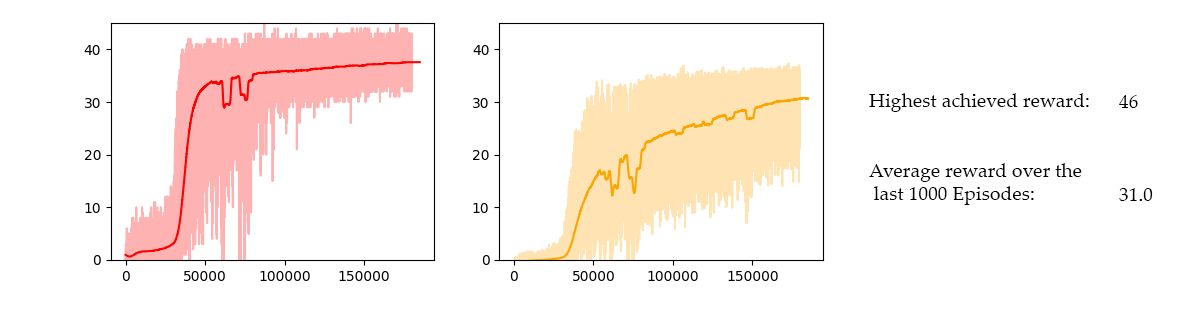
\includegraphics[width=1\textwidth]{Figures/plots/plot_fu_acktr_coord.png}
  \caption{Reward per Episode for the Find Ultralisk Scenario with maximum over all environments(left) and mean over all environments(right)}
  \label{fig:fu_rew}
\end{figure}




\subsection{Find Ultralisk With Creep}
This scenario was considerably more difficult and also more complex with an observation space that was twice as big, which reflects in the reward graphs. Not only did this scenario take longer to learn in general, even after learning the correct strategy the policies learned were somewhat less consistent. This is likely due to the large randomness involved in the observation space as there are many different possibilities for the random placement of the creep patches. 

One interesting detail to note is that looking at the plots of the episode length and comparing them to the reward plot \ref{fig:elength} one can see, that the episode lengths progress much faster and earlier to their maximum value of 240 steps than the rewards. 

\begin{figure}[htb]
  \centering
      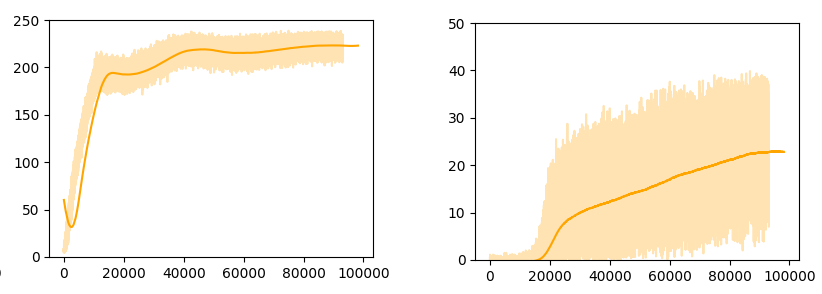
\includegraphics[width=0.8\textwidth]{Figures/plots/fuwc_elength.png}
  \caption{Comparison of Episode length/Episode (left) and Reward/Episode (right) in the Find Ultralisk with Creep Scenario. While the amount of rewards that can be obtained directly correlate to the length of the episode, the length of episode increases much earlier than the rewards after an initial dip.}
  \label{fig:elength}
\end{figure}

Evidently, the algorithm learned very quickly, that it is vital to stay alive and thus stay away from the creep, to get any more rewards at all. Actually getting more rewards by reaching the Ultralisk then only became a secondary objective, that took a while longer to achieve. This is also demonstrated in the decision making of the algorithm during an episode. If for example the algorithm controlled unit has to pass in between two patches of creep that are very close together in order to get to the Ultralisk, the algorithms tends to go back and forth for sometimes 10 to 20 steps in front of and inside of the gap, just to make sure not to touch the creep. After shuffling around for a bit it then heads straight for the Ultralisk. This decision making is even more apparent in the simplified version of this scenario, where the algorithm only has limited movement options. Figure \ref{fig:fu_shuffle} showcases this behaviour in a short sequence of steps that demonstrate part of the back and forth movement of the unit.

\begin{figure}[htb]
  \centering
      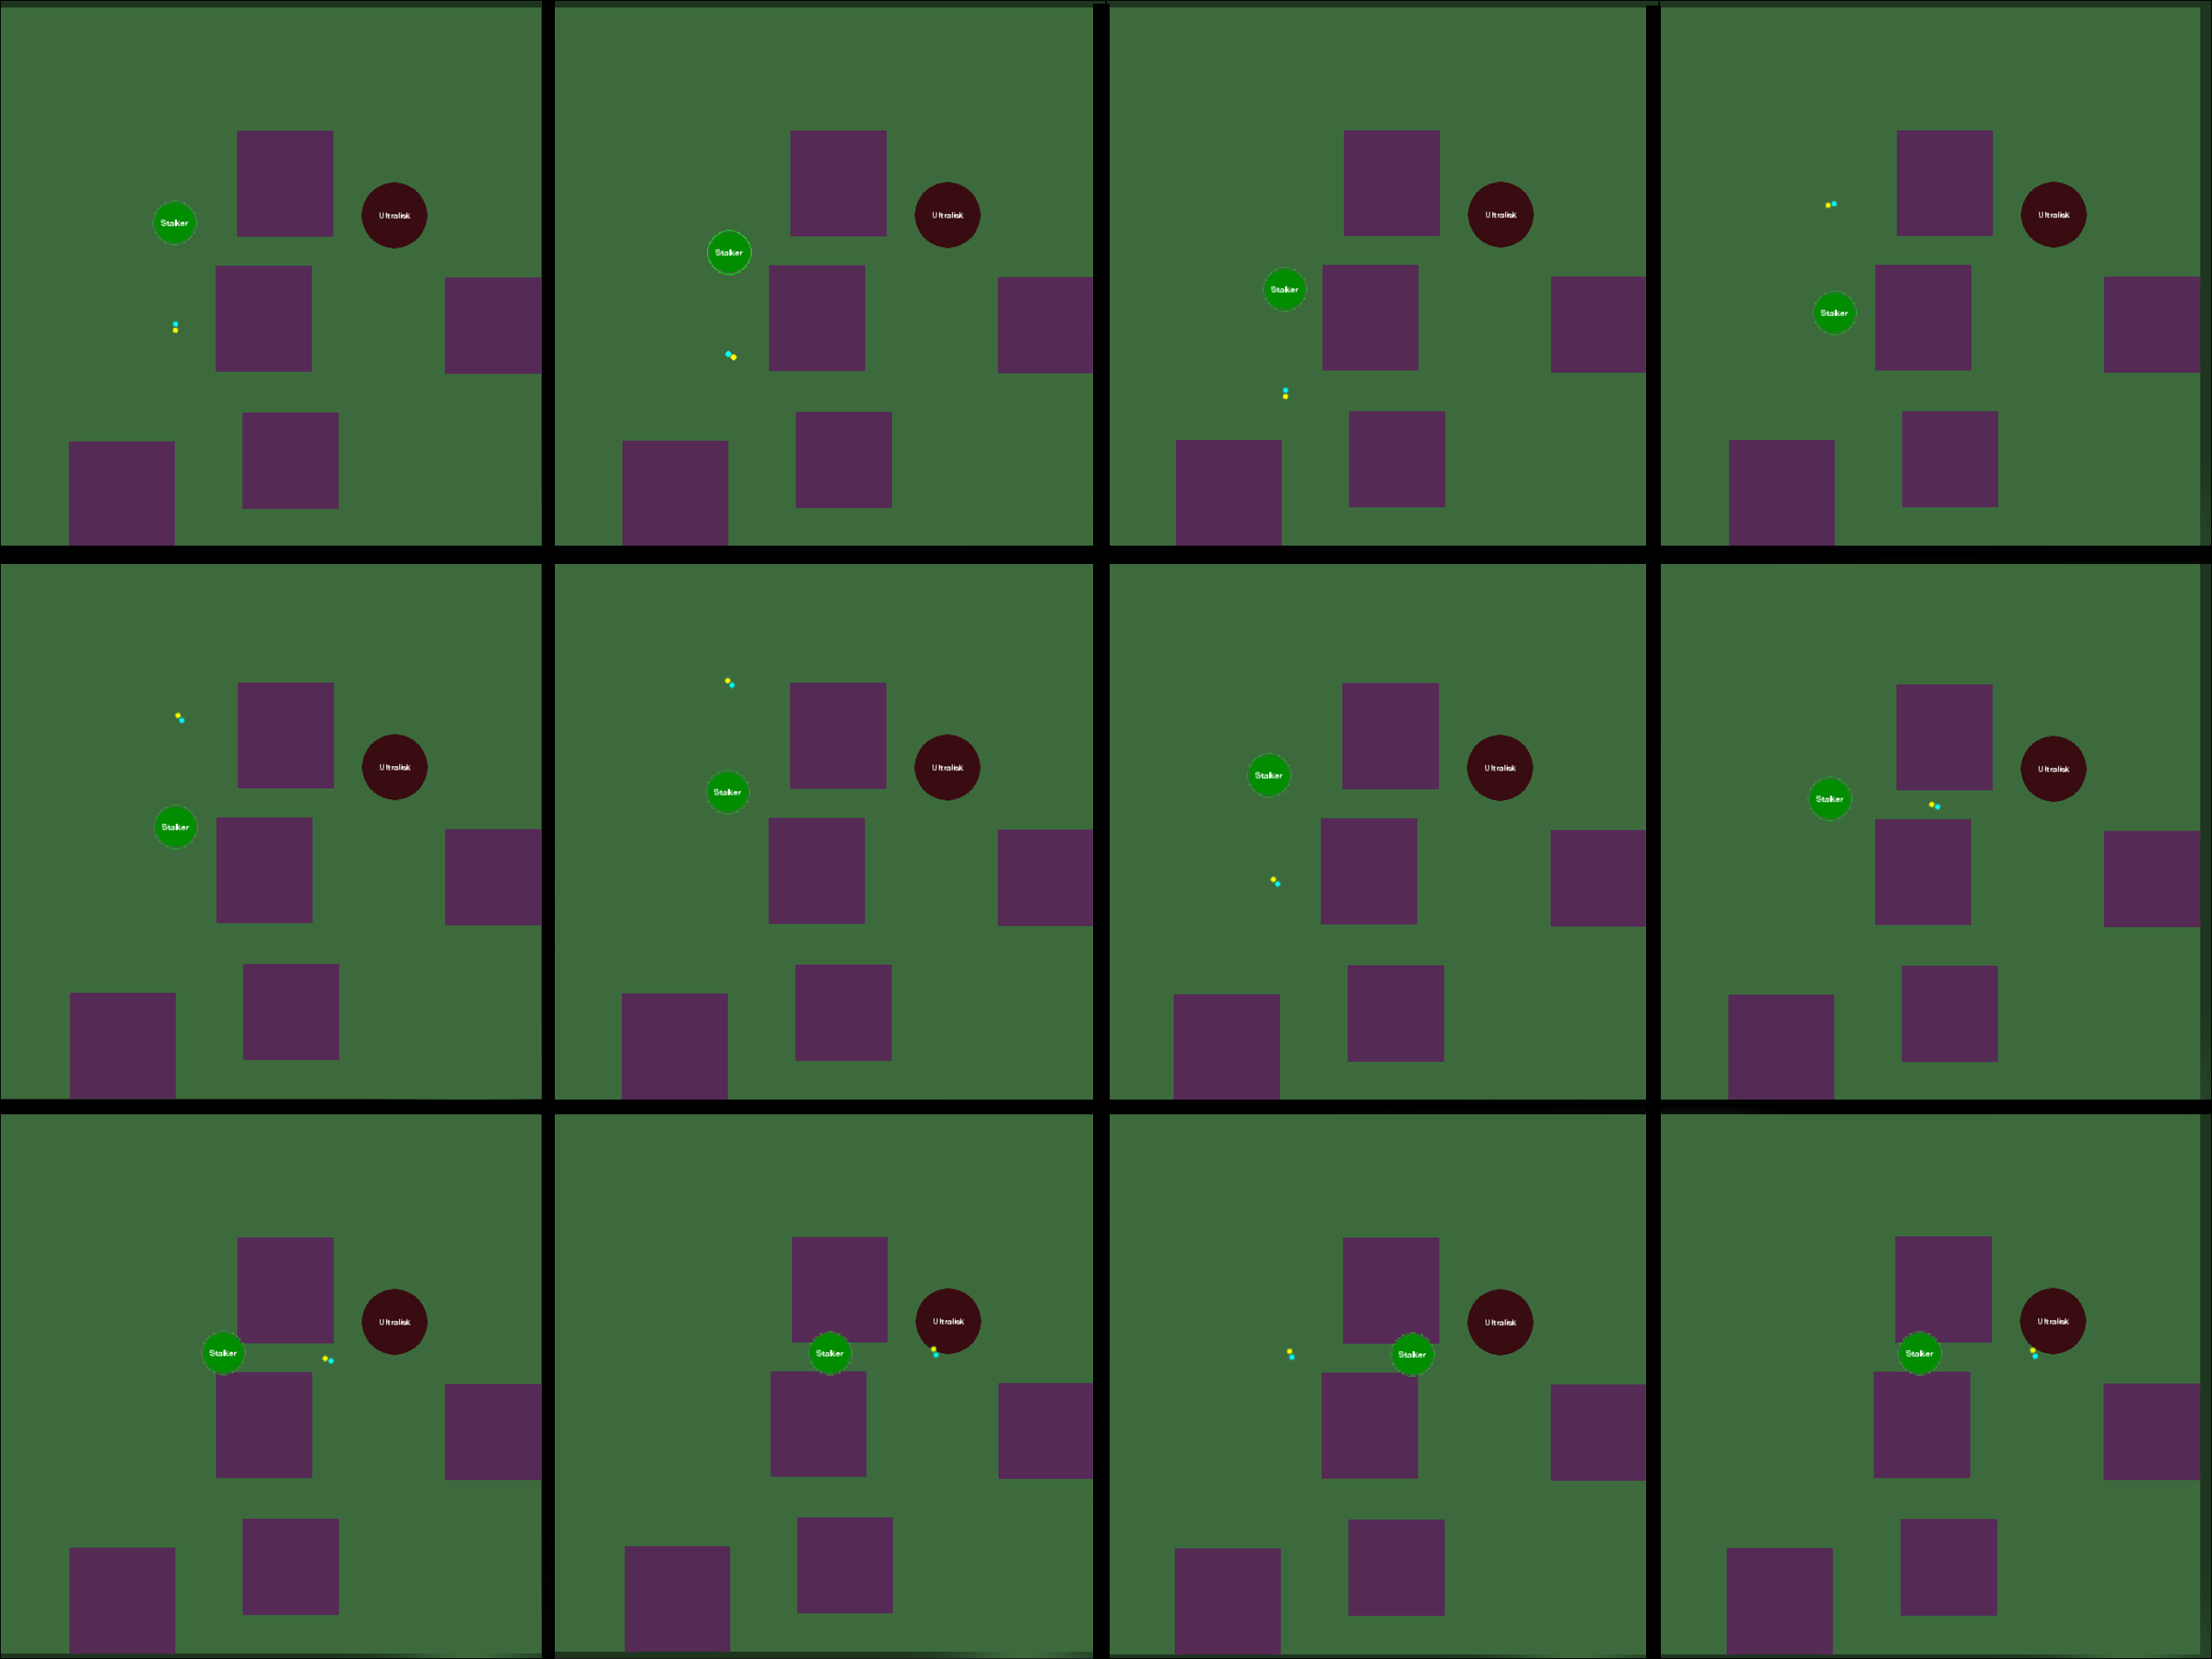
\includegraphics[width=0.8\textwidth]{Figures/fu_sequence.png}
  \caption{Excerpt of ACKTR Behaviour in Find Ultralisk with Creep Scenario when encountering a narrow path to the target. The unit moves back and forth multiple times both in front of and inside of the gap before proceeding to the target.}
  \label{fig:fu_shuffle}
\end{figure}


\subsection{Reaper vs Zergling}
The results of training on the Reaper vs Zergling Scenario show a particularly interesting difference between human play and AI play. All humans that tested this scenario played exactly as was expected: jumping up and down cliffs while attacking the group of enemy units in between jumps, thereby exploiting the terrain. The AI found a much easier solution to the original version of this scenario however. Due to the map being constrained to roughly the screen size there exists a small spot left of the lower ramp that the enemy units can not reach. As the enemy units are melee units, units located in this spot are effectively invincible. The solution of the AI therefore was naturally to move its units to this location as fast as possible and to not execute any further movement commands afterwards. While no human found this simple way of winning it is easy to see why this solution is much easier to learn and execute for the AI than the actual strategy that was expected of it.

\begin{figure}[htb]
  \centering
      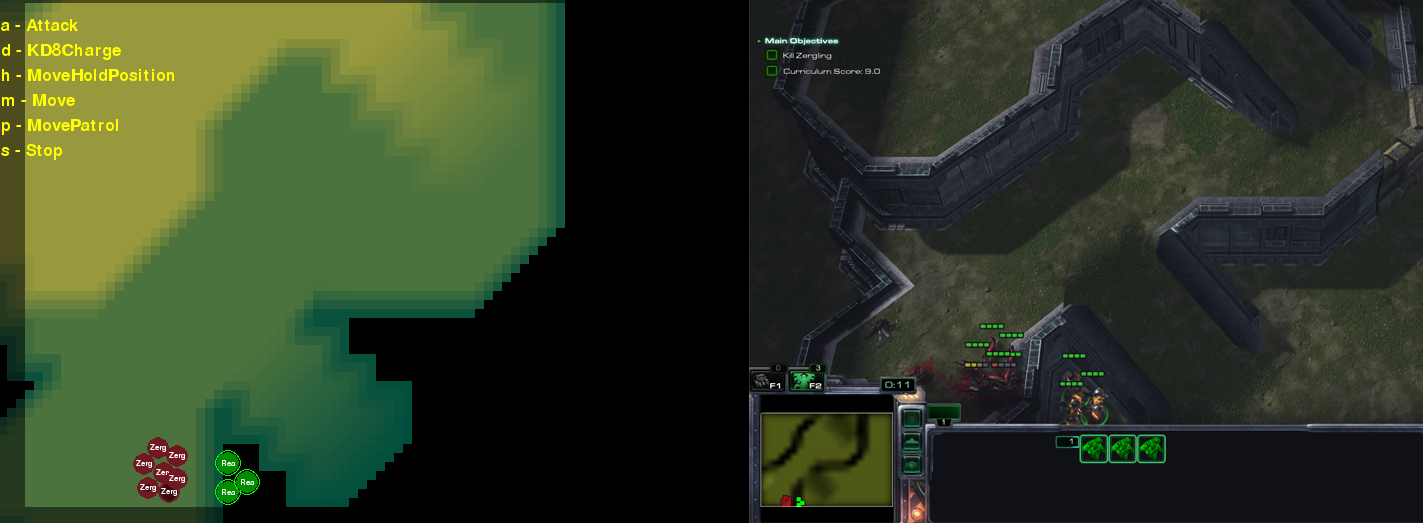
\includegraphics[width=0.8\textwidth]{Figures/rz_badramp.png}
  \caption{AI Strategy for "cheating" the original version of the Reapers vs Zergling Scenario by positioning its units in a location where they can not be reached by enemy melee units. PySC2 debug view left, real game render right.}
  \label{fig:rzstrat}
\end{figure}

In Figure \ref{fig:rzstrat} this strategy can be seen during an episode. The algorithm's units are safely tucked away in between the ramp and the cliff, and the enemy melee units can not reach them. Figure \ref{fig:rzcheat} shows the rewards obtained while learning this "cheating" strategy. While they are still far from the rewards obtained by human players, as the algorithm had problems to execute this strategy consistently, they are much better than the results for the map version that does not allow cheating displayed in Figure \ref{fig:rznocheat}. In that version only very small improvements were made over the random policy. The algorithm did not learn to exploit the terrain to it's advantage and instead simply took small steps away from the enemiy units between attacking them. While this does help a little bit, by giving the algorithm's unit slightly more time before they get defeated, eventually they are overwhelmed by the much faster enemy units. 


\begin{figure}[htb]
  \centering
      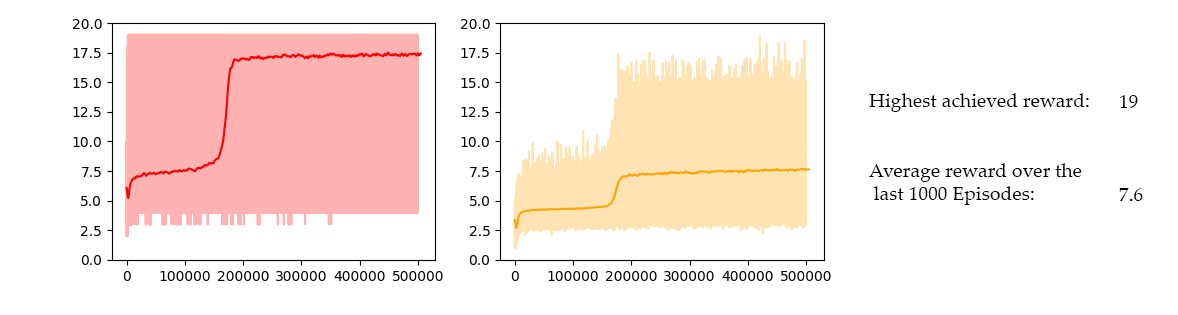
\includegraphics[width=0.8\textwidth]{Figures/plots/plot_rz_acktr_coords_cheat.png}
  \caption{Maximum and Mean Rewards for The ReaperZergling Scenario, in the version of the map that allows the algorithm to "cheat".}
  \label{fig:rzcheat}
\end{figure}

\begin{figure}[htb]
  \centering
      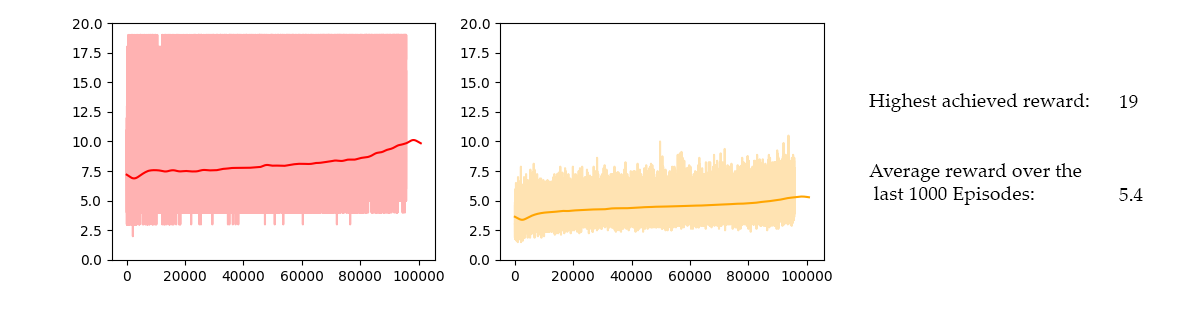
\includegraphics[width=0.8\textwidth]{Figures/plots/plot_rz_acktr.png}
  \caption{Maximum and Mean Rewards for The ReaperZergling Scenario, in the version of the map that does not allow the algorithm to "cheat".}
  \label{fig:rznocheat}
\end{figure}


\subsection{Stalkers vs Roaches}
During conception of the scenarios for this project, this scenario was considered the most difficult to learn by far. Although in comparison with the other real game scenarios of Gateway vs Zerg and Reapers vs Zergling this scenario has a slightly smaller action space and observation space it requires the most challenging strategy to be successful. In contrast to the other scenarios, where each individual action has meaningful impact on the current state in the environment, the strategy for this scenario requires a combination of actions. Namely, the select\_point Action by itself does not change much, but it is required to select wounded units in order to then teleport them to safety using the blink action. Additionally, the difficulty is increased as the requirement placed on the accuracy of screen coordinates is much higher. The Select\_Point Action needs to hit very specific units that are only 3-4 pixels high and wide in order to be effective, while in other scenarios very rough coordinates are enough to achieve close to optimal effects. 

\begin{figure}[htb]
  \centering
      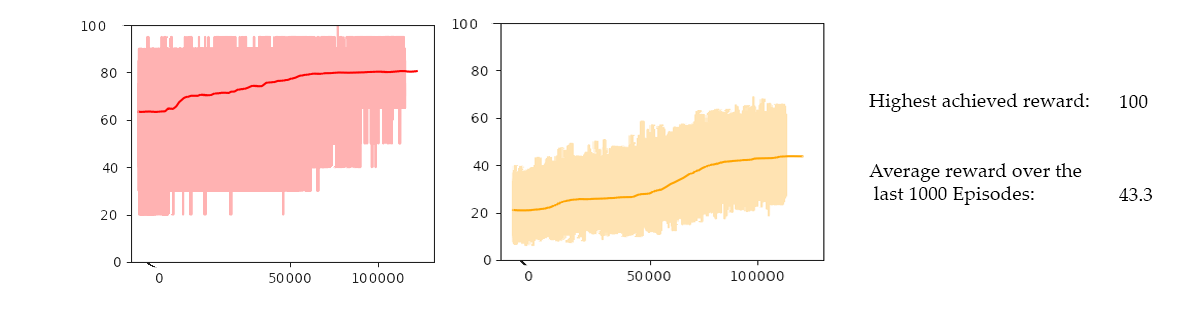
\includegraphics[width=1\textwidth]{Figures/plots/plot_sr_acktr_coord.png}
  \caption{Reward per Episode for the StalkerRoaches Scenario with maximum over all environments(left) and mean over all environments(right)}
  \label{fig:sr_rew}
\end{figure}

As Figure \ref{fig:sr_rew} shows, decent rewards were able to be obtained, in spite of these challenges. In contrast to other scenarios there is no steep reward ascend here, and instead a rather slow increase, that almost plateaus towards the end. Although average rewards are subpar compared to human results, the maximum rewards over all environments show much more promise with rewards of 100 being obtained with considerable regularity. The big discrepency between mean and maximum rewards for this scenario can be attributed to both the fact, that 32 parallel environments were used for training this scenario unlike the 8 environments used for most other scenarios and also to the generally very large inconsistency of the strategy employed by the network. 

The strategy that was learned and is demonstrated by Figure \ref{fig:srstrat} is similar to the strategy of the Reaper vs Zergling scenario in that the algorithm found a way to circumvent the problems of the scenario and instead found a considerably simpler solution. Nonetheless in this case it was not a strategy that exploits a flaw in the design of the scenario and and it is in fact a somewhat suboptimal strategy, that will never be able to achieve full rewards very consistently. What the algorithm has learned, is to effectively never use the select\_point action at all. Instead it relies solely on the blink or teleport action. As the entire army is preselected at the start of each episode, this results in the entire army getting teleported instead of, as intended, singular units. Ideally the teleport location is chosen in a a way that still puts the injured and at risk units at the back of the army, so the core concept of the strategy that was learned is the same as in the human strategy. 

\begin{figure}[htb]
  \centering
      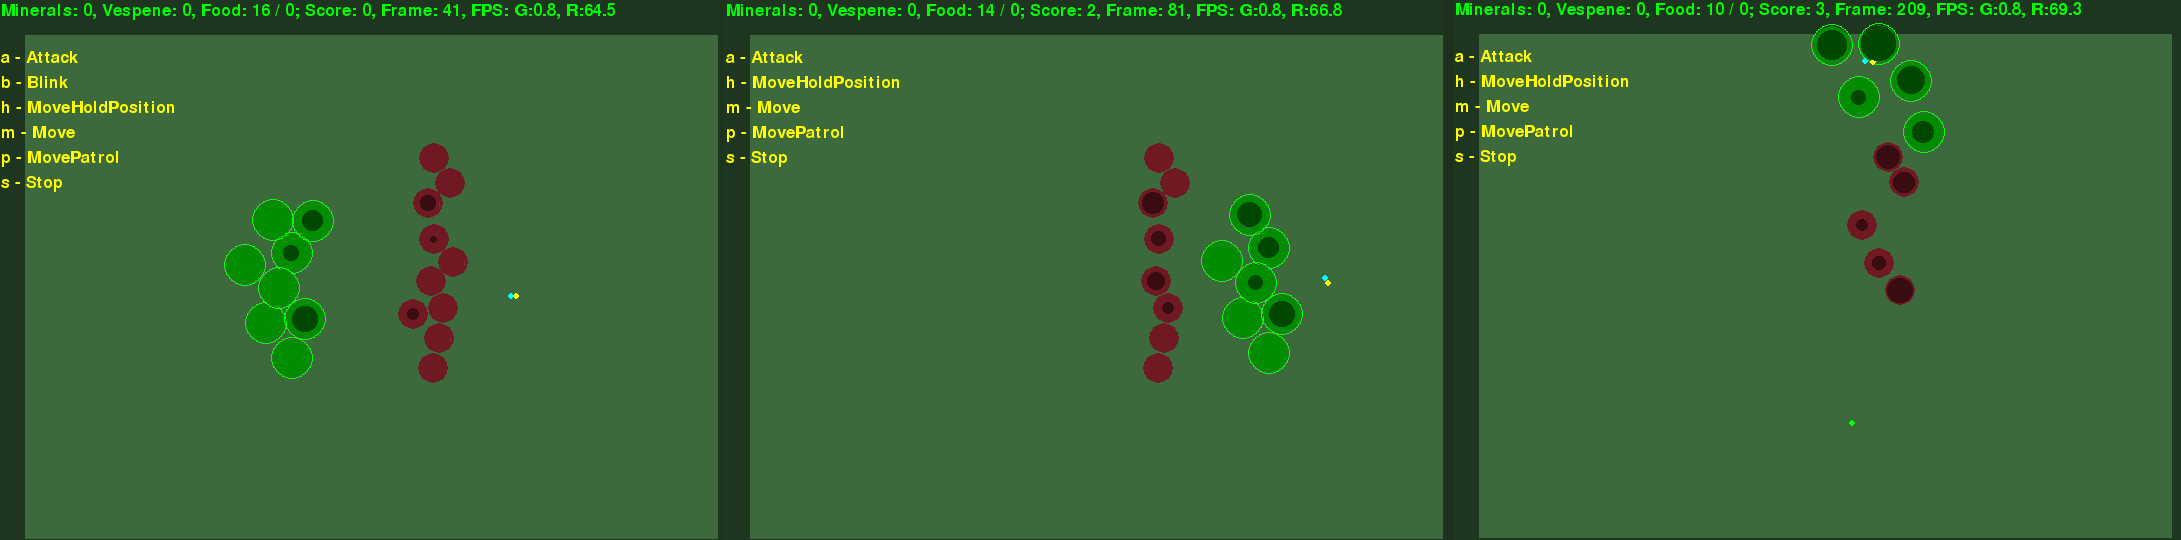
\includegraphics[width=1\textwidth]{Figures/sr_strategy.png}
  \caption{A sequence of select state snapshots demonstrating the strategy that was learned for the Stalkers vs Roaches Scenario. Instead of teleporting single units the entire army is teleported. Increasingly bigger dark green circles on a friendly unit indicate missing health.}
  \label{fig:srstrat}
\end{figure}


Teleporting the army has a few drawbacks however, that preclude it from achieving maximum rewards in most cases. The biggest one is that the blink ability has a considerable cooldown period before it can be used again, which often results in units dying while the ability is still on cooldown. Secondly, executing the blink ability causes all blinked units to stop attacking for a short duration, which makes them more vulnerable and decreases the overall damage that the army is able to inflict. Thirdly it is not always possible to teleport the entire army in a way, that injured units get placed at the back, for example if the enemy army is standing with the back ranks against a wall, effectively wasting the ability. Nonetheless, as can be seen from the reward graph the rewards were still steadily improving at the time the training was stopped. That could mean that the algorithm would not necessarily converge on this suboptimal strategy and might have been able to unlearn this strategy in order to adopt a new one given more training time.   

\subsection{Gateway vs Zerg}
This scenario is definitely the most challenging of the scenarios proposed in this project for human players. One reason for this is that in contrast to the other scenarios there is no clearly definable strategy which, if executed correctly, will always result in maximum rewards. While the general idea is to cut the enemies' army in half and force the enemy to fight your army in small groups using forcefields, this is only a very approximate goal, the path to which is constantly changing, as both armies move around the battlefield. It is also difficult, because it requires a considerable amount of foresight and prediction for, on the one hand determining were enemy routes will follow around the forcefields, and on the other hand managing the available energy of the sentry units in order to not run out of energy by placing forcefields prematurely or unnecessarily. 

The ACKTR algorithm however had little problems with this scenario and managed to gain by far the best results out of the 3 real game scenarios. It was able to not only surpass the novice StarCraft II player'S scores, but is even on par with the advanced player. Additionally surprising was, how consistent the achieved rewards were. In nearly every episode at least 90\% of the possible rewards were achieved.

\begin{figure}[htb]
  \centering
      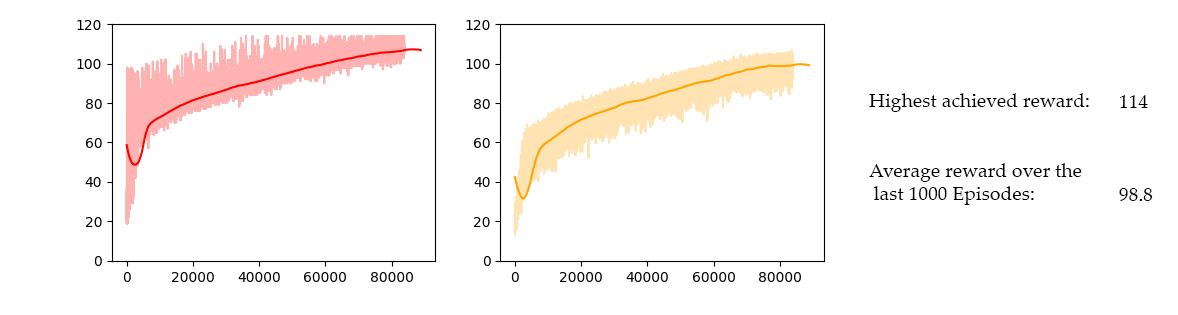
\includegraphics[width=1\textwidth]{Figures/plots/plot_gz_acktr.png}
  \caption{Reward per Episode for the Gateway vs Zerg Scenario with maximum over all environments(left) and mean over all environments(right)}
  \label{fig:gz_rew}
\end{figure}

As Figure \ref{fig:gz_rew} shows, the network actually got worse than random actions for the first few thousand episodes, followed by a short but steep ascend, after which it then slowly and steadily improved until training was stopped after approximately 83000 Episodes per Environment. For this scenario there is largely no difference between mean and max plots as the results were very consistent across environments and on an episode to episode basis.

All of the aforementioned human strategies were learned almost perfectly by the algorithm. It cuts the enemy army in half, and not just randomly, but purposefully in a way that most if not all enemy melee units are on one side and all ranged units on the other for maximum effectiveness. It also conserves energy by placing the forcefields considerably more efficient than was observed in the human tests. Where humans most of the time used 7-8 forcefields very quickly, the algorithm on average only needs 4-5 forcefields to cut the enemy army in half. After that it simply waits and uses the saved energy only if one of the forcefields expires in order to shore up the hole that was left by it or if the enemy units manage to actually get around the existing forcefields. 

\begin{figure}[htb]
  \centering
      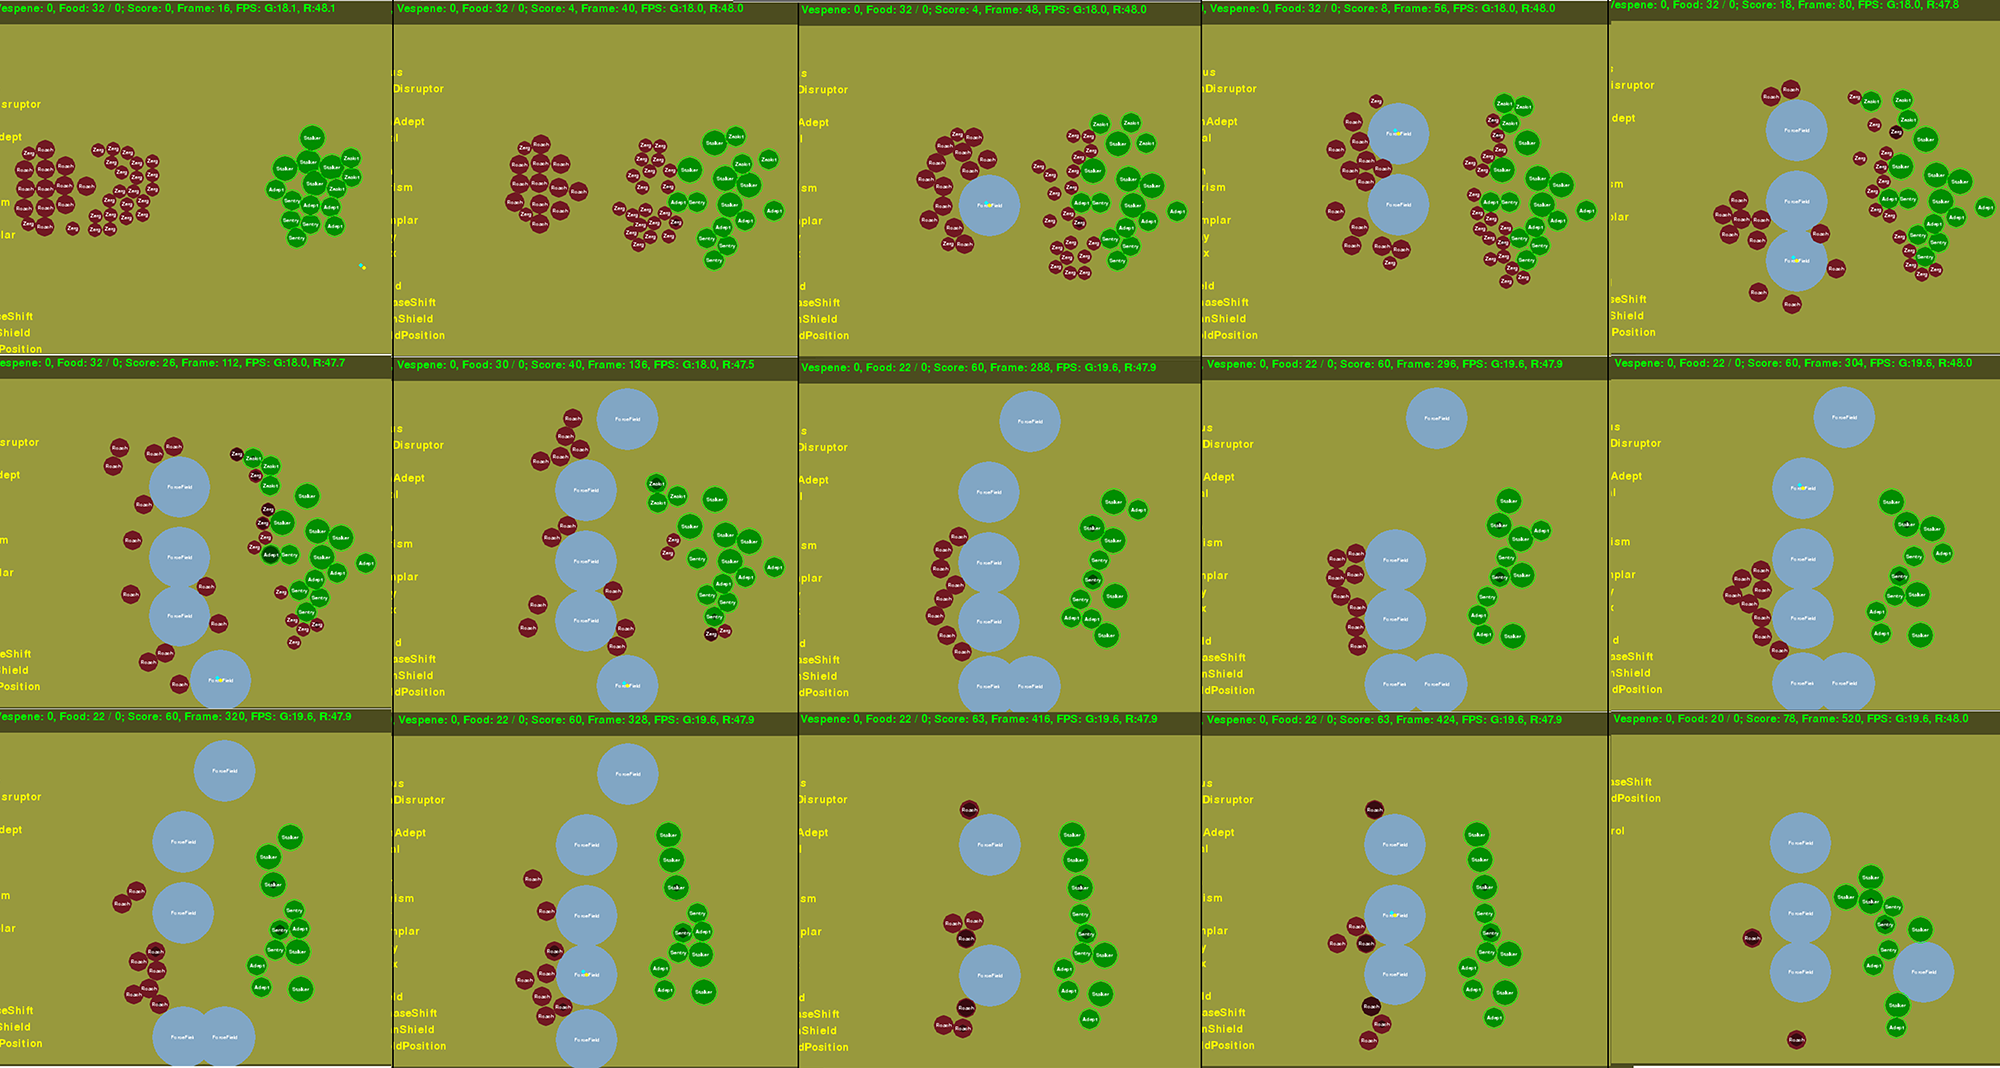
\includegraphics[width=1\textwidth]{Figures/gz_strategy.png}
  \caption{ A Sequence of select state snapshots using a trained model on the Gateway vs Zerg Scenario. The network places the forcefields(blue) strategically to disrupt the enemy army and keep ranged units from attacking the own army}
  \label{fig:gzstrat}
\end{figure}

Figure \ref{fig:gzstrat} illustrates this exact behaviour, showing one episode in which almost maximum rewards were achieved. The only misstep that was made in this episode is right at the end, where a forcefield is placed inside of the players army, but there are not enough enemy units left over to capitalize on this mistake, which is likely why the network has not unlearned or discouraged this behaviour.
\subsection{Scenario Comparison}

\begin{table}[htb]
\centering
\begin{tabular}{@{}llllll@{}}
\toprule
Scenario                 & $s_1$ & \begin{tabular}[c]{@{}l@{}} $s_2$\end{tabular} & \begin{tabular}[c]{@{}l@{}} $p_1$\end{tabular} & \begin{tabular}[c]{@{}l@{}} $p_2$\end{tabular} & \begin{tabular}[c]{@{}l@{}}$p_3$\end{tabular} \\ \midrule
FindUltralisk            & 46                 & 31.0                                                                                                         & $\sim$92\%                                                                                    & 68\%                                                                                         & 64\%                                                                                            \\
FindUltraliskWithCreep   & 46                 & 23.2                                                                                                         & $\sim$100\%                                                                                   & 62\%                                                                                         & 54\%                                                                                            \\
GatewayZerg              & 114                & 98.8                                                                                                         & 92.3\%                                                                                        & 156\%                                                                                        & 99\%                                                                                            \\
StalkerRoaches           & 100                & 43.3                                                                                                         & 100\%                                                                                         & 72\%                                                                                         & 45\%                                                                                            \\
ReaperZergling(Cheating) & 19                 & 7.6                                                                                                          & 100\%                                                                                         & 44\%                                                                                         & 40\%                                                                                            \\
ReaperZergling           & 19                 & 5.4                                                                                                          & 100\%                                                                                         & 31\%                                                                                         & 28\%                                                                                            \\ \bottomrule
\end{tabular}
\captionsetup{singlelinecheck=off}
\caption[]{Summary of Scenario evaluations. \\ Column Definitions:
\begin{itemize}
\item $s_1$ - Maximum Score obtained
\item $s_2$ - Average Score obtained over last 1000 Episodes across all Environments
\item $p_1$ - Percentage for $s_1$ of maximum Score possible
\item $p_2$ - Percentage for $s_2$ of novice Player baseline
\item $p_3$ - Percentage for $s_2$ of advanced Player baseline 
\end{itemize}
}
\label{tab:scen_eval}
\end{table}

Table \ref{tab:scen_eval} compares the best results that were able to be obtained in each scenario. Both the maximum scores ($s_1$, $p_1$) and an average over 1000 Episodes after a policy was learned ($s_2$) are compared and put into the context of human player's results ($p_2$, $p_3$). The percentages calculated for the maximum reward $p_1$ are adjusted for the minimum possible reward as well, where it differs from 0. This makes an especially big difference in the GatewayZerg scenario, where the minimum reward is already ca. 45.  

Some of these results conform roughly with the expectations that were held at the beginning of this thesis. The Find Ultralisk and Find Ultralisk with Creep scenarios were solved with considerable success, albeit not quite as consistently as either of the human players. The Stalker vs Roaches scenario, as expected, posed much more of a challenge and the algorithm was not able to learn the "correct" strategy, which shows in the average rewards it obtained. Nonetheless, even it's suboptimal policy managed to achieve maximum rewards at least sometimes.

There were also big surprises however. The algorithm performed much better than expected in the Gateway vs Zerg scenario. It being the most difficult scenario for humans the algorithm was expected to have quite a few problems with it as well, but it managed to become just as good as the advanced human player. It is particularly surprising how consistently high scores were achieved in comparison with all other scenarios, where even after learning the optimal strategy the obtained rewards span the entire range of possible rewards in the environment. The reason this scenario might be easier for reinforcement learning algorithms than the other scenarios is that it exhibits slightly less randomness for a computer at least. A large part of the randomness and difficulty felt by humans in this scenario comes from not being able to predict the movement of enemy units around the forcefields during split second decision making. This pathing is actually deterministic however. Therefore if an algorithm is able to predict this movement, this scenario becomes much easier, as there are fewer differences between states of different episodes, if similar movement patterns can be forced by similar forcefield placement.

A surprise in the opposite direction were the results of the ReaperZergling scenario. Initially thought to be the easiest of the three competitive scenarios it turned out to be the scenario the algorithms had the most difficulty with. As can shown by the results in table \ref{tab:scen_eval} even with cheating the algorithm only managed to obtain 44\%/40\% of the human players' scores. This is due to the fact that, while sitting in the corner where the units cannot be reached easily guarantees a high score, getting to that spot is still somewhat difficult and could not be done consistently. This is likely owed to the enemies' very fast movement being hard to predict because of the unorthodox terrain and pathing mechanisms. Without the possibility of simply hiding the algorithm faired even worse, achieving only 31\%/28\% of human scores. In both versions the algorithm was able to achieve the maximum score of 19 every once in a while though.

In conclusion the FindUltralisk and FindUltraliskWithCreep scenarios do the job of introductory scenarios quite well, but the GatewayvsZerg scenario works just as well if not better, while also being a scenario that reflects the actual game. These results also show, that scenarios that are somewhat difficult for human players can be very easy for reinforcement learning algorithms and vice versa.

\section{Algorithms}
\label{sec:eval_algo}

This section will compare the three algorithms that were used in this project in their usefulness for StarCraft II Reinforcement Leaning. This section however was hit hardest by the resource and time constraints, as after trying to solve all scenarios using the ACKTR algorithm there was not enough time to tune both other algorithms adequately for all of them. This means that some scenarios, especially the more difficult ones, were left entirely unsolved by the A2C and A3C algorithms.

From OpenAI's blog post \citep{openaiblog-a2c} and other sources the initial expectation was that ACKTR will outperform A2C and A3C by a considerable margin. In the few comparisons that can be made, this expectation was not only confirmed, but the differences seem to be even greater than anticipated. The easiest scenario, Find Ultralisk, is the only scenario where all three algorithms were able to obtain close to optimal results with any kind of consistency. Nonetheless, it already highlights one of the big problems with the A3C implementation. After the A3c algorithm was able to learn a policy that achieves decent rewards it, sometimes almost instantly, unlearns this policy a few hundred or thousand episodes later as seen in Figure \ref{fig:a3c_unlearn}. This happens even with relatively small learning rates, that should only allow small adjustments to be made to the network weights, which might indicate a bug in the implementation, but that could not yet be determined.    
\begin{figure}[htb]
  \centering
      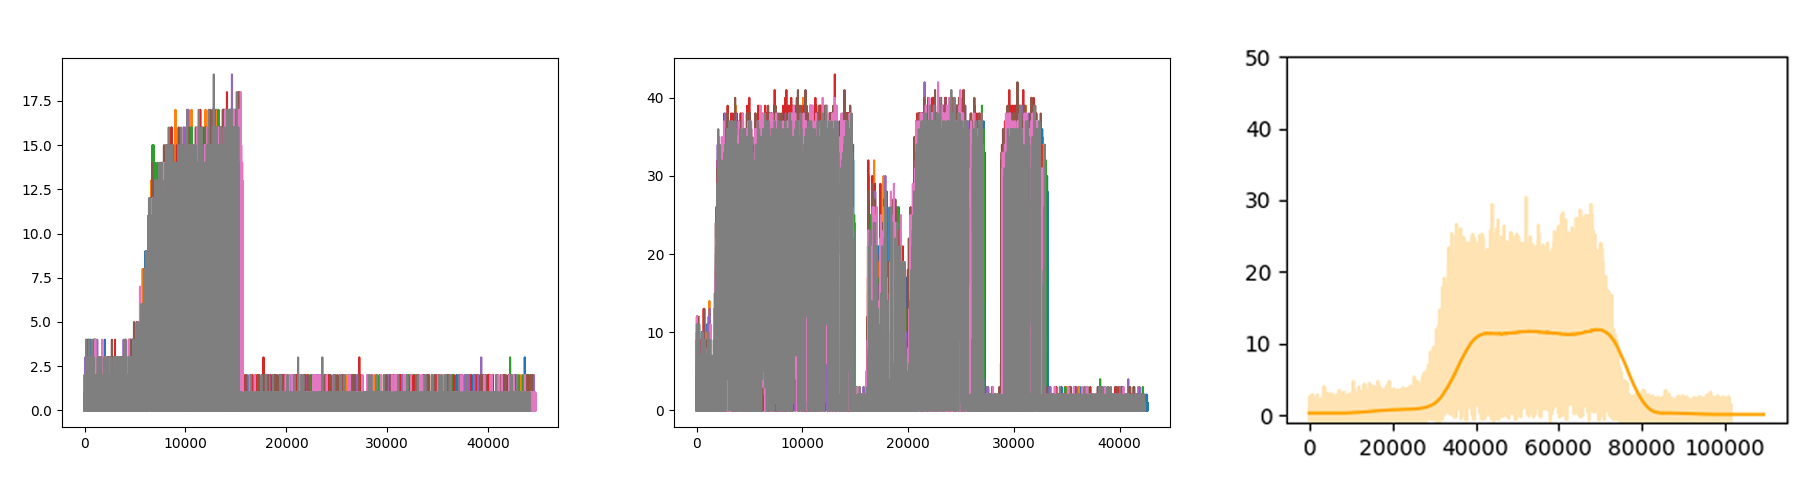
\includegraphics[width=1\textwidth]{Figures/plots/a3c_unlearning.png}
  \caption{Different examples of the problem of policy fragility in the A3C Algorithm. Scenarios from left to right: FindUltralisk(simplified), FindUltraliskWithCreep(simplified), FindUltraliskWithCreep(proper). The rightmost plot also shows how much worse the A3C performed in general, with an average score of only 12 points during it's peak in  the FindUltralisk Scenario}
  \label{fig:a3c_unlearn}
\end{figure}

The GatewayZerg scenario, although quite easy for the acktr algorithm, could not be adequately learned by the A3C algorithm, as shown by Figure \ref{fig:gz_a3c}. The policy learned is only a very slight improvement over the random policy and is not comparable with the human players.

\begin{figure}[htb]
  \centering
      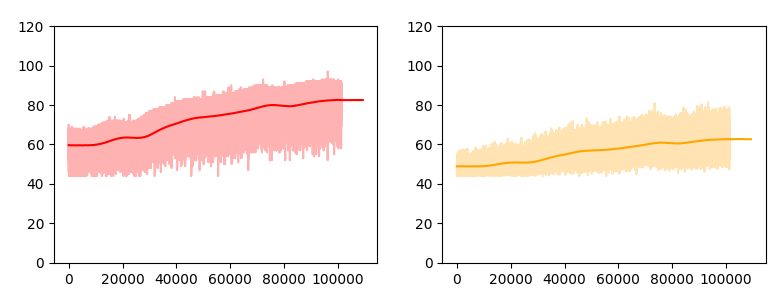
\includegraphics[width=0.8\textwidth]{Figures/plots/gz_a3c.png}
  \caption{Performance of the A3C algorithm in the GatewayZerg scenario. While small improvements were made, the policy obtains still largely random scores.}
  \label{fig:gz_a3c}
\end{figure}

For the ReaperZergling and StalkerRoaches scenarios no meaningful policy could be learned at all by the A3C algorithm.

The A2C algorithm did not exhibit the unlearning problem of the A3C algorithm and for the FindUltralisk scenario in it's simplified variant was even able to beat the ACKTR algorithm with the scores depicted in Figure \ref{fig:a2c_fu}. This is the only scenario that the A2C algorithm successfully learned however, and the fact that it beat the ACKTR algorithm is likely due to differently tuned hyperparameters and not an indicator that the A2C algorithm is superior.

\begin{figure}[htb]
  \centering
      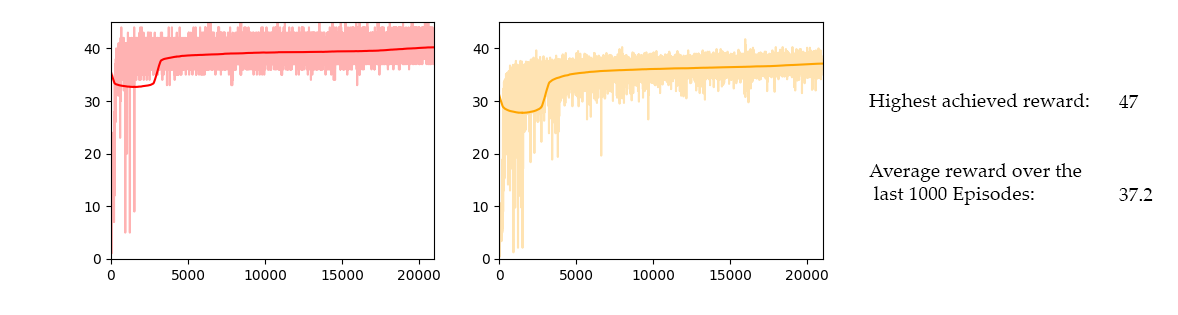
\includegraphics[width=1\textwidth]{Figures/plots/a2c_fu.png}
  \caption{Performance of the A2C algorithm in the FindUltralisk scenario in it's simplified variant. The peak average reward of 37.2 beats even the ACKTR algorithm that only managed 32(cf. Figure \ref{fig:simplevs_fu}). }
  \label{fig:a2c_fu}
\end{figure}

Nonetheless, even the FindUltraliskWithCreep scenario posed very big problems for the A2C algorithm, where it only managed to learn not to step on creep surfaces therefore obtaining exactly 0 reward points in each episode. This was the case in both the simplified variant and using screen coordinates. For this reason no other scenarios were attempted with this algorithm.

One big advantage of the ACKTR algorithm seems to be that it is much less dependent on very precise hyperparamater tuning than A2C and A3C as far as the learning rate is considered. As illustrated in section \ref{sec:lr} atleast for the FindUltraliskWithCreep scenario, there exists a wide range of learning rates that result in decent performance, whereas with the A3C algorithm for example adjustments with precision of $10^{-5}$ were needed to exhibit any information gain at all. 

\section{Simple vs action arguments}
\label{sec:eval_aa}
The next comparison to be done is between the different action representations for the policy, specifically between the simplified versions and the versions featuring screen coordinates.
This comparison can not fully be done over all scenarios, and for this reason this section will only feature scenarios that have a simplified variant. 

Originally a third strategy was meant to be added to this comparison, the flattening approach, which simply merges arguments and actions into a one dimensional array. This would have been a good measure for determining how beneficial it is to separate action and screen coordinate outputs from the neural network, but this part of the comparison could not be completed in time for this thesis.

In general it can be said, that the simplified variants were learned faster and more smoothly than the variants making use of actual coordinates. The simplification is not without drawbacks however, as in the end most models using action arguments were able to obtain at least slightly higher rewards more consistently than the models trained with the simplified actions. This is largely owed to the fact that  units can simply be moved more efficiently with precise coordinates in comparison to the grid like movement they are constrained to by the abstract actions. Figure \ref{fig:simplevs_fu} shows these differences in the FindUltralisk scenario.

\begin{figure}[htb]
  \centering
      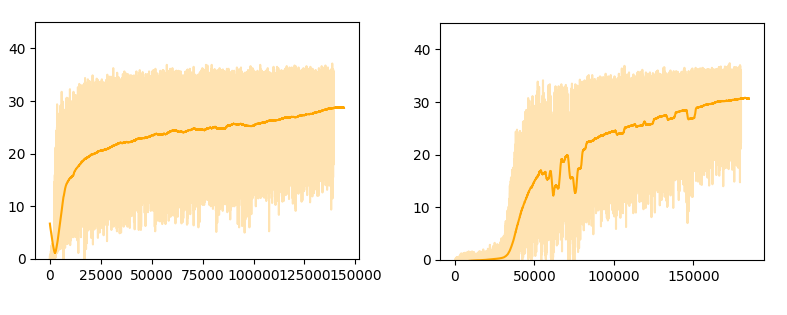
\includegraphics[width=0.8\textwidth]{Figures/plots/acktr_fu_simplevs.png}
  \caption{Comparison of simplified version(left) and version with action arguments(right) in the FindUltralisk scenario.}
  \label{fig:simplevs_fu}
\end{figure}

The results for the FindUltraliskWithCreep scenario depicted in Figure \ref{fig:simplevs_fuwc} are similar. The test run for the simplified version sadly had to be terminated prematurely, but the rewards seemed to mostly stagnate so this comparison still holds. The simplified variant again was learned much faster but with less maximum and average rewards in the long run.
\begin{figure}[htb]
  \centering
      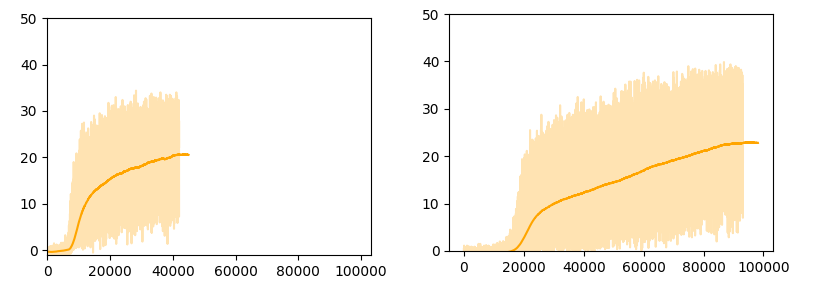
\includegraphics[width=0.8\textwidth]{Figures/plots/fuwc_simplevs.png}
  \caption{Comparison of a short run of simplified version(left) and version with action arguments(right)in the FindUltraliskWith scenario.}
  \label{fig:simplevs_fuwc}
\end{figure}

The Reaper vs Zergling Scenario exposes an even larger problem with the abstracted actions of the simplified versions. Due to the way StarCraft II's internal pathfinding algorithm determines the actual path that the units take in order to get to the coordinate specified by the player during any action that requires movement, the grid-like movement can lead to very unintuitive results, when there are obstacles or terrain changes in the path of the unit. This is because the pathfinding algorithm will automatically choose an optimal path around all obstacles and also up or down different terrain height levels.

An additional problem for the simplified actions that arises in any scenario involving different terrain heights is the fixed distance, that the unit is ordered to move in each step, which increases the discrepancy even further between where the unit is ordered to move to and where the pathfinding algorithm actually moves it towards in the next step.


\section{Impact of Sample Diversity by Environment Parallelisation}
While not strictly related to the StarCraft II environment, for the purpose of performance testing it was determined how much the diversity of samples gained by using a number of parallel environments improves sample efficiency. This was considered important, as training slows down with too many environments meaning this sample efficiency has to be weighed against time efficiency. Tests were done on the somewhat easy Find Ultralisk With Creep Scenario to ensure that even if missing sample diversity is a large problem for the ACKTR algorithm, it should still able learn at least something. The number of parallel environments tested are 1, 2, 8, 16 and 32.

For this evaluation the plots were generated slightly differently than before. In order to better compare the results no average was made across the environments, and instead the results of each environment are merged into one plot in a zipper like manner. Looking at the graphs one can still see a large difference in the number of episodes, that were run in each test, but this can be attributed to the varying length of episodes, all tests were run for exactly 80 million time steps.

\begin{figure}[htb]
  \centering
      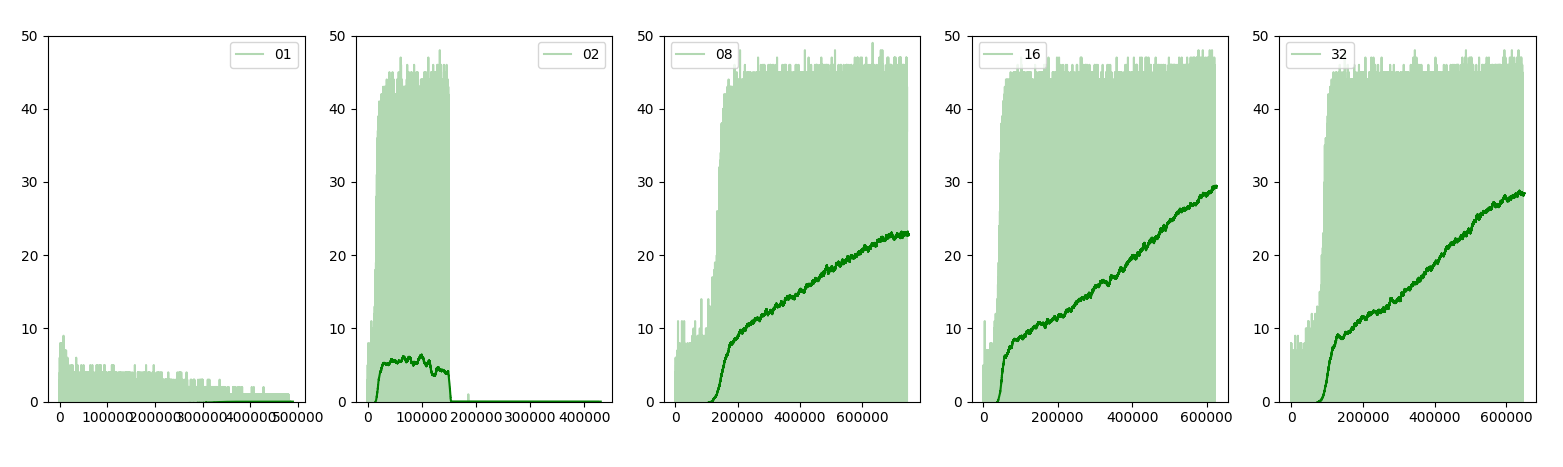
\includegraphics[width=1\textwidth]{Figures/plots/acktr_diversity.png}
  \caption{Effect of the number of parallel environments on the training process of the ACKTR algorithm. Tested on the Find Ultralisk With Creep Scenario using Action Coordinates. x-Axis: Episode number, y-Axis: End of Episode Reward}
  \label{fig:acktr_diverse}
\end{figure}

Figure \ref{fig:acktr_diverse} shows the result of these tests. These graphs make quite clear, that sample diversity is in fact very important for the ACKTR algorithm. Using only very few  parallel environments might even prevent learning entirely, as shown by the test run with only 1 environment. With 2 environments there was some success at first, almost mirroring the initial reward ascend of the other test runs, but then quickly plateaued and even unlearned everything after a short time, showing that it is much less robust. \\ The difference between the other 3 test runs is much smaller, but still considerable. Utilizing 16 or 32 parallel environments enabled the algorithm not only to learn faster, but also reach higher overall rewards and consistency in comparison with 8 environments, which were used for almost all tests over the course of this thesis. These results indicate, that choosing the number of environments is not only a question of sample efficiency vs time efficiency, but that it might be necessary to utilize a very high amount of parallel environments, to learn an optimal policy.


\section{Impact of different learning rates}
\label{sec:lr}
As the learning rate was the main hyperparameter that was tuned over the course of this project this section contains an analysis how different learning rates affected training in these environments. Tested was only the ACKTR algorithm and tests were made starting with a learning rate of 0.5 which was progressively divided by 10 for each further test. All tests were made on the relatively easy Find Ultralisk With Creep Scenario to ensure, that most of these learning rates get a result, and all tests ran for 80 million steps. Using a relatively easy scenario also shows that using too small of a learning rate can also result in no knowledge gain at all. Figure \ref{fig:acktr_lr} demonstrates this. 

\begin{figure}[htb]
  \centering
      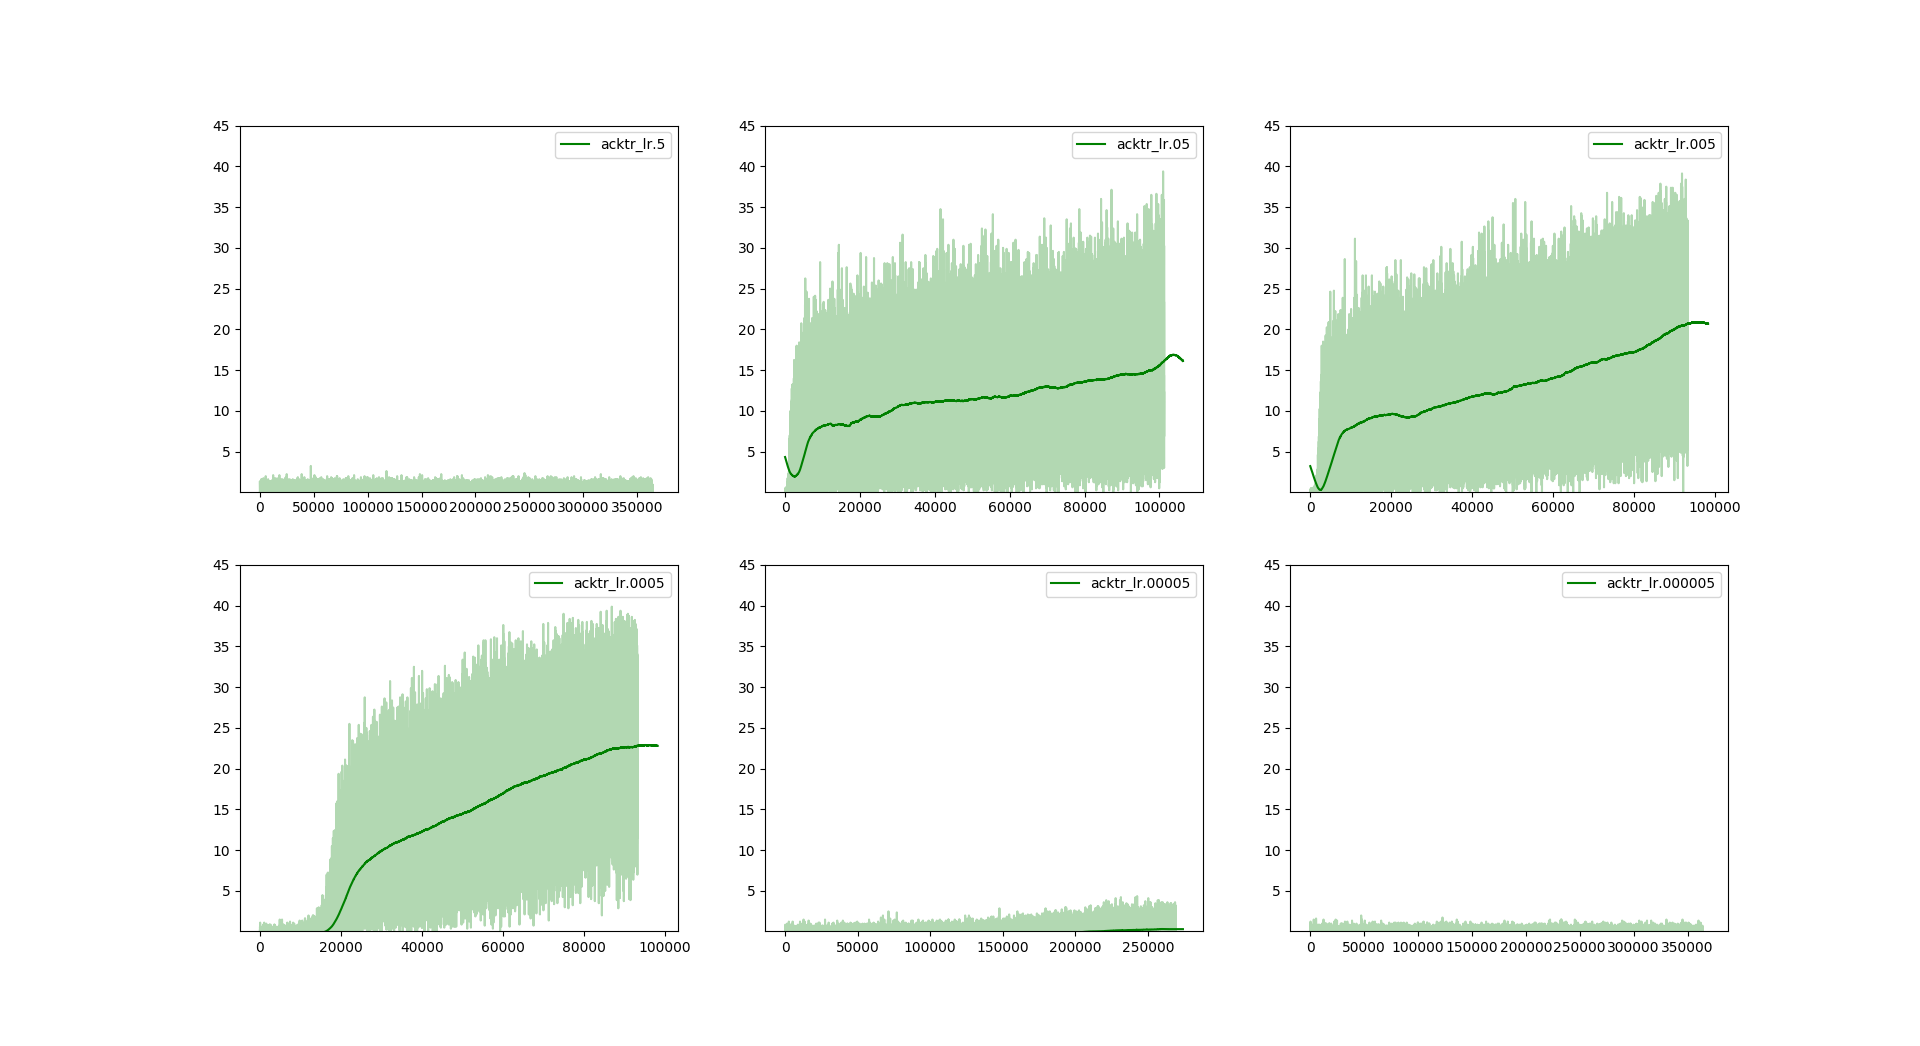
\includegraphics[width=1\textwidth]{Figures/plots/acktr_lr.png}
  \caption{Effect of different learning rates on the training process of the ACKTR algorithm. Tested on the Find Ultralisk With Creep Scenario using Action Coordinates. x-Axis: Episode number, y-Axis: End of Episode Reward}
  \label{fig:acktr_lr}
\end{figure}

In this specific scenario only learning rates between 0.05 and 0.0005 result in any training at all. The best result was achieved using the 0.0005 learning rate, where the reward ascend is very smooth and the highest overall rewards were experienced. Nonetheless the rewards were gained much later than when utilizing higher learning rates,  as for the first about 18000 episodes per environment no rewards were achieved at all, whereas higher learning rates achieved noticeable rewards almost immediately.Their reward ascend is more erratic and slowed down considerably after an initial period of very steep gains however.

In concurrence with these findings the goal for learning the other scenarios optimally was to find he lowest possible learning rate, that still results in learning in a reasonable amount of steps.  


\section{Impact of a state history}
This section compares 2 test runs on the Find Ultralisk with Creep Scenario. One with only a single timestep functioning as the state of the environment, and the other utilizing a history of 4 states.

\begin{figure}[htb]
  \centering
      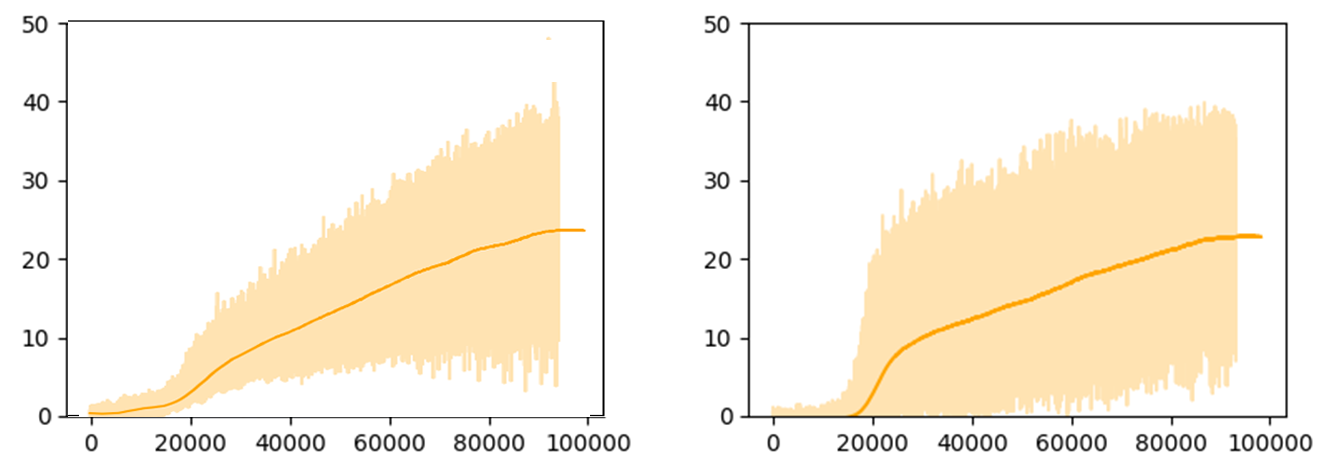
\includegraphics[width=1\textwidth]{Figures/plots/fuwc_history.png}
  \caption{Comparison between utilizing a history of 4 timesteps(left) as observations with a single timestep state(right). Tested on the Find Ultralisk With Creep Scenario using Action Coordinates. x-Axis: Episode number, y-Axis: End of Episode Reward}
  \label{fig:acktr_history}
\end{figure}

As Figure \ref{fig:acktr_history} shows, the end results of both test runs are not substantially different, although the end rewards were slightly higher while using a state history. The largest difference is, that the training curve was smoothed out a considerable amount and results have become somewhat more consistent. This improvement in consistency became much smaller towards the end of the training run however, and in the end they are both almost equally inconsistent. 

As the player in the FindUltraliskwithCreep Scenario does not especially benefit from knowing the last few states, which is also the case for all other scenarios in this thesis, this rather small difference between state history and no state history was more or less expected. 
Because training with the state history took more than twice as long one can conclude, that if the specific scenario to be trained does not necessitate the usage of a state history, or there is some obvious information gain one should likely elect not to use such a state history.  


\section{Impact of Learning from Replays}
The attempt to incorporate human replay experiences into the training process did not go as well as had been initially hoped. 
Both the strategy to slowly add replay samples over time, and the strategy to dump all human experiences before the actual reinforcement learning process begins did not manage to improve the performance or conversion properties of the A3c algorithm in the FindUltraliskWithCreep Scenario.

While the "kick-start" strategy had almost no effect in all cases even when feeding the experiences into the network multiple times, the other strategy did even worse by lowering performance or even preventing training entirely for any but very slow percentages of human replays added. Figure  \ref{fig:a3c_replay} shows a comparison between regular training and the "kick-start" strategy. The largest difference is, that using the human replay experiences the algorithm managed to retain a proper policy for a slightly longer time than without, before unlearning it. This effect however, is largely random and can also be found between multiple runs without replay experiences and can therefore not be seen as an improvement. 

\begin{figure}[htb]
  \centering
      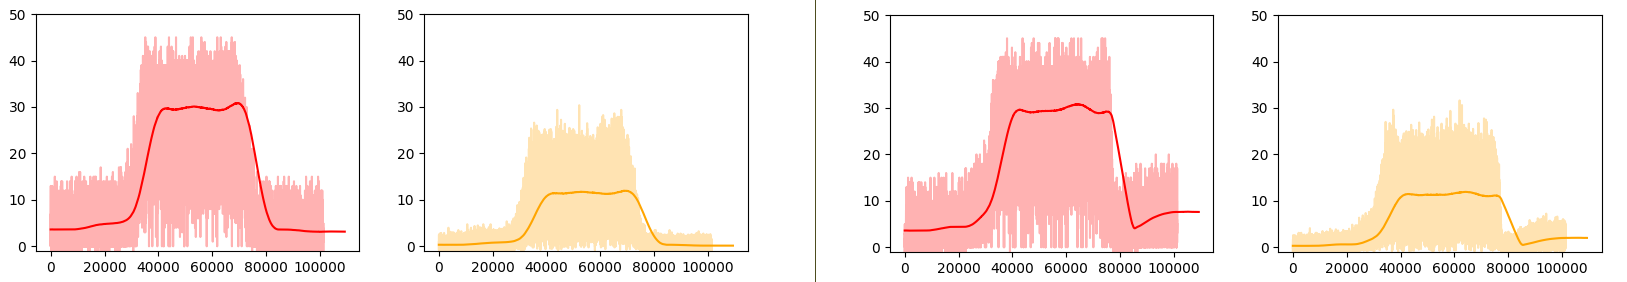
\includegraphics[width=1\textwidth]{Figures/plots/a3c_fuwc_replays.png}
  \caption{Comparison between a test run with added human replay experiences(right) and a standard test run(left) on the Find Ultralisk With Creep Scenario utilizing the A3C algorithm}
  \label{fig:a3c_replay}
\end{figure}

The second scenario that this was attempted on was the ReaperZergling scenario, where the A3c algorithm was not able to learn any meaningful policy without the human experiences and it was hoped, they could change that. Nonetheless, no improvements could be made in this scenario either.

There are multiple reasons that could have led to the failure of this attempt. The largest problem is likely the comparatively insignificant amount of human data of only 1400 steps that was recorded for these tests compared to the 80 million steps done during normal training. For the Find Ultralisk With Creep Scenario they make up only around 30 episodes. In contrast, the a3c algorithm needed around 1000 times more episodes to learn a meaningful policy during regular training. It is therefore easy to see, why they would only have little recognizable impact.

The strategy of slowly adding samples over time adds many more human samples to the network by duplication, which alleviates the previous problem, but introduces a new one. Having tens of thousands or even hundreds of thousands of samples out of the same small set of samples likely introduces overfitting to these exact state spaces. This might also hinder exploration by making the policy more deterministic, counteracting the entropy.

The "kick-start" strategy has one additional drawback, due to the importance of the current value function estimate for calculating the discounted rewards. As all samples are added before the actual training, the value function estimate of the neural network is still largely random or a very rough estimate at best as more of the samples are added. This can not give an accurate representation of the discounted reward.





% Chapter 1

\chapter{Closing Remarks} % Main chapter title

\label{chap_closing} % For referencing the chapter elsewhere, use \ref{Chapter1} 

%----------------------------------------------------------------------------------------
\section{Conclusion}
With the help of the combat scenarios provided with thesis it was demonstrated, that modern reinforcement learning algorithms are indeed able to learn close to optimal policies comparable to expert human players on real scenarios directly taken from the competitive 1 vs 1 mode of StarCraft II. This thesis also highlighted some of the challenges however. On the one side there is the technical aspect of the not quite finished PySC2 framework and the sheer amount of computing power necessary for learning in such a complex environment. On the other side are the challenges brought about by StarCraft II itself, like the vast action- and observation spaces and the complexity of even simple aspects of the game.

This thesis also illustrated that reinforcement learning algorithms do not need to necessarily imitate human strategies and can instead develop their own interesting ways to solve scenarios, that a human might not think about, as showcased by finding the possibility of "cheating" in the ReaperZergling scenario or the simplified strategy employed in the StalkerRoaches scenario.

In general it was established, that even this small excerpt of the game consisting solely of small unit combat holds very unique and interesting possibilities for building environments for reinforcement learning algorithms to be tested on. 

\section{Future Work}
This thesis has barely scratched the surface of what StarCraft II offers as a reinforcement learning environment. Even if only restricted to combat scenarios, there is still much to explore. There are dozens more unique units with unique abilities to try, before even getting to unit compositions and fully sized complex armies. There were also many strategic concepts of combat intentionally overlooked in this project, like surrounds, unit groups, retreating, etc. The biggest leap in complexity and difficulty however will come from moving from a one screen model of a scenario to using a full sized map. One of the most important aspects of StarCraft II is that it is a game of very limited state information, which is in no small part due to only a small portion of the map being visible on the screen. This makes it very difficult to even model the game as a Markov Decision Process let alone solve it, and having only one screen space worth of playable area like in this project eliminates that.

Even if all the previously mentioned components are explored, combat is only one aspect of a much more complex game. Basebuilding, macro- and micro-management of the economy, scouting, overall gamesense and long term decision making could all be interesting topics for RL research individually. Of course having an RL algorithm play the actual game of StarCraft II like a human, would require the algorithm to not only be a able to handle all of these components, but also combine them and decide on when to focus on which one and how they should be weighed against each other in the current state of the game.

From the solely technical viewpoint there is also still a lot left to explore. Likely the most interesting point to further discuss is how to model the different action arguments to represent the vast action space that StarCraft II offers as efficiently as possible. While the current models proposed by the DeepMind team work well enough, they still have their share of problems, as they do not concretely deal with the large amount of actions most of which are not available at any given time and also do not adequately describe actions that do not in fact have action parameters, as they are mostly treated like the actions that do. \\ One interesting way of solving this issue might be the use of more hybrid actions similar to the Fight and Retreat actions used in \citep{broodwarRL}. They might reduce the action space considerably by substituting low level actions for traditional programming to some degree, while steering the policy in specific directions by purposefully constricting the possibilities of the agent. 

Also interesting would be to try other reinforcement learning algorithms and different neural network architectures for example with incorporation of LSTM layers.

While the attempt to integrate human experiences into the training process by learning from replays did not succeed as well as hoped in this project, I think this avenue is still very worthwhile to pursue. Especially for the competitive 1 vs 1 mode of the game where there are hundreds of thousands of replays available, that make for great examples to form a basis of what an RL algorithm should be doing. 

Taking everything into consideration I think it is fair to say, that StarCraft II will continue to present interesting challenges for reinforcement learning far into the future and has what it takes to become an important benchmark for measuring the success of reinforcement learning algorithms.

%----------------------------------------------------------------------------------------
%	THESIS CONTENT - APPENDICES
%----------------------------------------------------------------------------------------

\appendix % Cue to tell LaTeX that the following "chapters" are Appendices

% Include the appendices of the thesis as separate files from the Appendices folder
% Uncomment the lines as you write the Appendices

%% Appendix A

\chapter{Frequently Asked Questions} % Main appendix title

\label{AppendixA} % For referencing this appendix elsewhere, use \ref{AppendixA}

\section{How do I change the colors of links?}

The color of links can be changed to your liking using:

{\small\verb!\hypersetup{urlcolor=red}!}, or

{\small\verb!\hypersetup{citecolor=green}!}, or

{\small\verb!\hypersetup{allcolor=blue}!}.

\noindent If you want to completely hide the links, you can use:

{\small\verb!\hypersetup{allcolors=.}!}, or even better: 

{\small\verb!\hypersetup{hidelinks}!}.

\noindent If you want to have obvious links in the PDF but not the printed text, use:

{\small\verb!\hypersetup{colorlinks=false}!}.

%\include{Appendices/AppendixB}
%\include{Appendices/AppendixC}

%----------------------------------------------------------------------------------------
%	BIBLIOGRAPHY
%----------------------------------------------------------------------------------------
\nocite{*}
\printbibliography[heading=bibintoc]

%----------------------------------------------------------------------------------------

\end{document}  
